\smallskip%                                                                 aa.dem
% AA vers. 9.1, LaTeX class for Astronomy & Astrophysics
% demonstration file
%                                                       (c) EDP Sciences
%-----------------------------------------------------------------------
%
%\documentclass[referee]{aa} % for a referee version
%\documentclass[onecolumn]{aa} % for a paper on 1 column  
%\documentclass[longauth]{aa} % for the long lists of affiliations 
%\documentclass[letter]{aa} % for the letters 
%\documentclass[bibyear]{aa} % if the references are not structured 
%                              according to the author-year natbib style

%
\documentclass{aa} 
\usepackage{CJK}
%\usepackage{graphicx}
%%%%%%%%%%%%%%%%%%%%%%%%%%%%%%%%%%%%%%%%
\usepackage{txfonts}
\usepackage{verbatim}
\usepackage[center]{caption}
\usepackage{multirow}
%%%%%%%%%%%%%%%%%%%%%%%%%%%%%%%%%%%%%%%%
%\usepackage[round]{natbib}
\usepackage{natbib}
\usepackage{float}
\usepackage{caption}
\usepackage{subfigure}
\usepackage{graphics}
\usepackage{xcolor}
\usepackage{placeins} 

\begin{document} 
\begin{CJK*}{UTF8}{gbsn}

   \title{APPLICATION OF PRINCIPAL COMPONENT ANALYSIS TO INFER PHYSICAL CONDITIONS FROM ASTROCHEMICAL MODELS}

    \author{Yongxiong Wang (王永雄) \inst{1},
          G.A. Fuller\inst{1,2},
          S. Viti\inst{3,4} \and
          B. M. Jones\inst{1}\and
          J. Holdship \inst{3,4}
          Jinjin Xie (谢津津) \inst{6}
          }

   \institute{Jodrell Bank Centre for Astrophysics, Department of Physics and Astronomy, The School of Natural Sciences, The University of Manchester, Manchester, M13 9PL, UK\\
              \email{yongxiong.wang@postgrad.manchester.ac.uk}
        \and
            I. Physikalisches Institut, University of Cologne, Z\"ulpicher Str. 77, 50937 K\"oln, Germany 
        \and
           Leiden Observatory, Leiden University, PO Box 9513, 2300 RA Leiden, The Netherlands
        \and
           Department of Physics and Astronomy, University College London, Gower Street, London WC1E 6BT, UK
        \and
           Shanghai Astronomical Observatory, Chinese Academy of Sciences, 80 Nandan Road, Shanghai, 200030, China
             }

  % \date{Received September 15, 1996; accepted March 16, 1997}

 

% \abstract{}{}{}{}{} 
% 5 {} token are mandatory
 
  \abstract
  % context heading (optional)
  % {} leave it empty if necessary  
   {One goal of chemical models of the interstellar medium is to provide tools to probe the evolution of the material and its physical state. However, identifying chemical signatures of particular environments and process is difficult, especially due to the wealthy information of astrochemical models can provide.}
  % aims heading (mandatory)
   {This work is a tentative exploration of how statistical techniques applied to the outputs from astrochemical models can be used in conjunction with observations to infer the properties of the emitting gas and its evolution.}
  % methods heading (mandatory)
   {We analyse the outputs from two astrochemistry models of UCLCHEM. Cloud model has simulated the chemistry of gas describing a cold, dense phase where freeze-out of the molecular tracers on to grain surfaces takes place, followed by a heating phase, simulating the heating from a newly formed protostar. To explore different physical processes, we also use the C-shock model in which cold dense gas is subject to shocks. 
   Using the outputs from these models, we applied Principal Component Analysis (PCA) performing a linear transformation on the data sets and investigate the correlations in the model outputs. 
   From the results of PCA, the underlying trends can be discerned in terms of a set of physical parameters which act as preconditions for the chemical models.}
  % results heading (mandatory)
   {
%   {\bf GAF: Need to re-phase this:} 
%   For a set of seven molecules (CO, HCO$^+$, CS, SiO, HCN, NH$_3$ and HNC) we find that the first three principal components, the physical parameter max temperature, metallicity, $A_V$ and initial density present a clear trend along the direction of specific principal components.
    After the principal component analysis has been done, the visualization of projections on the top three principal components implies that for both of cloud model and C-shock model, there is a clear trend along the direction of specific principal components for physical parameters including max temperature, metallicity, $A_V$, and initial density. It introduces a new possibility and observational direction for future astrochemical studies in the interstellar medium (ISM).}
  % conclusions heading (optional), leave it empty if necessary 
   {}

   \keywords{UCLCHEM modules--
                PCA --
                data analysis
               }
   \titlerunning{shore title }
   \authorrunning{name(s) of author(s)}
   \maketitle
%
%-------------------------------------------------------------------

\section{Introduction}

    Chemical composition is an important observable property of the interstellar medium (ISM) \citep{hollenbach1997dense}. It is vital to get to know the features of their distribution and physical properties of them, which is the footstone for the future study of star formation \citep{huang2017alma}. Past decades have witnessed an unprecedented improvement on both observational \citep{des2002remote,harada2019performance,meier2015alma} and theoretical astronomy \citep{subbotin1968introduction,padmanabhan2002theoretical}. Among them, physical properties probed by molecular tracers \citep{wu2005connecting} allow us to discover and explore the unknown of the ISM, where the chemical and physical modellings from the well-constrained physical parameters are of great help.
%  \textcolor{red}{Need to restructure this somewhat.}   

    UCLCHEM is a recently proposed time-dependent, gas-grain chemical model, aiming for generating chemical species through a large network of chemical reactions in user-selected physical conditions \citep{holdship2017uclchem}. It extensively includes chemical and physical modules. Widely as it can be used, the properties contained in data sets generated from it can not directly perceive through the senses. Neither is the related analysis based on its conclusions. However, in this paper, we managed to reveal the information hidden behind the complex big data in this simulation. 
   
    As the study goes further, generated big data increasingly makes data processing a bottleneck for scientific research \citep{zhang2015scientific}. 
    However, the complexity of big data also accelerates the application of data science, which is a new landscape on the way of astronomical research. It is visionary to set data explorations as the fourth paradigm in scientific research \citep{gray2005scientific}. Investigating the strategy hidden behind the data sets from simulation and observation is crucial in modern astronomical research. When conducting related research, data analysis plays a vital role in it.
    
    For a long time, empirical results generated from Big data analysis continue to surprise and astound us \citep{feigelson2012big}, including but not limited to the Montage astronomy image mosaic application \citep{jacob2010montage}, the sequence alignment tool BLAST \citep{altschul1990basic}, and high energy physics histogram analysis \citep{ekanayake2008mapreduce}. 
    
    Among them, principal component analysis (PCA) is a mainstays in the modern data analysis. It is a powerful technique for extracting a structure from potentially high-dimensional data sets \citep{kim2002face}. This eigenvector-based analysis has been maturely applied in facial recognition \citep{turk1991eigenfaces,zhang1997face} and related area. To extend its application from linear transformation to nonlinear transformation, a kernel PCA was proposed for supplementary instruction of a PCA \citep{scholkopf1998nonlinear,muller2001introduction,scholkopf1997kernel}. These scientists explore the possibility of combining denoise, line addition, and least-squares deconvolution \citep{paletou2012critical}, which have made important applications in astronomical data processing.
    
    In astronomical related fields, PCA has been regularly used in solar spectropolarimetry \citep{skumanich2002physical} during the last decades \citep{rees2000fast}. For the matter of stellar data, a PCA-based noise reduction for spectral lines was presented \citep{martinez2008pca} and subsequently performed with SOFIN spectrograph at the Nordic optical telescope \citep{herbig2003high}.
    
    In this paper, we explore a combination of simulation modules and PCA. We make a new explanation of molecular species and their physical parameters based on the projection of molecules.

%--------------------------------------------------------------------

\section{UCLCHEM}

   Chemistry and physical conditions are inseparable in the process of star formation research. Chemistry is an essential tool in  understanding the physical conditions of the region under the research and vice versa. Models of the chemical network operating in the ISM give us important insights into the properties and evolution of the material. In an astrochemical model, ordinary differential equations (ODEs) are used to determine the change of chemical species at a given time. UCLCHEM is such a modelling code and was developed to provide a modern Fortran code and has been used in numerous publications \citep{viti2004evaporation,roberts2007desorption}.
   
   UCLCHEM is a gas-grain chemical code, which is designed to propagate the abundances of chemical species through a network of customized chemical reactions according to the physical conditions \citep{holdship2017uclchem}, describing gas phase reactions as well as those in ices on grain surfaces. To make it more accessible and reusable, the code is split into modules. The chemical module consists of gas phase reactions \citep{mcelroy2013umist}, freeze out model \citep{rawlings1992direct}, non-thermal desorption \citep{roberts2007desorption}, thermal desorption \citep{ayotte2001effect,burke2010ice}, and grain surface reactions \citep{hasegawa1992models,occhiogrosso2014ethylene}. The physical module mainly sets up the gas properties including the density, temperature evolution and visual extinction. Here we use two different models, to explore to very different environment,  the cloud model \citep{viti2004evaporation} and the C-shock model \citep{jimenez2008parametrization}.
   
\subsection{Cloud model}
   
  The cloud model is the main block among the physical modules. This model describes parcels of gas, individually in terms of their density, temperature and visual extinction from the center to the edge of the cloud. The could model runs in two phases. 
   Phase 1 starts from a diffuse medium with elemental abundances, followed by the collapse of a cloud with the density required for the phase 2 or until the a chosen time is reached.
   When using this model, the value of collapse parameter is set as 2, 3, 4 or 5 separately, to represent a Bonnor-Ebert sphere with overdensity factor of 1.1 \citep{aikawa2005molecular}, over-density factor of 4 \citep{aikawa2005molecular}, initially unstable magnetised filament \citep{tamaki1995effect} or an initially stable magnetised cloud \citep{fiedler1993ambipolar}, respectively. Phase 1 provides abundances that are consistent with the network, and the output of it describes the state of the gas used as initial conditions of phase 2.
   
   In phase 2, the gas temperature, as a function of time and radial distance from the protostar, increases as the cloud collapses \citep{viti2004evaporation}. When the gas reaches the pre-determined temperatures, the major thermal desorption events should occur, re-injecting the ice mantles which have formed on the grains back into the gas phase. 
   
   For this work, we use a grid of cloud models covering the range of physical parameters shown in Table \ref{tab:physparam}. These models apply a restricted chemical network designed to efficiently track the major chemical constituents of the gas in a range of extragalactic environments. So complex organic species are not well presented in the models. 
   
    %%%%%-------TABLE OF PARAMETERS USED IN CLOUD MODEL--------------
    \begin{table}[]
    \centering
    \begin{tabular}{cc}
    \hline\hline
    Parameter           & Range               \\
    \hline
    $\alpha _{rad}$                 & $1.0 \sim 1001.0$ $ Habing$ \\
    $\zeta$                         & $1\sim1000 $          \\
    $n_{H}$                         & $10^4\sim10^7$ $cm^{-3}$  \\
    $A_V$                           & $0.9 \sim 90$ $mag$   \\
    $T_{max}$                       & $10 \sim 200 $  $K$   \\
    $Z_{\odot}$                     & $5\times10^{-6} \sim 2  $       \\
    \hline
    \end{tabular}
    \caption{The physical ranges of parameters used in the cloud models. Where $\alpha _{rad}$ is the radiation field, $\zeta$ is the zeta, $n_{H}$ is the initial density, $A_V$ is the visual extinction,$T_{max}$ is the maximum temperature, and $Z_{\odot}$ is the metalicity.}
    % GAF: Note I rounded the values. 
    \label{tab:physparam}
    \end{table}
   
   
\subsection{C-shock model}

   The C-shock model uses the shock  parameterization \citep{jimenez2008parametrization} to make the combination with UCLCHEM. This model also contains two phases: as in the cloud model, phase 1 creates a starting point for phase 2, in which the initial gas properties are completely determined and subject to a C-shock of a specified speed. 
   
   The C-shock model making the chemistry can be set as the main focus and decoupled with physics, which can simplify the calculation \citep{flower2015interpreting}. A successful application of the model is the interpretation of molecules in the L1157-B1 \citep{viti2011l1157,gomez2015density,holdship2016h2s} shock. The range of physical parameters covered by the C-shocks model used \citep{jimenez2008parametrization} here are shown in Table \ref{tab:physparam-shock}.
   
   In this paper, we made a selection of different molecular groups generated from UCLCHEM by the cloud model and C-shock model. Considering the abundance of the molecular species, the selected molecule includes simple molecules such as CO, CS, SIO, and HNCO and complex molecules such as CH$_3$OH, CH$_3$CCH, C$_2$H$_5$OH and so on. 
 
    %%%%%-------TABLE OF PARAMETERS USED IN C-shock MODEL--------------
    \begin{table}[]
    \centering
    \begin{tabular}{cc}
    \hline\hline
    Parameter           & Range               \\
    \hline
    $v_s$                                & $10\sim 40$ $kms^{-1}$  \\
    $v_o$                             & $3.1 \sim 4.7$ $kms^{-1}$ \\
    $n(H_2)$                        & $10^4 \sim 10^6$ $ cm^{-3}$  \\
    $T_{n,max}$                         & $300 \sim 4000$ $K$ \\
    \hline
    \end{tabular}
    \caption{Range of parameters used in the C-shock models. Where $v_s$ is velocity when a plane-parallel C-shock propagating through the quiescent gas. $v_o$ is the final downstream velocity of the ion and neutral fluids in the frame of the shock \citep{jimenez2008parametrization}. $n(H_2)$ is the neutral density of $H_2$, and $T_{n,max}$ is the maximum value of $T_n$, which is taken from \citep{draine1983magnetohydrodynamic}.}
    \label{tab:physparam-shock}
    \end{table}
   
%-----------------------------------------------------------------

\section{Principal Component Analysis (PCA)}

   Principal Component Analysis (PCA) is an unsupervised learning method to interpret complex high-dimensional data by linearly transforming the data via a rotation of the coordinate system into lower-dimensional ones without much loss of information \citep{shlens2014tutorial}.
   It can reveal hidden trends and patterns in the input data.
   PCA is performed to quantify similarities and differences in data \citep{jere2019principal}.
   Complex high-dimensional data are widely spread in domains such as biotechnology, facial recognition, computer vision, and related area. 
   In this paper, the complexity of data comes from the variety of molecular species which can be viewed as a high dimensional matrix. 
   Through the application of PCA, previously unknown patterns and properties can be revealed from large data repositories.
   
   %  As it is a model-independent method aiming at extracting linear combinations of the data, without too much understanding of the data under research, PCA, a black box in modern data analysis, it is of great help for achieving the research purpose of this paper. 
   
\subsection{Formal description of PC}
   
   PCA can compress data by projecting them onto lower dimensions. The selection of new axes called principal components (PCs) is determined in terms of the corresponding contribution to the variance over the original data. It allows us to identify the significance of the PCs for future use.
   
   Step by step, the procedure of how PCA works will be interpreted in the following \citep{abdi2010principal,jolliffe2016principal}
  
   %% ------------- --------------------
   Set the original data contains two sets of measurements with zero means
   \begin{equation}
     A = \begin{Bmatrix}
            a_{1}      & a_{2}      & \cdots & a_{n} 
         \end{Bmatrix}  ; \quad
     B = \begin{Bmatrix}
            b_{1}      & b_{2}      & \cdots & b_{n} 
         \end{Bmatrix}
   \end{equation}
   
   
   The matrix $\textbf{X}$ can be illustrated as
   \begin{equation}
       \textbf{X} = \left[
                \begin{matrix}
                     a_{1}      & a_{2}      & \cdots & a_{n}      \\
                     b_{1}      & b_{2}      & \cdots & b_{n}      \\
                \end{matrix}
            \right]
   \end{equation}
   
   
   The variance of $A$ and $B$ are defined as
   \begin{equation}
       \sigma_{A}^{2} = \frac{1}{n}\sum_{i=1}^{n}a_{i}^{2}; \quad  \sigma_{B}^{2} = \frac{1}{n}\sum_{i=1}^{n}b_{i}^{2}
   \end{equation} 
   
   
  The covariance of $A$ and $B$ are defined as
  \begin{equation}
      \sigma_{AB}^{2} = \frac{1}{n}\sum_{i=1}^{n}a_{i}b_{i}
  \end{equation}
  
  The covariance matrix of $\textbf{X}$ is $\textbf{C}_{\textbf{X}}$
  
  \begin{equation}
      \begin{aligned}
\textbf{C}_{\textbf{X}} &= \frac{1}{n}\textbf{X}\textbf{X}^{T}\\
                        &= \left[
                            \begin{matrix}
                              \frac{1}{n}\sum_{i=1}^{n}a_{i}^{2}  & \frac{1}{n}\sum_{i=1}^{n}a_{i}b_{i} \\
                              \frac{1}{n}\sum_{i=1}^{n}a_{i}b_{i} & \frac{1}{n}\sum_{i=1}^{n}b_{i}^{2}
                            \end{matrix}
   \right]
\end{aligned}
  \end{equation}
  
  
  where the $\textbf{C}_{\textbf{X}}$ is a square symmetric matrix. And the diagonal terms of $\textbf{C}_{\textbf{X}}$ are variance of $A$ and $B$, the off-diagonal terms of $\textbf{C}_{\textbf{X}}$ are covariance between $A$ and $B$. 
  
  Considering the goal of PCA, we would like to maximize the variance $\sigma_{A}^{2}$ and $\sigma_{B}^{2}$, which can be viewed as $\textsl{signals}$, then minimize the covariance $\sigma_{AB}^{2}$, which can be viewed as $\textsl{noise}$. A diagonal matrix $\textbf{D}$ would meet this requirement. 
  
  Based on it, set $\textbf{P}$ as a linear transformation which is introduced to transform $\textbf{X}$ into a new matrix $\textbf{Y}$
   
   \begin{equation}
       \textbf{Y} = \textbf{P}\textbf{X}
   \end{equation}
  
  
  Set the optimized covariance matrix to be $\textbf{C}_{\textbf{Y}}$. Based on linear algebra, we can have
  
  \begin{equation}
      \begin{split}
        \textbf{C}_{\textbf{Y}}&=\frac{1}{n}\textbf{Y}\textbf{Y}^{T}\\
          &=\frac{1}{n}\left( \textbf{P}\textbf{X} \right)\left( \textbf{P}\textbf{X} \right)^{T}\\
          &=\frac{1}{n}\textbf{P}\textbf{X}\textbf{X}^{T}\textbf{P}^{T}\\
          &= \textbf{P}\left(\frac{1}{n}\textbf{X}\textbf{X}^{T} \right)\textbf{P}^{T}\\
          &= \textbf{P}\textbf{C}_{\textbf{X}}\textbf{P}^{T}
         \end{split}
  \end{equation}
  
  Set the eigenvectors matrix of $\textbf{X}$ as $\textbf{E}$, 
  
  \begin{equation}
       \textbf{D} = \textbf{E}^{T}\textbf{C}_{\textbf{X}}\textbf{E}
   \end{equation}
  
  where $\textbf{D}$ is a diagonal matrix. Compare the right-hand side of Equation 7 and 8, if $\textbf{P}$ and $\textbf{E}$ 
  have $\textbf{P}=\textbf{E}^{T}$, the $\textbf{C}_{\textbf{Y}}$ is a diagonal matrix. This is the final destination of PCA, where the rows of $\textbf{P}$ are the principal components of the original data sets. The order of each principal component is settled corresponding to the variance of them. Based on the 
  decreasing order of variance, these principal components are called PC1, PC2 and so on. 
  
 
  \subsection{PCA applied in UCLCHEM}
  
  % PCA reserves all the samples and characteristics without leaking any of them. 
  PCA biplots are a popular and mature graphical method for subsequent analysis after a PCA analysis. 
  It is a combination of loading plots and two-dimensional projection. However, in this paper, to explore the hidden properties as much as possible, we separate the biplots into two individual plots. A loading plot shows the influence of each characteristic, or molecular species has on a PC. Both the quantitative values and angular values contain specific significance which will be explained in the following section. 
  
   For the two-dimensional projection, because the first two PCs capture the majority of information, they are used to make scree plots. Also for a better optical view, the first two PCs are chosen to generate a 2-dimensional (2D) figure. The theoretical underpinnings of PCA give us a hint that the 2D plot can be explained as a compression of the original 7-dimensional data into two customized dimensions. 
 
   Until now, we can only view the clustering information through the projection figures. To reveal the underlying 
   relationship between the distribution of molecules and their physical properties, six physical properties, which are 
   generated from UCLCHEM simulation are introduced. The flow chat of research progress is shown in the Fig. \ref{Fig1}. 
  
 %%%%%%------------   Figure 1------------------------ 
  \begin{figure}[H]
   \centering
   \captionsetup{justification=centering}
   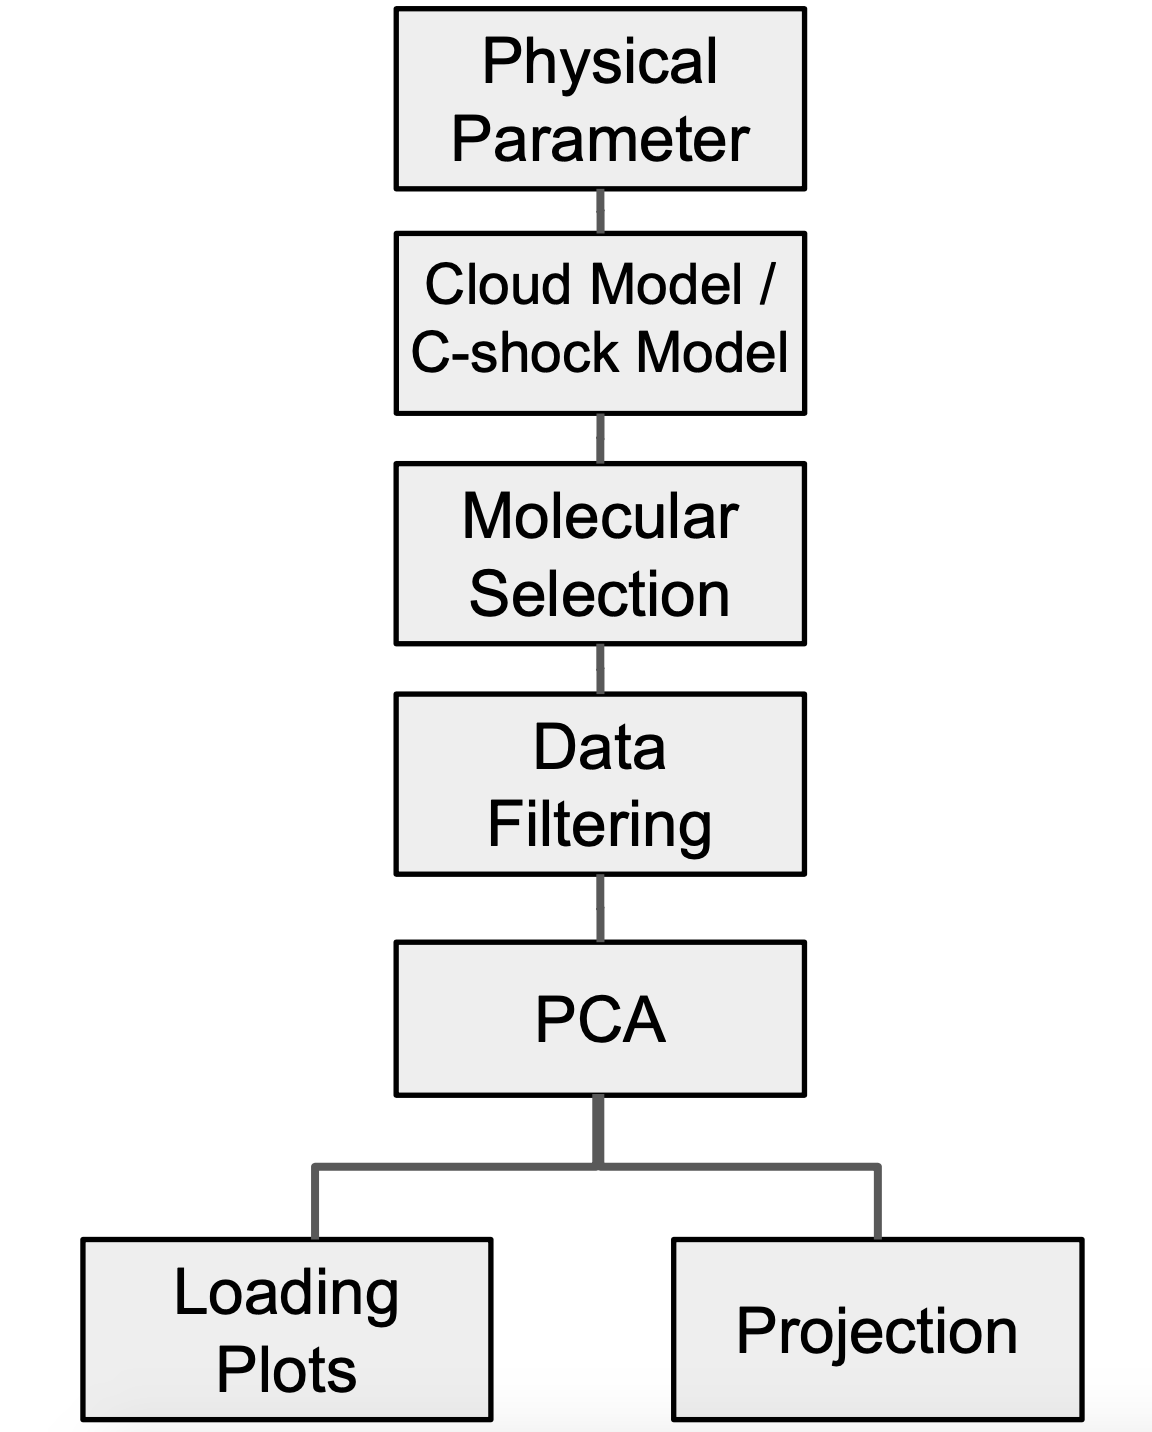
\includegraphics[angle=0,scale = 0.3]{flowchart-3.png}
   \caption{Flowchart of analysis process.}
         \label{Fig1}
   \end{figure}

%-------------------RESULTS------------------------
\section{Results}

\subsection{UCLCHEM models}

  Based on the simulation outputs of cloud models, three groups of relatively simple and commonly observed molecules were  selected for data analysis. The selection was also guided by the completeness of the chemical network. The corresponding results are interpreted in the following subsections. Table~\ref{tab:molegroups} summarises the groups of species analysed.
 

  \begin{table*}[htbp]
\centering
\begin{tabular}{ccccccccc}
\hline\hline
Group & \multicolumn{8}{c}{Molecular Species}                         \\ \hline
C1    & \multicolumn{8}{c}{CO, HCO$^+$, CS, SiO, HCN, NH$_3$, HNC}          \\
C2    & \multicolumn{8}{c}{CO, HCO$^+$, CS, SiO, HCN, HNC}         \\
C3    & \multicolumn{8}{c}{CO, HCO$^+$, CS, SiO, HCN}         \\
S1    & \multicolumn{8}{c}{SiO, HCO$^+$, CH$_3$OH, H$_2$CS, HNCO, NH$_3$, OCS, CO} \\
S2    & \multicolumn{8}{c}{CO, HCO$^+$, CS, SiO, HCN, NH$_3$, HNC}         \\
S3    & \multicolumn{8}{c}{CO, HCO$^+$, CS, SiO, HCN, HNC, HNCO, CH$_3$OH, N$_2$H$^+$}      \\
\hline\hline
\end{tabular}
\caption{Groups of molecules explored in the PCA analysis. C1, C2, and C3 are chemical models. S1, S2, and S3 are C-shock models.}
\label{tab:molegroups}
\end{table*}

  
  
\subsubsection{Group C1 (CO, HCO$^+$, CS, SiO, HCN, NH$_3$, and HNC)}
   
  The results of simulation generate more than two hundred molecules, in the Gourp C1, only seven of them: 
  CO, HCO$^+$, CS, SiO, HCN, NH$_3$ and HNC, are selected. 
  There are three considerations when selecting the group of molecues.  
  Firstly, those molecules are based on producing a large suite of models analysed here, a reduced chemical network was used which focused on the evolution of simple species \citep{holdship2017uclchem}. 
  Secondly, these molecules are commonly observed in observations. 
  Thirdly, considering the molecular fractions, those seven molecules are the most abundant of the simple molecular species. 
  After the selection progress has been done, the data can be viewed as a $200000\times7$ matrix. 
  Besides, we also take the numerical uncertainty into consideration. 
  Before making any analysis, we filter the abundances to only include values greater than $1.0\times10^{-13}$. 
  Below this value, the abundances are unreliable due to numerical noise. 
  After the filtering progress has been done, the data can be viewed as a $150283\times7$ matrix.  
  
  In this section, we describe the results of the PCA analysis of Group C1, consisting of seven frequently observed and common species: CO, HCO$^+$, CS, SiO, HCN, NH$_3$, and HNC. 
  Fig. \ref{Fig-cloud-7-variance} and Table \ref{table-7-eigenvalue} shows the individual and cumulative explained variance of the seven principal components (PCs). The first three PCs are the most significant components, representing $85.3\%$ of the total variance, the individual explained variance ratios of them is PC1: $50.3\%$, PC2: $19.9\%$ and PC3: $15.0\%$.
  
  %%%%%%------------   Figure ------------------------ 
  \begin{figure}[htbp]
   \centering
   \captionsetup{justification=centering}
   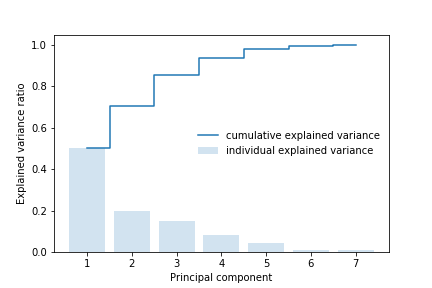
\includegraphics[angle=0,scale = 0.6]{7/explained_variance_ratio.png}
   \caption{Individual and cumulative explained variance of PCs among Group C1 (CO, HCO$^+$, CS, SiO, HCN, NH$_3$, and HNC)}
         \label{Fig-cloud-7-variance}
   \end{figure}
   
%%--------------    Table 1 ----------------------


\begin{table*}[htbp]
\centering
\begin{tabular}{ccc}
\hline\hline
\multicolumn{1}{l}{Pincipal Components} & \multicolumn{1}{l}{Explained Ratio} & Cumulative Variance \\ \hline
PC1                                     & 0.503                               & 0.503               \\
PC2                                     & 0.199                               & 0.702               \\
PC3                                     & 0.150                               & 0.852               \\
PC4                                     & 0.083                               & 0.936               \\
PC5                                     & 0.045                               & 0.980               \\
PC6                                     & 0.012                               & 0.992               \\
PC7                                     & 0.008                               & 1.000   \\           \hline\hline
\end{tabular}
\caption{Table of individual and cumulative explained variance of PCs among seven molecules in Group C1 (CO, HCO$^+$, CS, SiO, HCN, NH$_3$, and HNC).}
\label{table-cloud-1}
\end{table*}
   
   PCs and their eigenvalues quantify the significance of gradients in the data. 
   As listed in Table~\ref{table-7-eigenvalue}, in the direction of PC1, the eigenvalues of seven molecules are all negative, the most influential four of them are CO(-0.511), HNC(-0.495), HCN(-0.466), and NH$_3$(-0.457).
   Since they all have negative sign, their projection on PC1 is in the opposite direction as PC1.
%   The negative sign indicates the eigenvector has opposite direction compared with the PC. 
   Table \ref{table-7-eigenvalue} also shows that PC2 contains quite high loading value of HCO$^+$ (0.728) and CS (-0.598). 
   Although containing a lower proportion of the overall structure, PC3 is typically dominated by SiO, with a contribution of 0.944.
   While the loading value for other molecules is not larger than 0.241, which is from NH$_3$, the direction of its projection is opposite to SiO in this PC.
   %This situation represents that the SiO has overwhelming contribution on PC3. 



%%%%% -----------table------------
\begin{table*}[htbp]
\centering
\begin{tabular}{cccccccc}
\hline\hline
\multirow{2}{*}{Molecular Species} & \multicolumn{7}{c}{Principal Components}                 \\ \cline{2-8} 
                                   & 1       & 2       & 3       & 4       & 5      & 6    & 7\\ \hline
CO                                  & -0.511 & -0.100 & 0.072  & -0.142 & -0.096 & 0.487  & 0.675  \\ \hline
HCO$^+$                               & -0.001 & 0.728  & 0.118  & -0.620 & 0.264  & -0.006 & 0.007  \\ \hline
CS                                 & -0.249 & -0.598 & 0.138  & -0.659 & 0.038   & -0.253 & -0.243 \\ \hline
SiO                                & -0.059 & -0.001 & 0.944   & 0.259  & 0.187  & -0.028 & -0.044 \\ \hline
HCN                                & -0.466 & 0.257  & 0.060    & 0.044  & -0.610 & 0.202   & -0.545 \\ \hline
NH3                                & -0.457 & -0.024 & -0.241 & 0.223  & 0.714  & 0.231  & -0.343 \\ \hline
HNC                                & -0.495 & 0.185  & -0.092 & 0.200  & -0.027 & -0.776 & 0.260 \\ \hline\hline
\end{tabular}
\caption{Eigenvalues of the PCA for the seven molecules in Group C1 (CO, HCO$^+$, CS, SiO, HCN, NH$_3$, and HNC).}
\label{table-7-eigenvalue}
\end{table*}
   
   The loading plots in Fig. \ref{Fig-7-loading} provide an intuitive way to illustrate the eigenvalues of PCs. 
   Since the top three PCs are the most significant, they are selected to generate loading plots. 
   Fig. \ref{Fig-7-loading-12} shows that on PC1, four molecules (CO, HNC, HCN, and NH$_3$) contribute mainly on this PC, which on PC2, HCO$^+$ and CS are the most influential features.
   %, same as the conclusion we obtained from Table \ref{table-7-eigenvalue}. 
   However, the contribution of SiO is non-negligible in PC3. 
   Loading plots also reveal the correlation between different features \citep{al2015principal}.
   In Fig. \ref{Fig-7-loading-12}, the acute angle between HCN and HNC indicates that they are highly and positively correlated, same as CO and NH$_3$. 
   HCO$^+$ and NH$_3$ are almost perpendicular with each other, which demonstrates that on this plane they are not likely to be correlated. Fig. \ref{Fig-7-loading-23} shows that the SiO is the most influential molecule on PC3 while the other species contribute at much lower levels. 
   In Fig. \ref{Fig-7-loading-23}, it is remarkable that the obtuse angle between CS and HCO$^+$ shows they are negatively correlated.
   
   
      %%%------------Figure 3-----
\begin{figure}[htbp]
\centering  
\subfigure[Plane of PC1 and PC2]{
\label{Fig-7-loading-12}
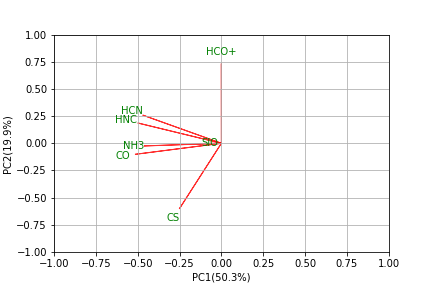
\includegraphics[width=0.5\textwidth]{7/loadingplot_PC1&2.png}}
\subfigure[Plane of PC2 and PC3]{
\label{Fig-7-loading-23}
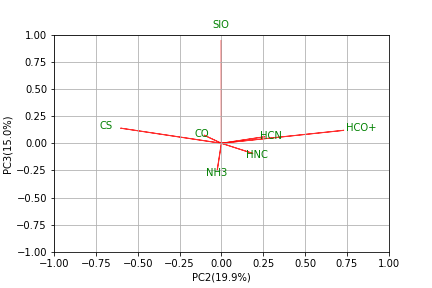
\includegraphics[width=0.5\textwidth]{7/loadingplot_PC2&3.png}}
\caption{Loading plots for the seven molecules in Group C1 (CO, HCO$^+$, CS, SiO, HCN, NH$_3$, and HNC).}
\label{Fig-7-loading}
\end{figure}

   
    Fig. \ref{C1-12}, Fig. \ref{C1-23}, and Fig. \ref{C1-34} show the projection of a full sample of UCLCHEM models onto planes of the principal component vectors derived from the Group C1 species. 
    In the figures of projection, the points represent that each model is colour-coded by a physical parameter. 
    This allows us to investigate the relationship between the components and particular physical parameters. 
    If they are, then plotting observations of the group of molecules in these planes would allow the direct inference of the physical conditions in the gas. 
    
    Introducing the physical parameters can reveal any trend hidden behind values that are not obvious in the original data sets. 
    However, only the limited physical parameters demonstrate observable tendency. 
    Fig. \ref{C1-12-maxtemp} indicates that the physical parameter maximum temperature has an increasing trend along the PC2, which is also can be viewed in Fig. \ref{C1-23-maxtemp}. 
    Fig. \ref{C1-12-metallicity} shows that the physical parameter metallicity has a decreasing trend along the PC1. 
    Moreover, Fig. \ref{C1-23-av} and Fig. \ref{C1-34-av} indicate that the physical parameter A\textsubscript{V} goes up in the direction of PC3.
    While the physical parameter initial density shows a decreasing trend along the direction of PC3, as shown in Fig. \ref{C1-23-initialdens} and Fig. \ref{C1-34-initialdens}. 
    Table \ref{table-7-all} shows these trends, where the negative sign demonstrates decreasing trend, and the positive sign indicates an increasing trend. 
    %%5-----------------------
 \begin{figure*}[htbp]
\centering
\subfigure{
\label{C1-12-av}
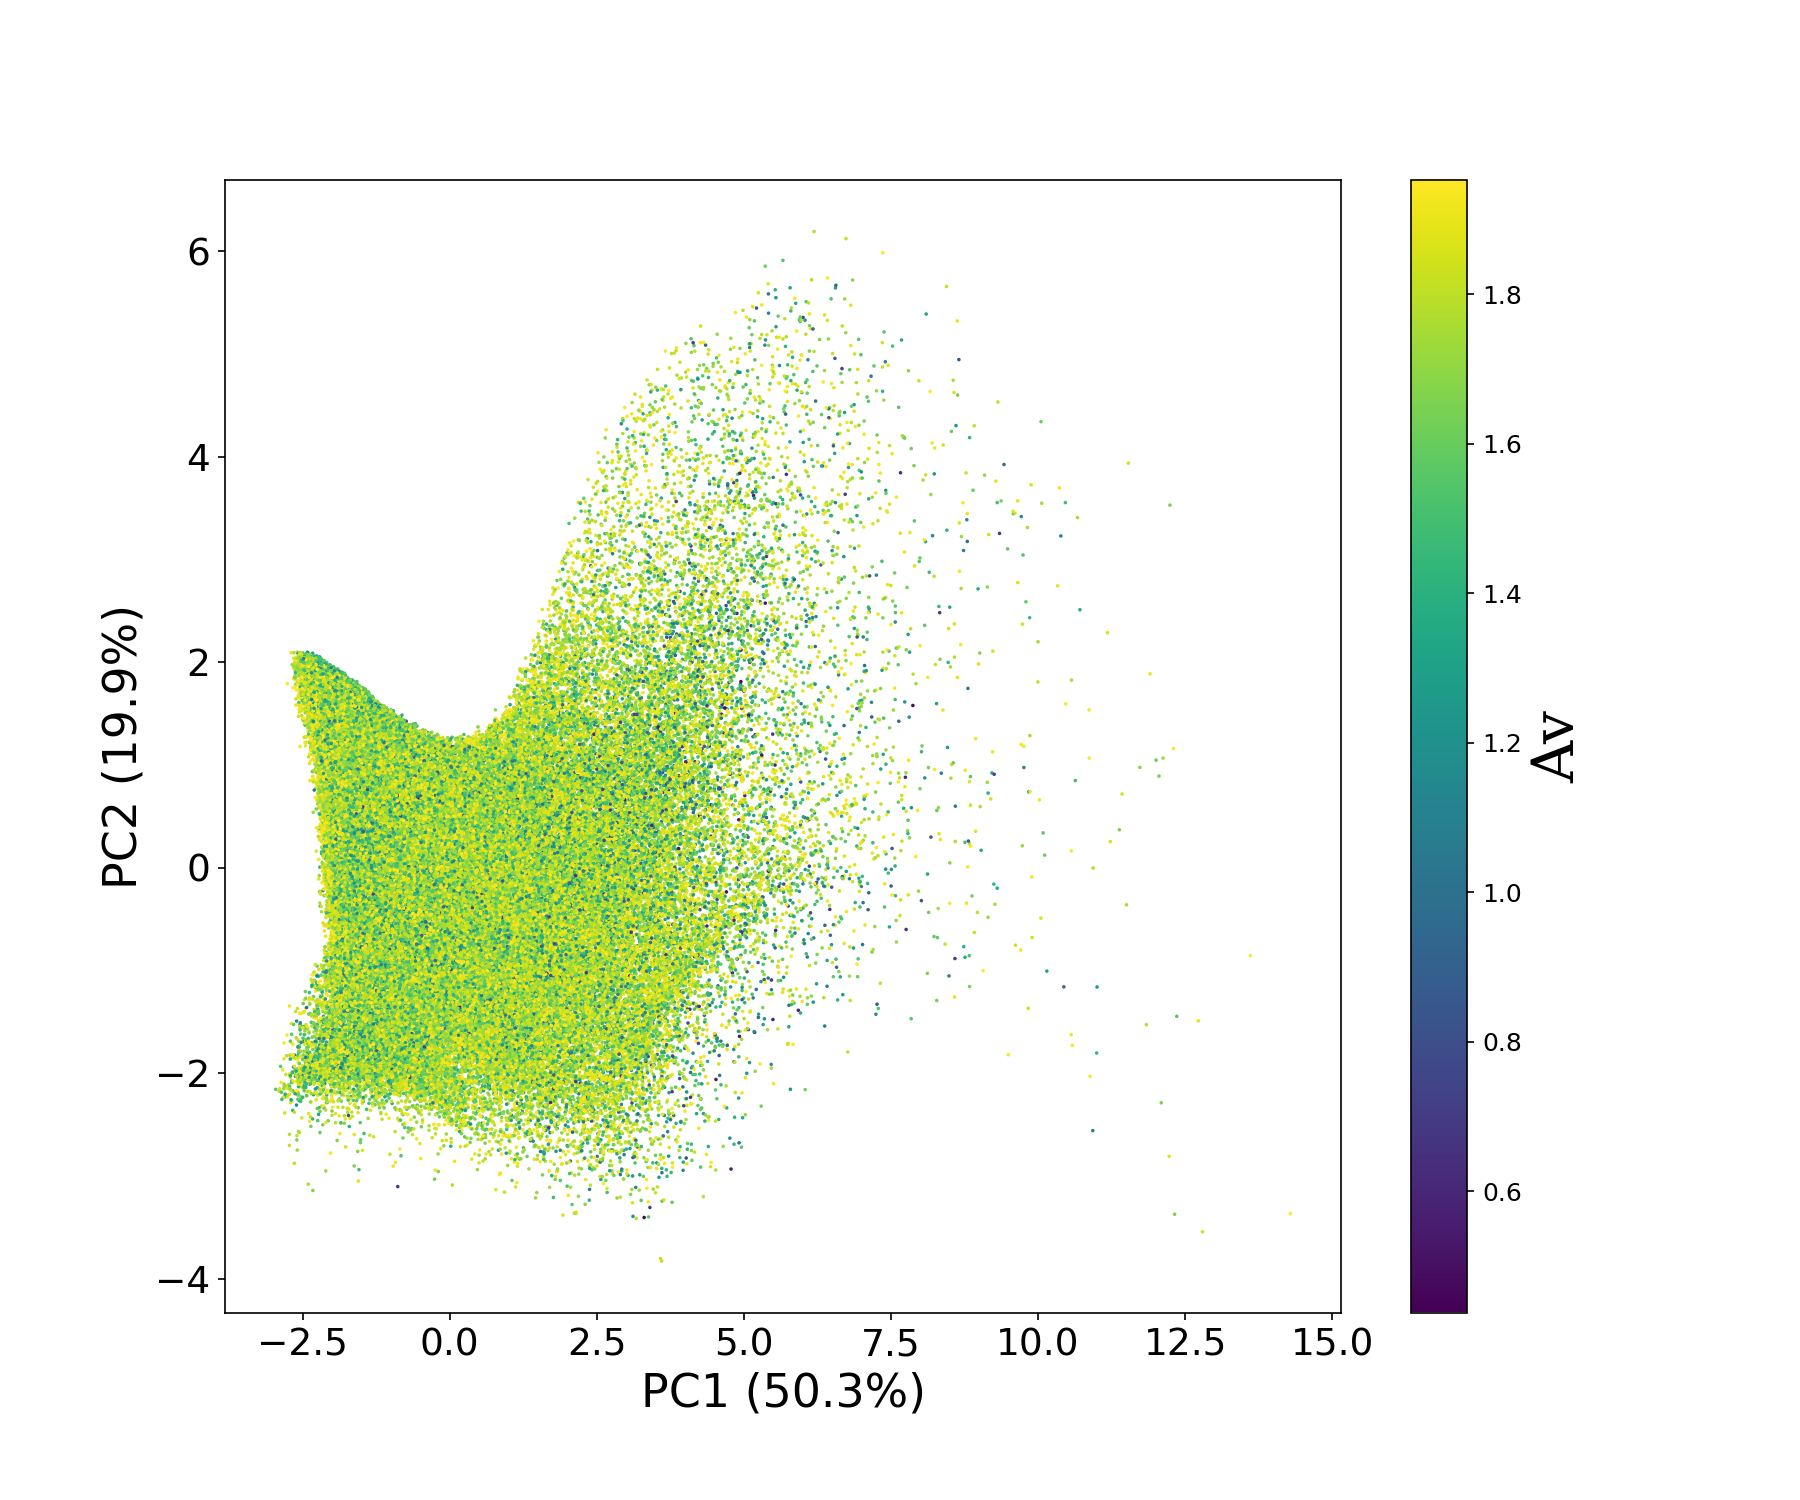
\includegraphics[width=5.9cm]{7/PC1&2_av.png}
}
\subfigure{
\label{C1-12-initialdens}
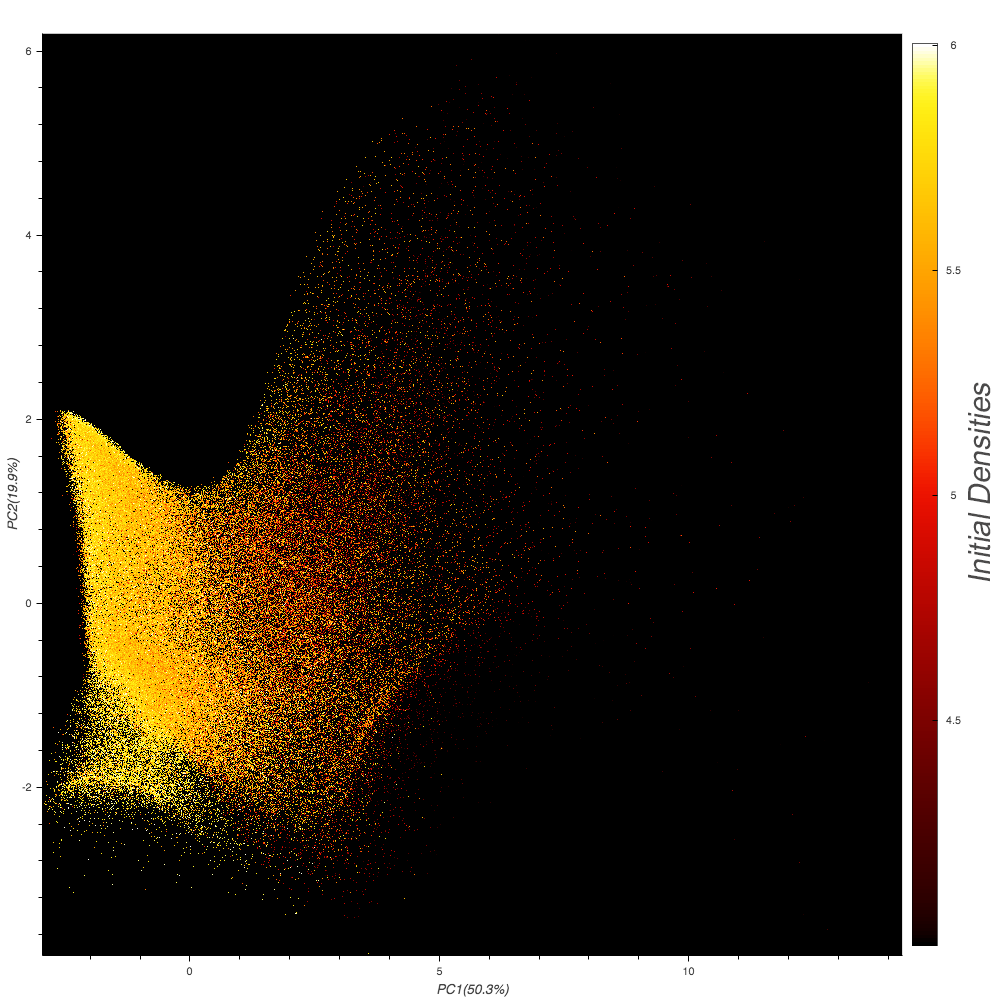
\includegraphics[width=5.9cm]{7/PC1&2_initialDens.png}
}
\subfigure{
\label{C1-12-maxtemp}
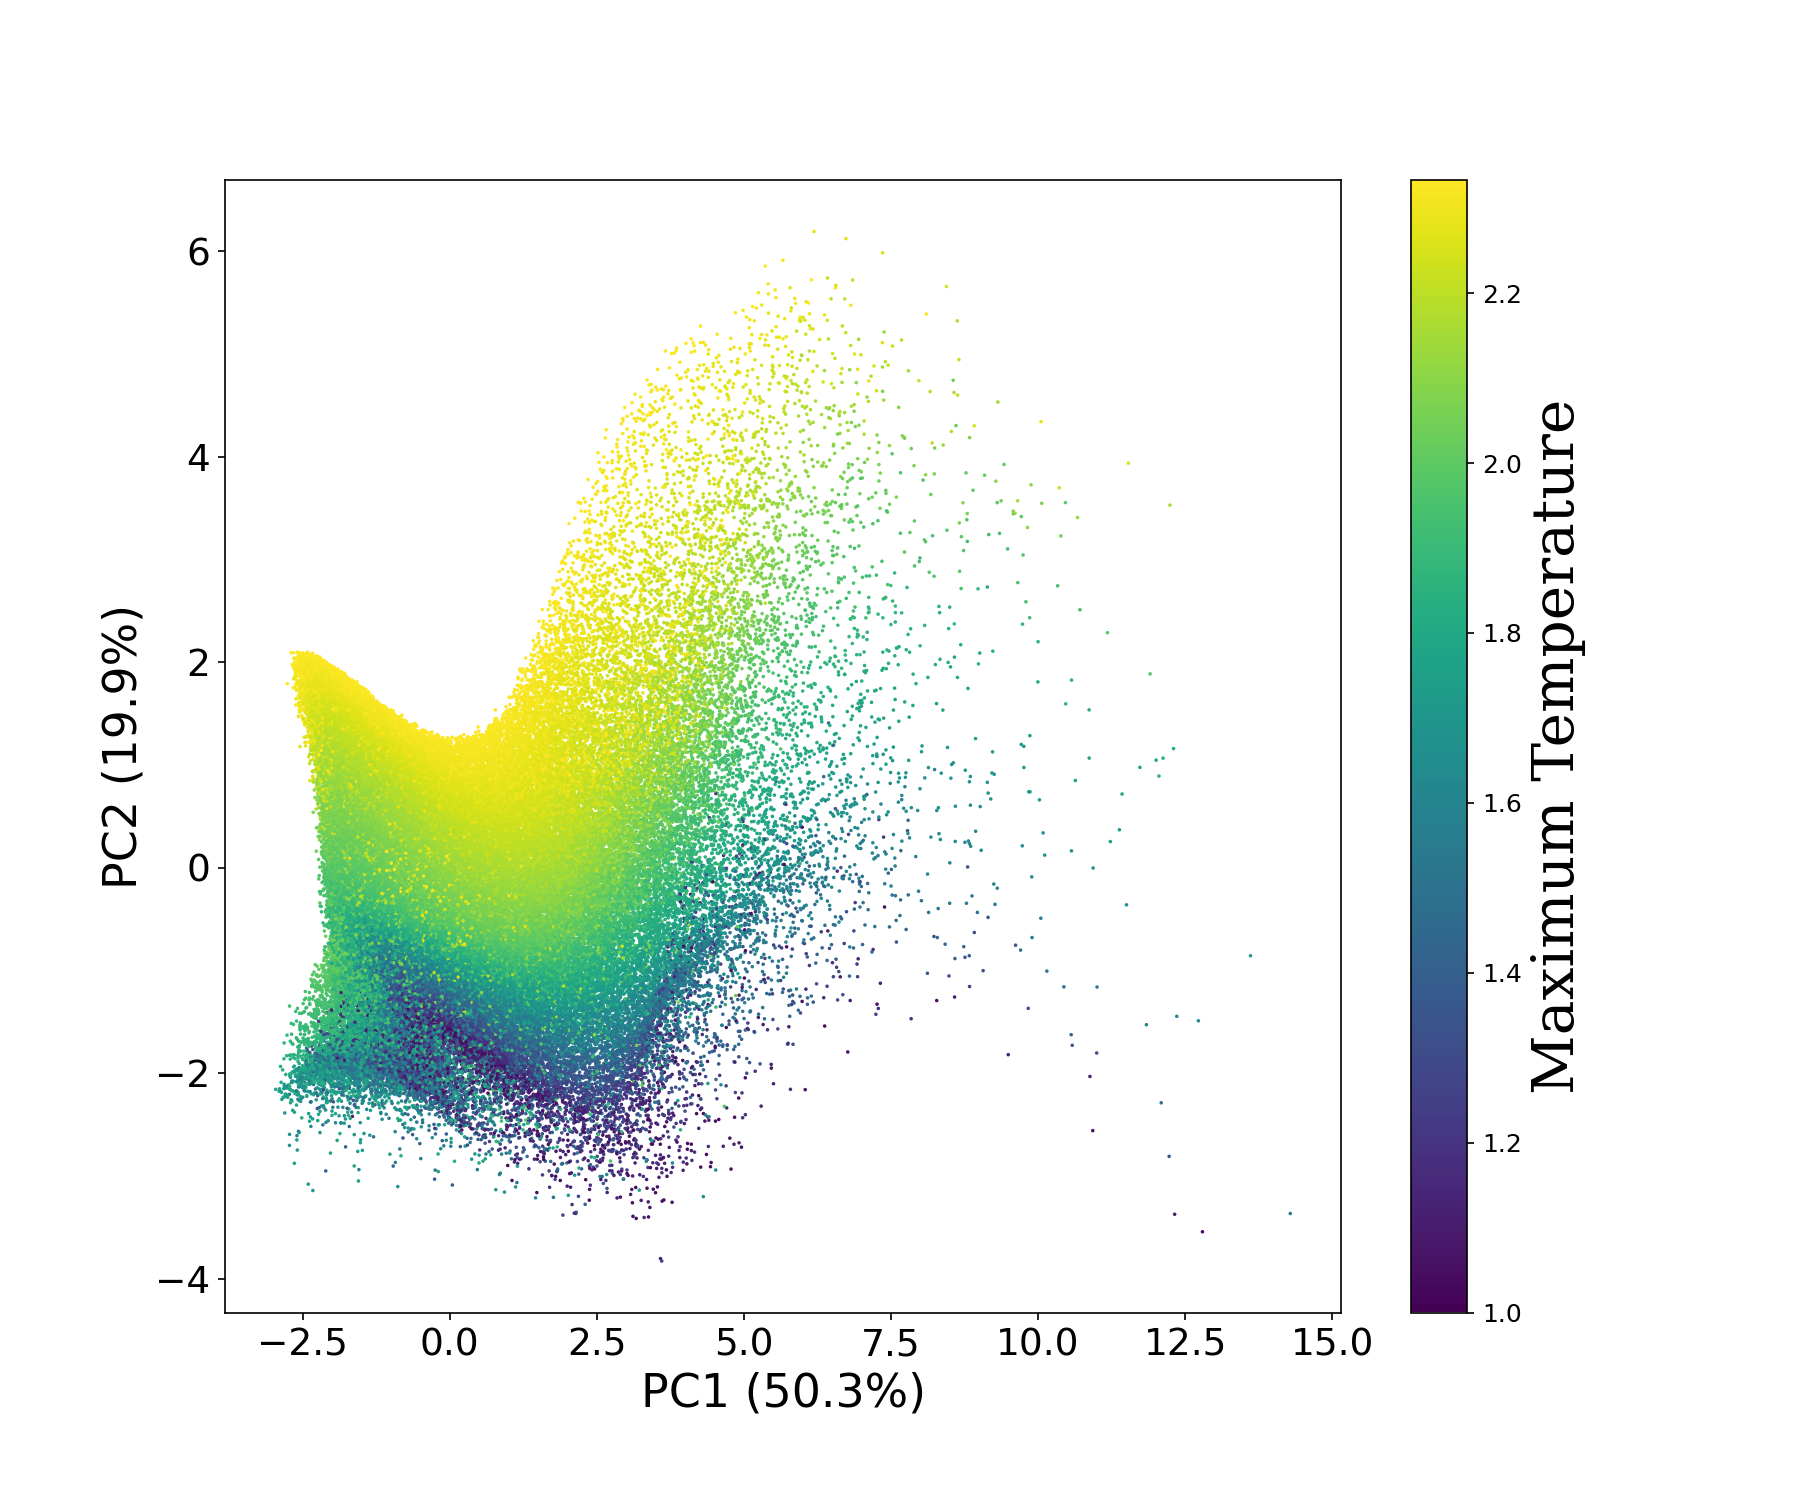
\includegraphics[width=5.9cm]{7/PC1&2_maxTemp.png}
} \\
\subfigure{
\label{C1-12-metallicity}
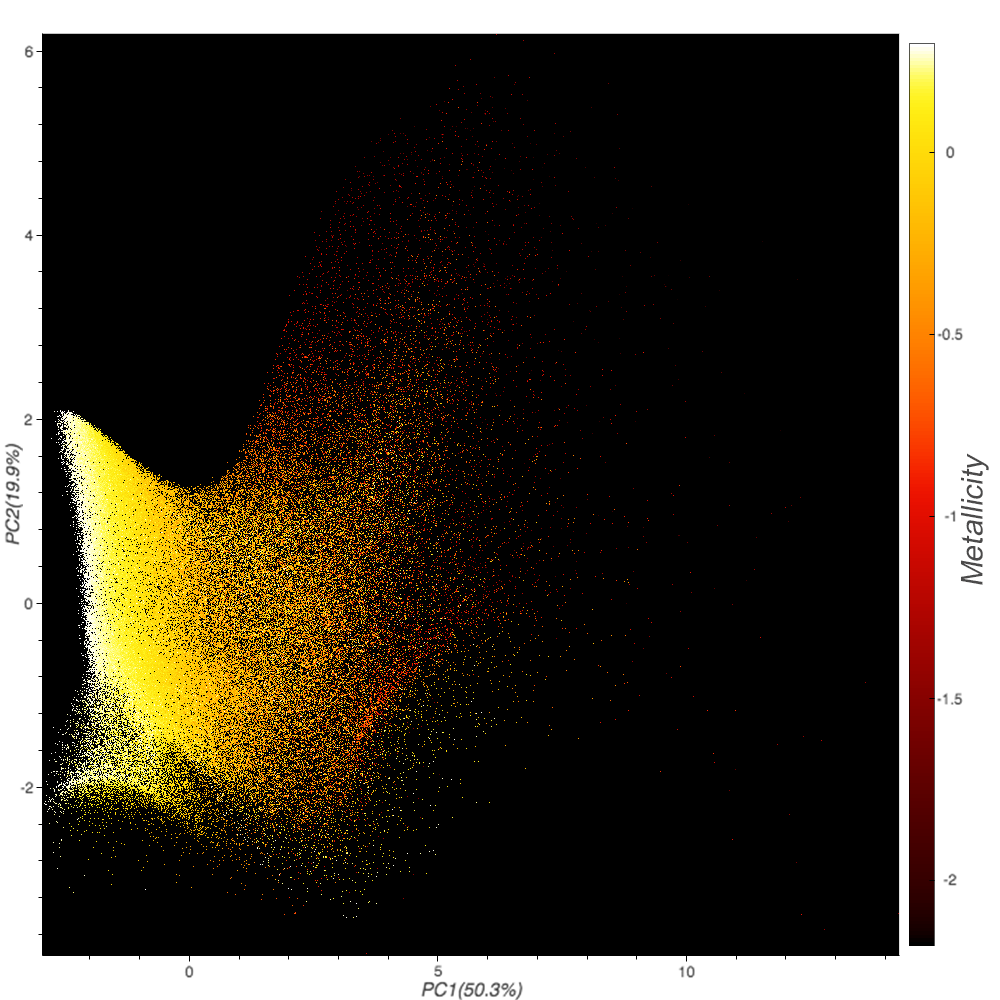
\includegraphics[width=5.9cm]{7/PC1&2_metallicity.png}
}
\subfigure{
\label{C1-12-radfield}
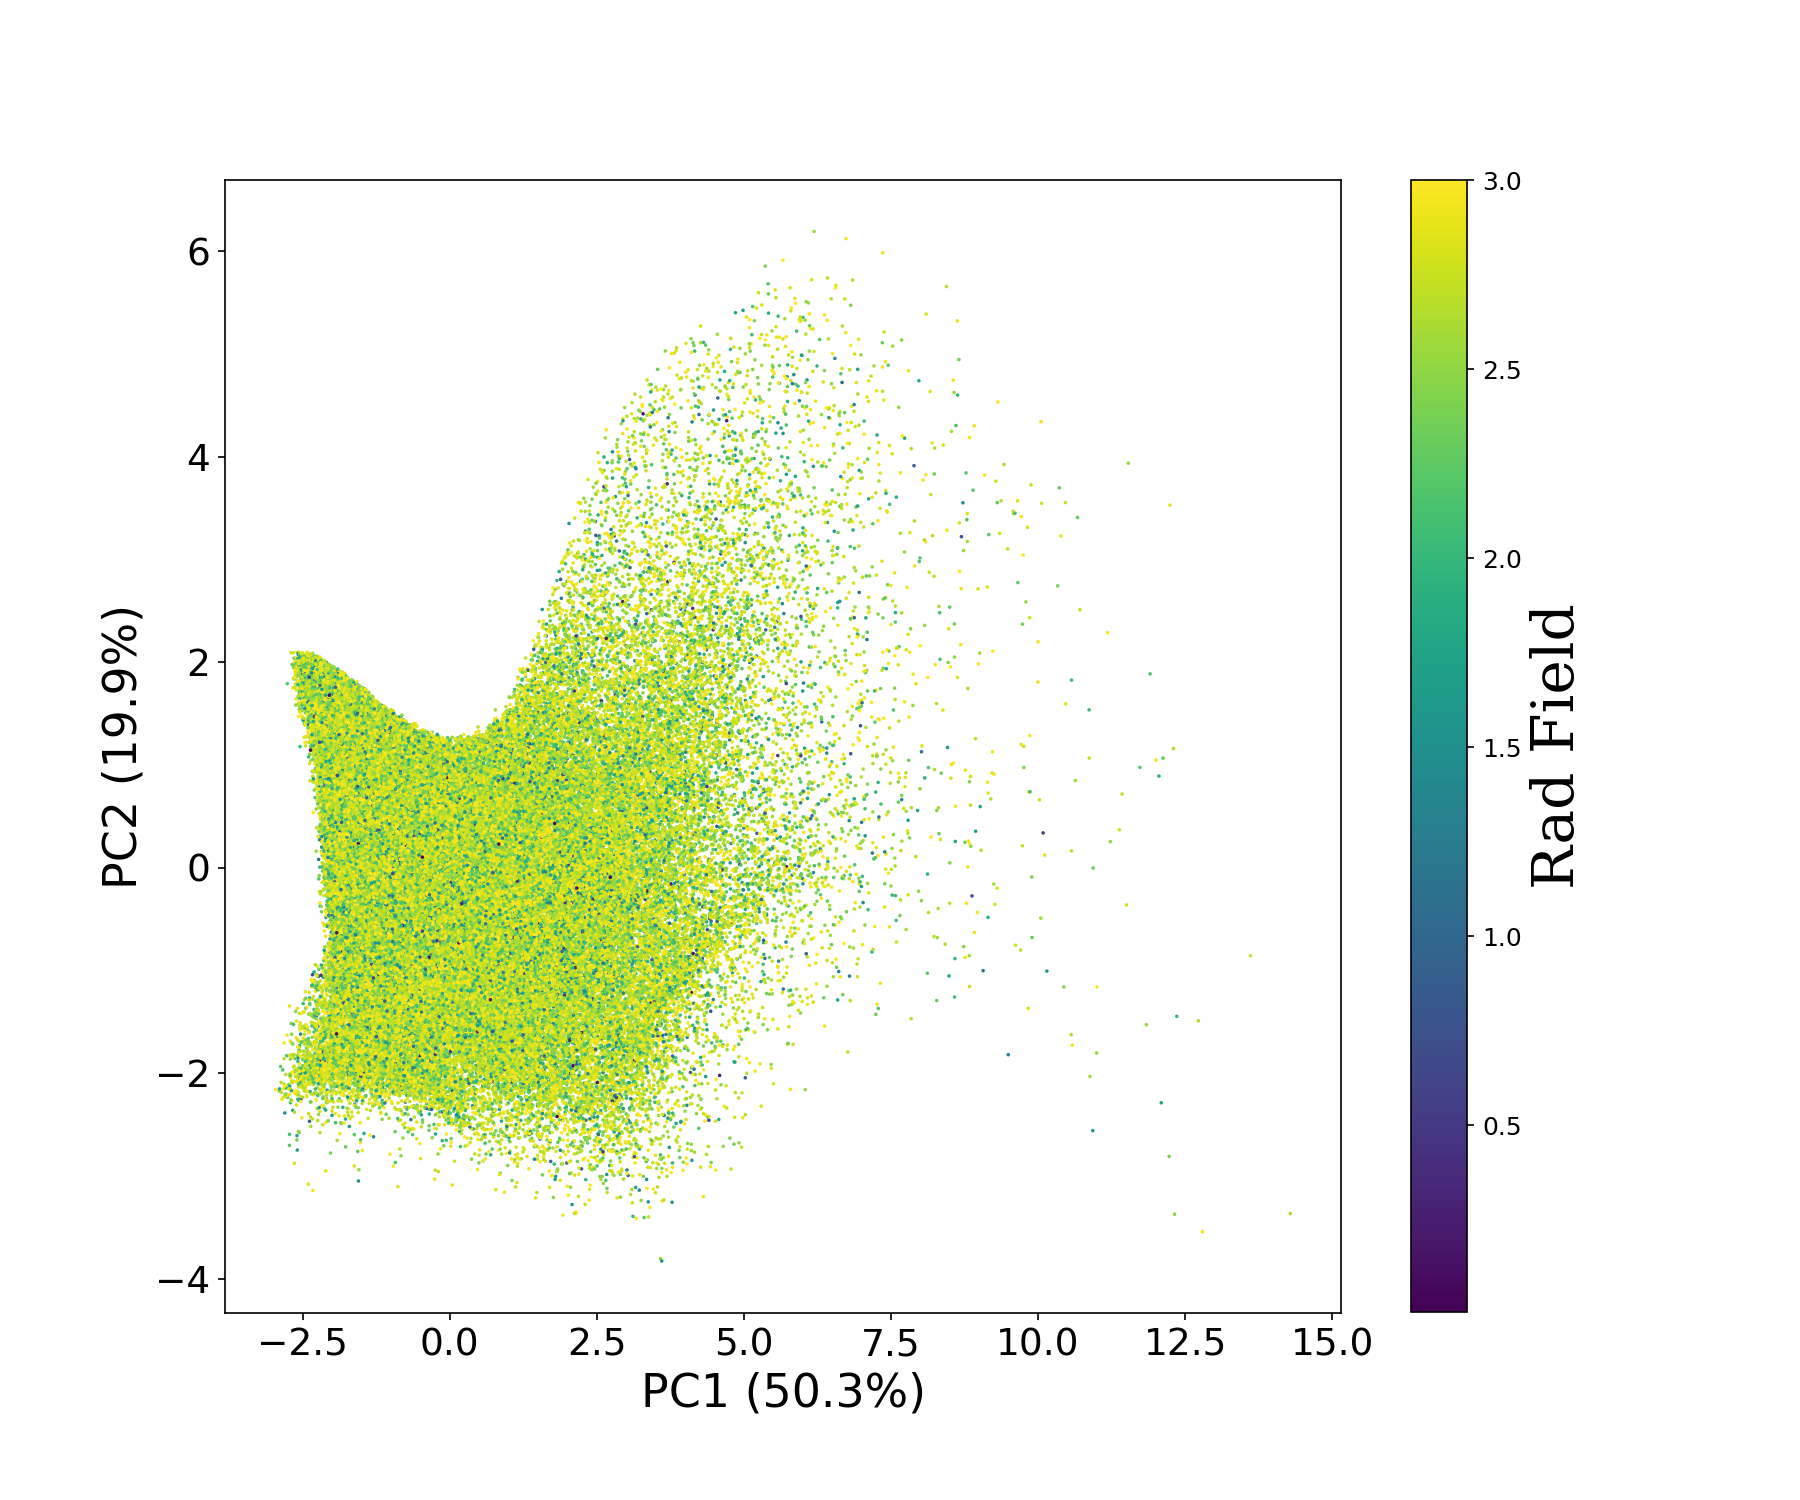
\includegraphics[width=5.9cm]{7/PC1&2_radfield.png}
}
\subfigure{
\label{C1-12-zeta}
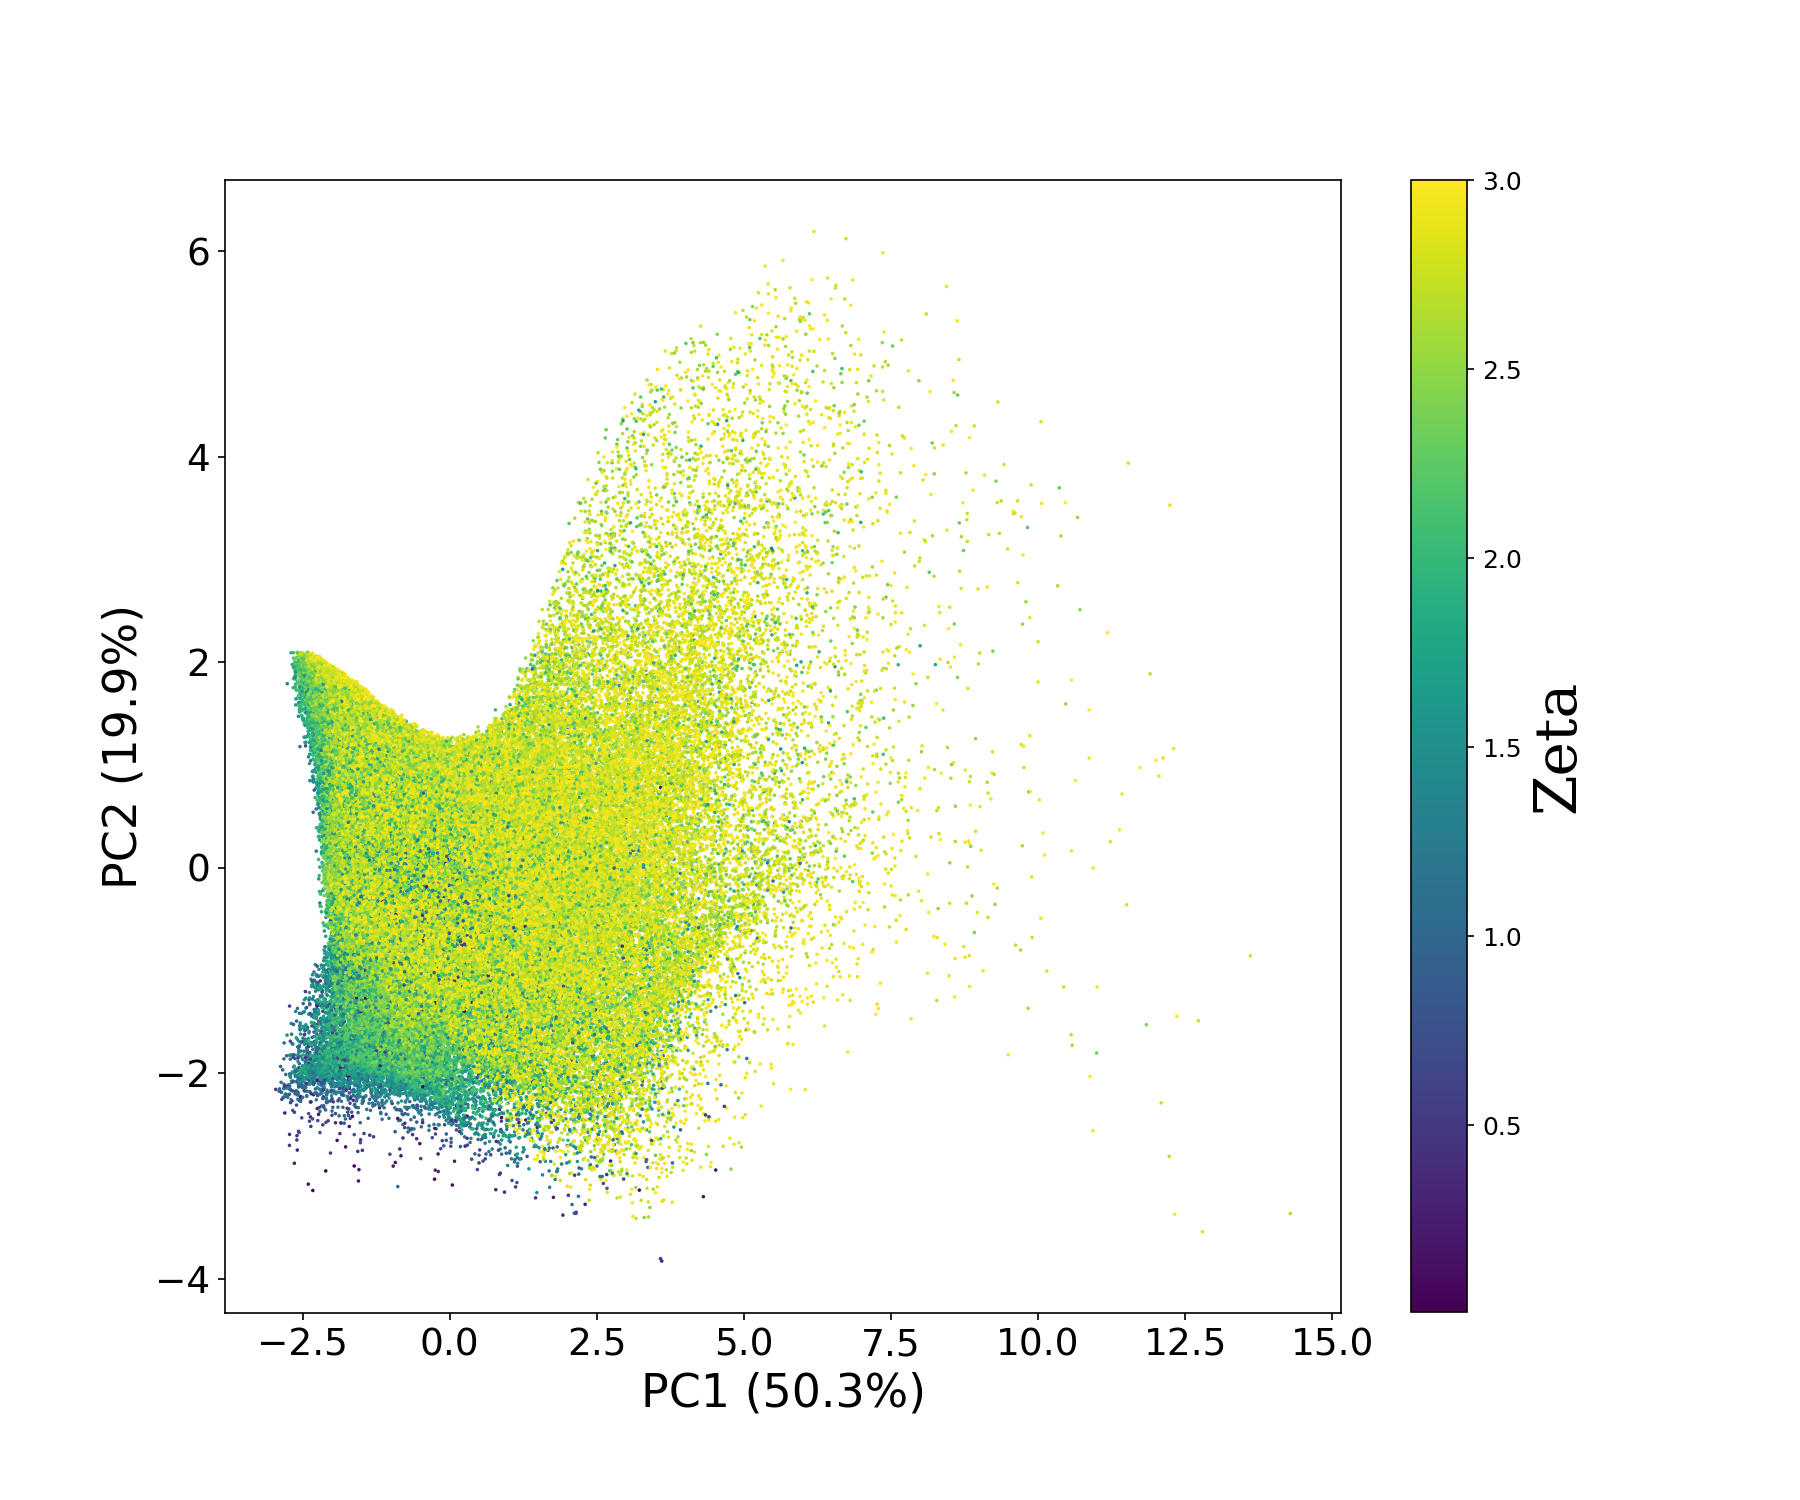
\includegraphics[width=5.9cm]{7/PC1&2_zeta.png}
}
\caption{Projection of Group C1 (CO, HCO$^+$, CS, SiO, HCN, NH$_3$, and HNC) on the plane of PC1 and PC2. Three panels on the top row are A\textsubscript{V}, initial densities and maximum temperature, while the three panels on the bottom row are metallicity, rad field and zeta, respectively. Among them, only the projection of maximum temperature and metallicity shows a clear trend.}
\label{C1-12}
 \end{figure*}
%%%%---------------
 \begin{figure*}[htbp]
\centering
\subfigure{
\label{C1-23-av}
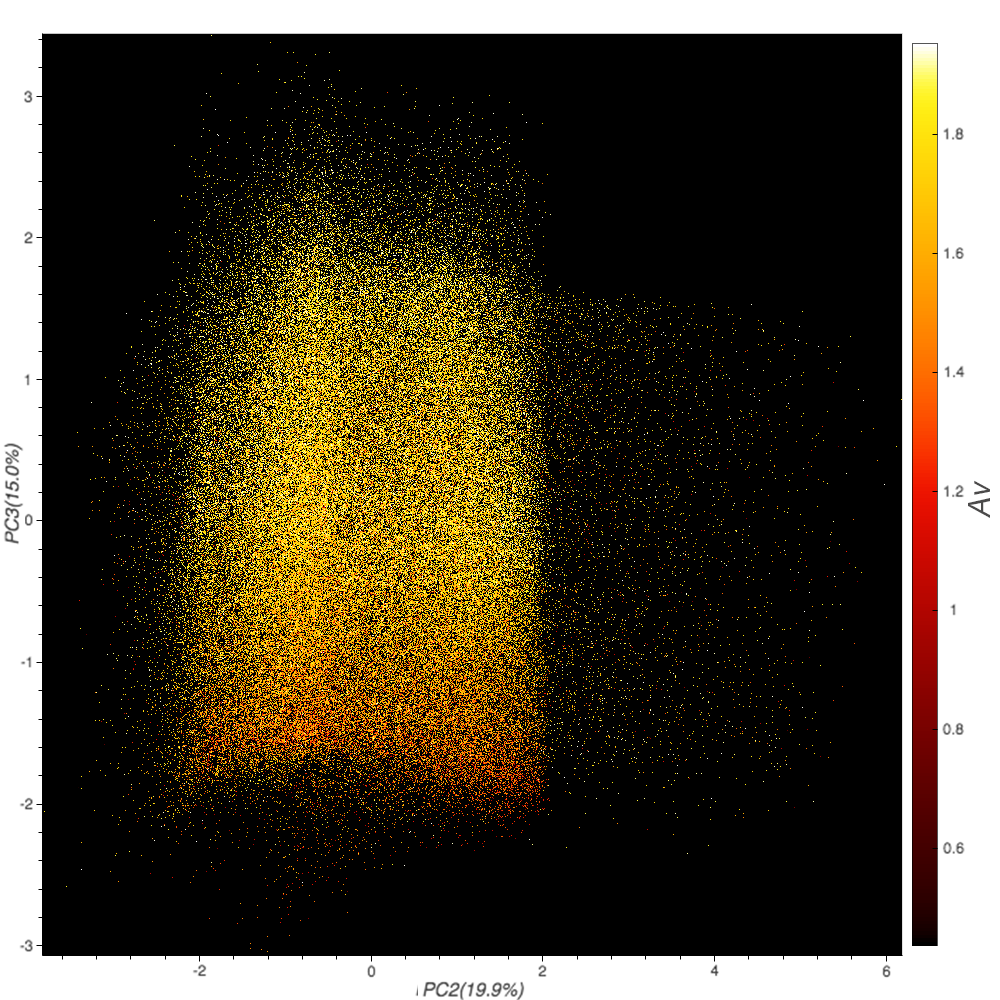
\includegraphics[width=5.9cm]{7/PC2&3_av.png}
}
\subfigure{
\label{C1-23-initialdens}
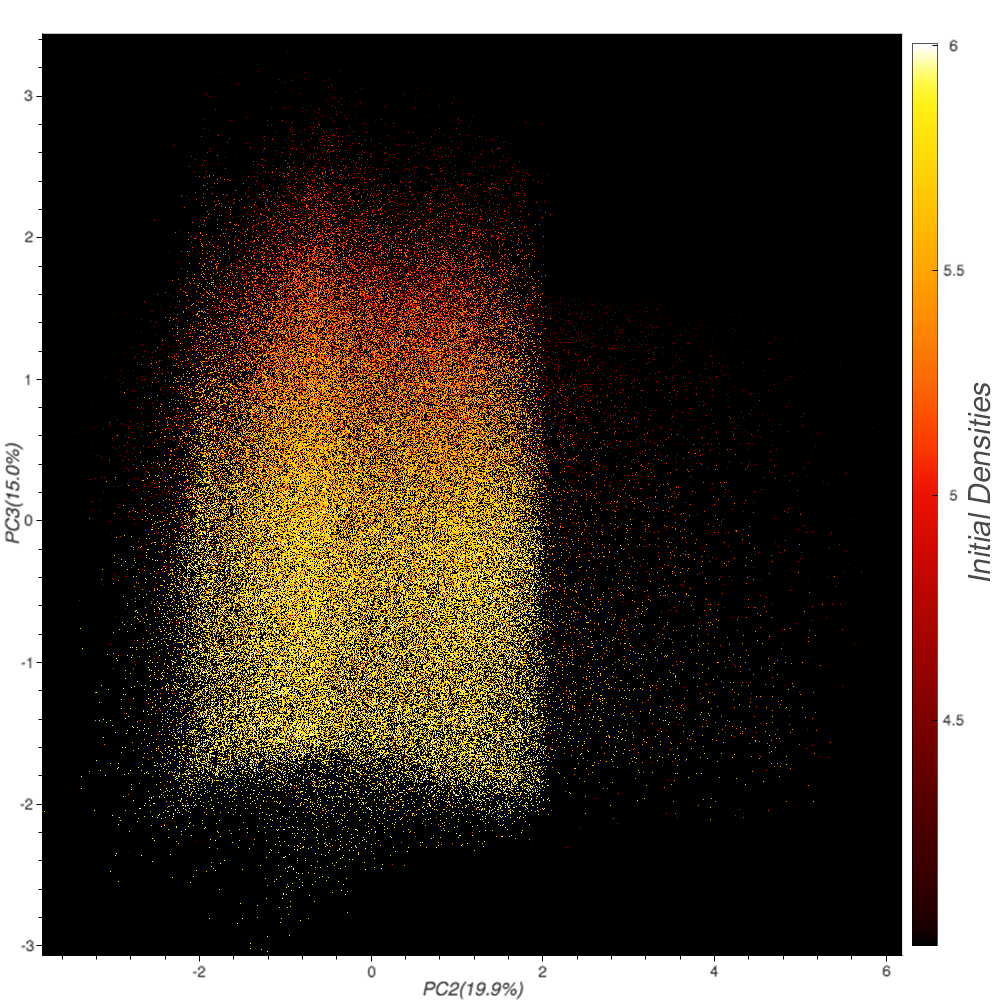
\includegraphics[width=5.9cm]{7/PC2&3_initialDens.png}
}
\subfigure{
\label{C1-23-maxtemp}
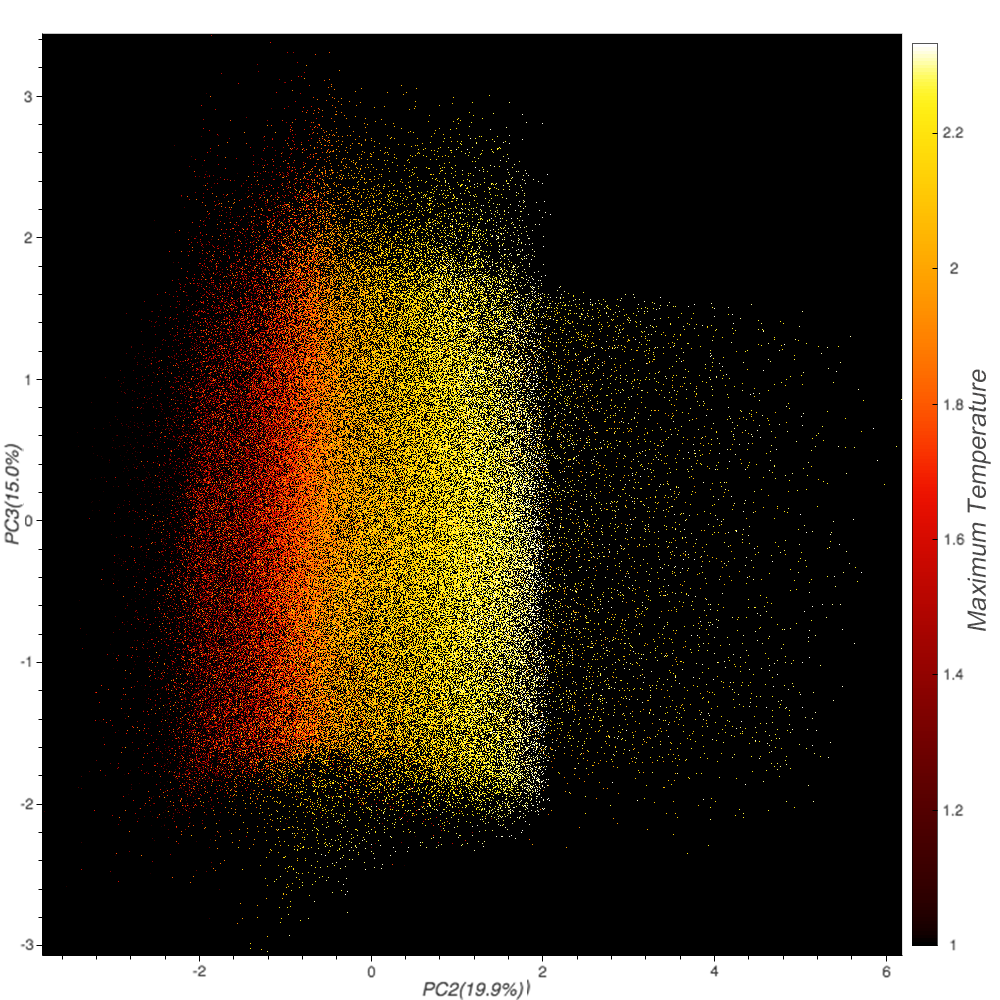
\includegraphics[width=5.9cm]{7/PC2&3_maxTemp.png}
}
\subfigure{
\label{C1-23-metallicity}
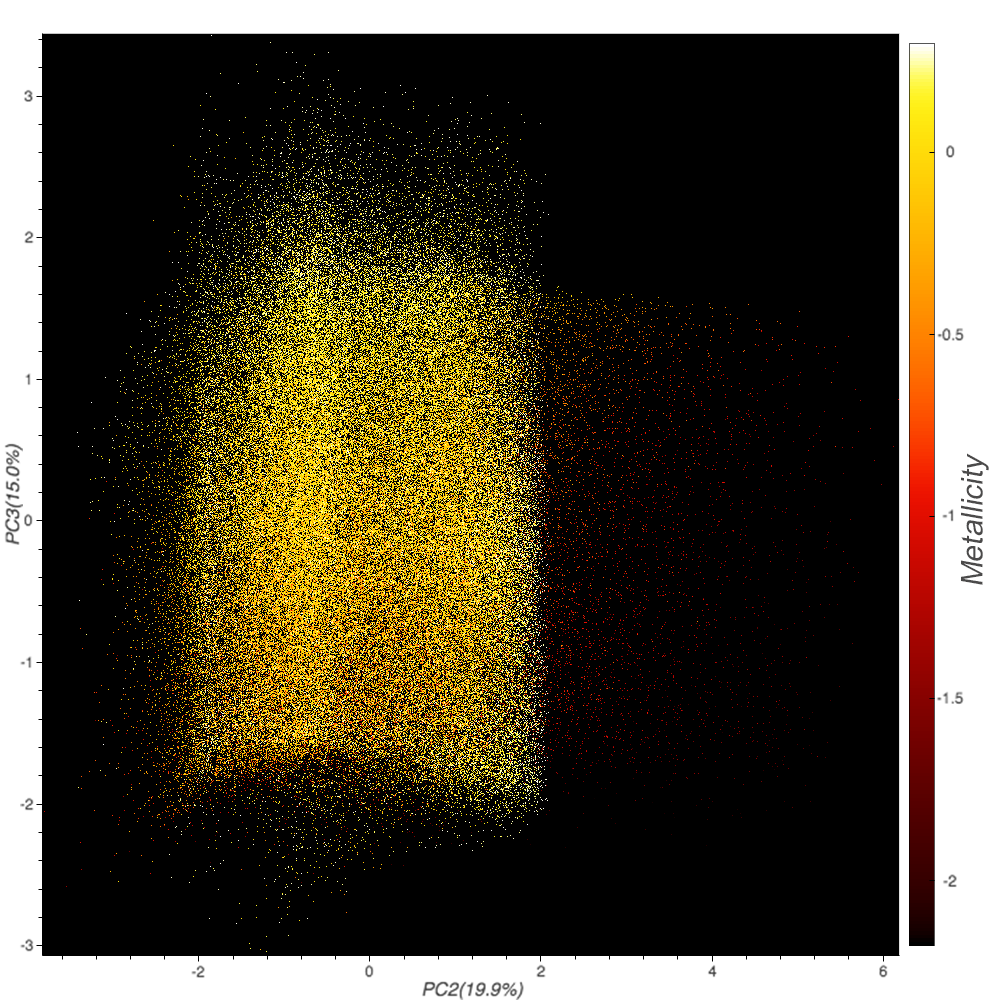
\includegraphics[width=5.9cm]{7/PC2&3_metallicity.png}
}
\subfigure{
\label{C1-23-radfield}
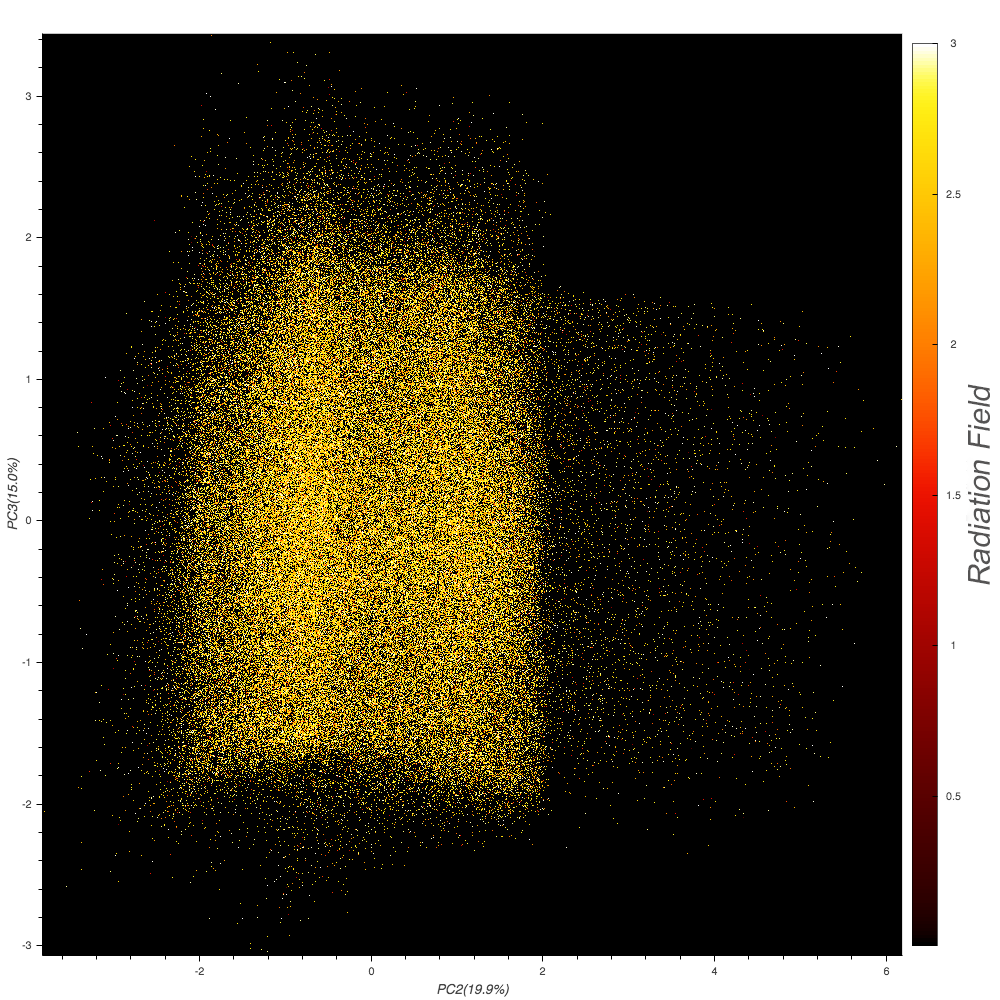
\includegraphics[width=5.9cm]{7/PC2&3_radfield.png}
}
\subfigure{
\label{C1-23-zeta}
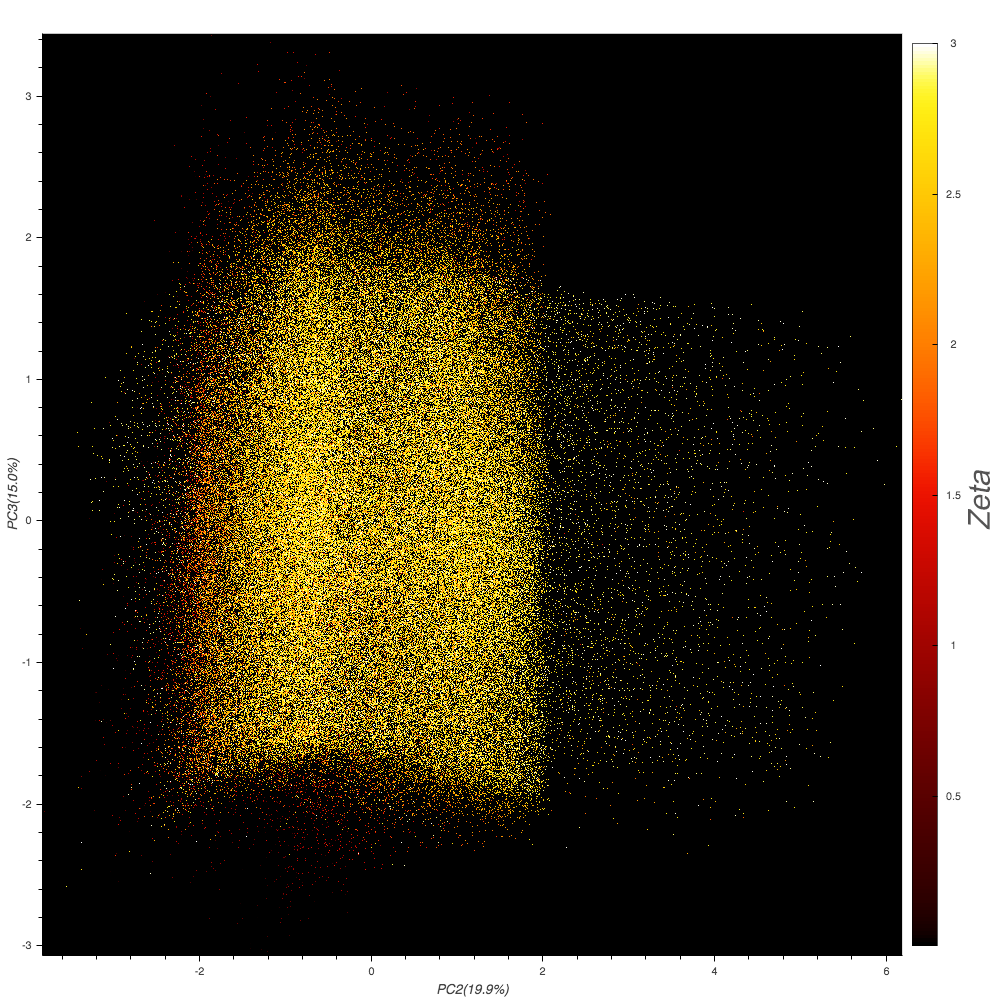
\includegraphics[width=5.9cm]{7/PC2&3_zeta.png}
}
\caption{Projection of Group C1 (CO, HCO$^+$, CS, SiO, HCN, NH$_3$, and HNC) on the plane of PC2 and PC3. Three panels on the top row are A\textsubscript{V}, initial densities and maximum temperature, while the three panels on the bottom row are metallicity, rad field and zeta, respectively. Among them, only the projection of maximum temperature and A\textsubscript{V} shows a clear trend.}
\label{C1-23}
 \end{figure*}
 
 %%%%----------------
\begin{figure*}[htbp]
\centering
\subfigure{
\label{C1-34-av}
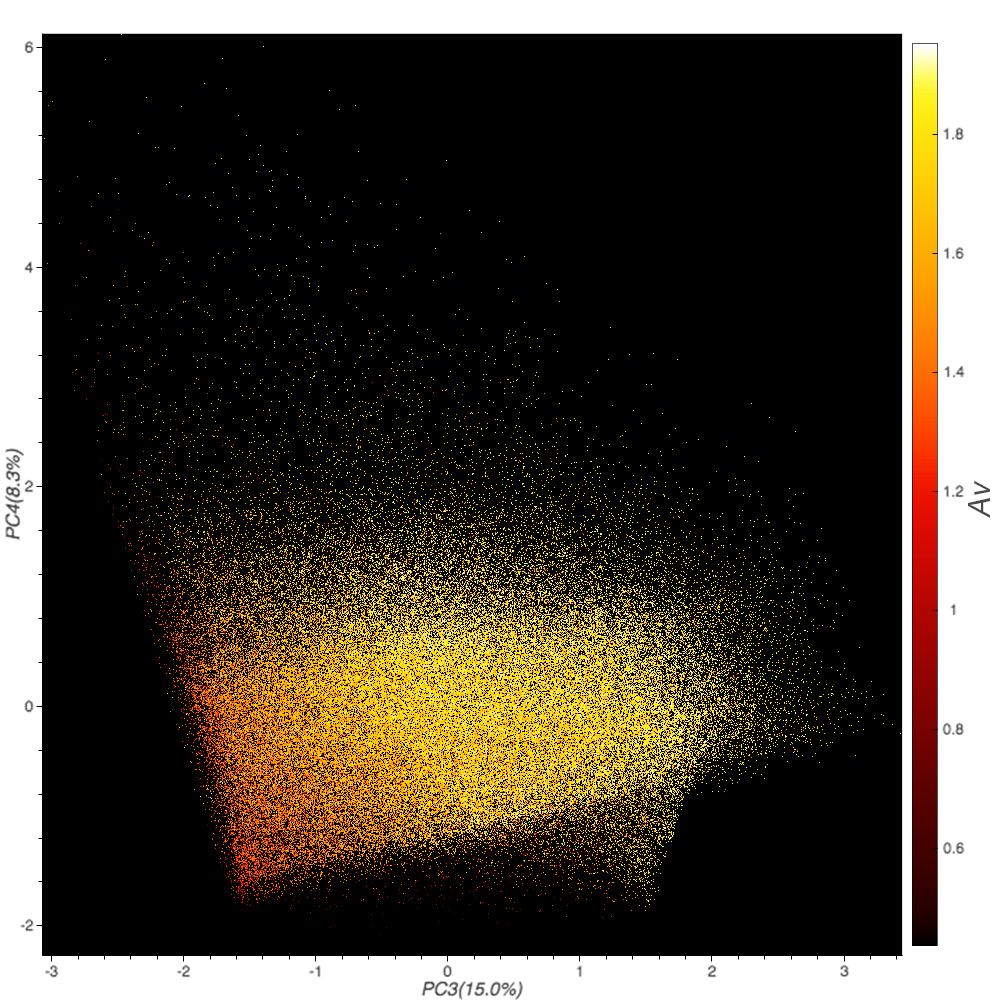
\includegraphics[width=5.9cm]{7/PC3&4_av.png}
}
\subfigure{
\label{C1-34-initialdens}
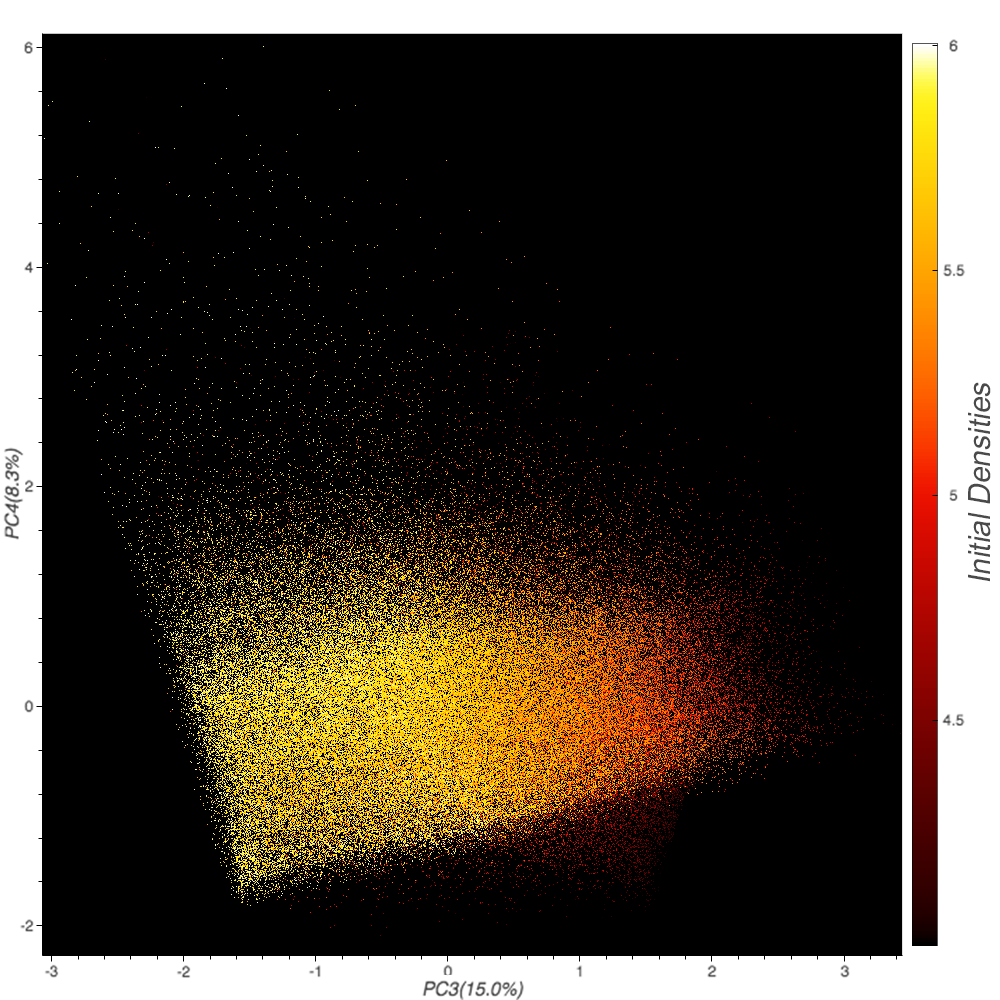
\includegraphics[width=5.9cm]{7/PC3&4_initialDens.png}
}
\subfigure{
\label{C1-34-maxtemp}
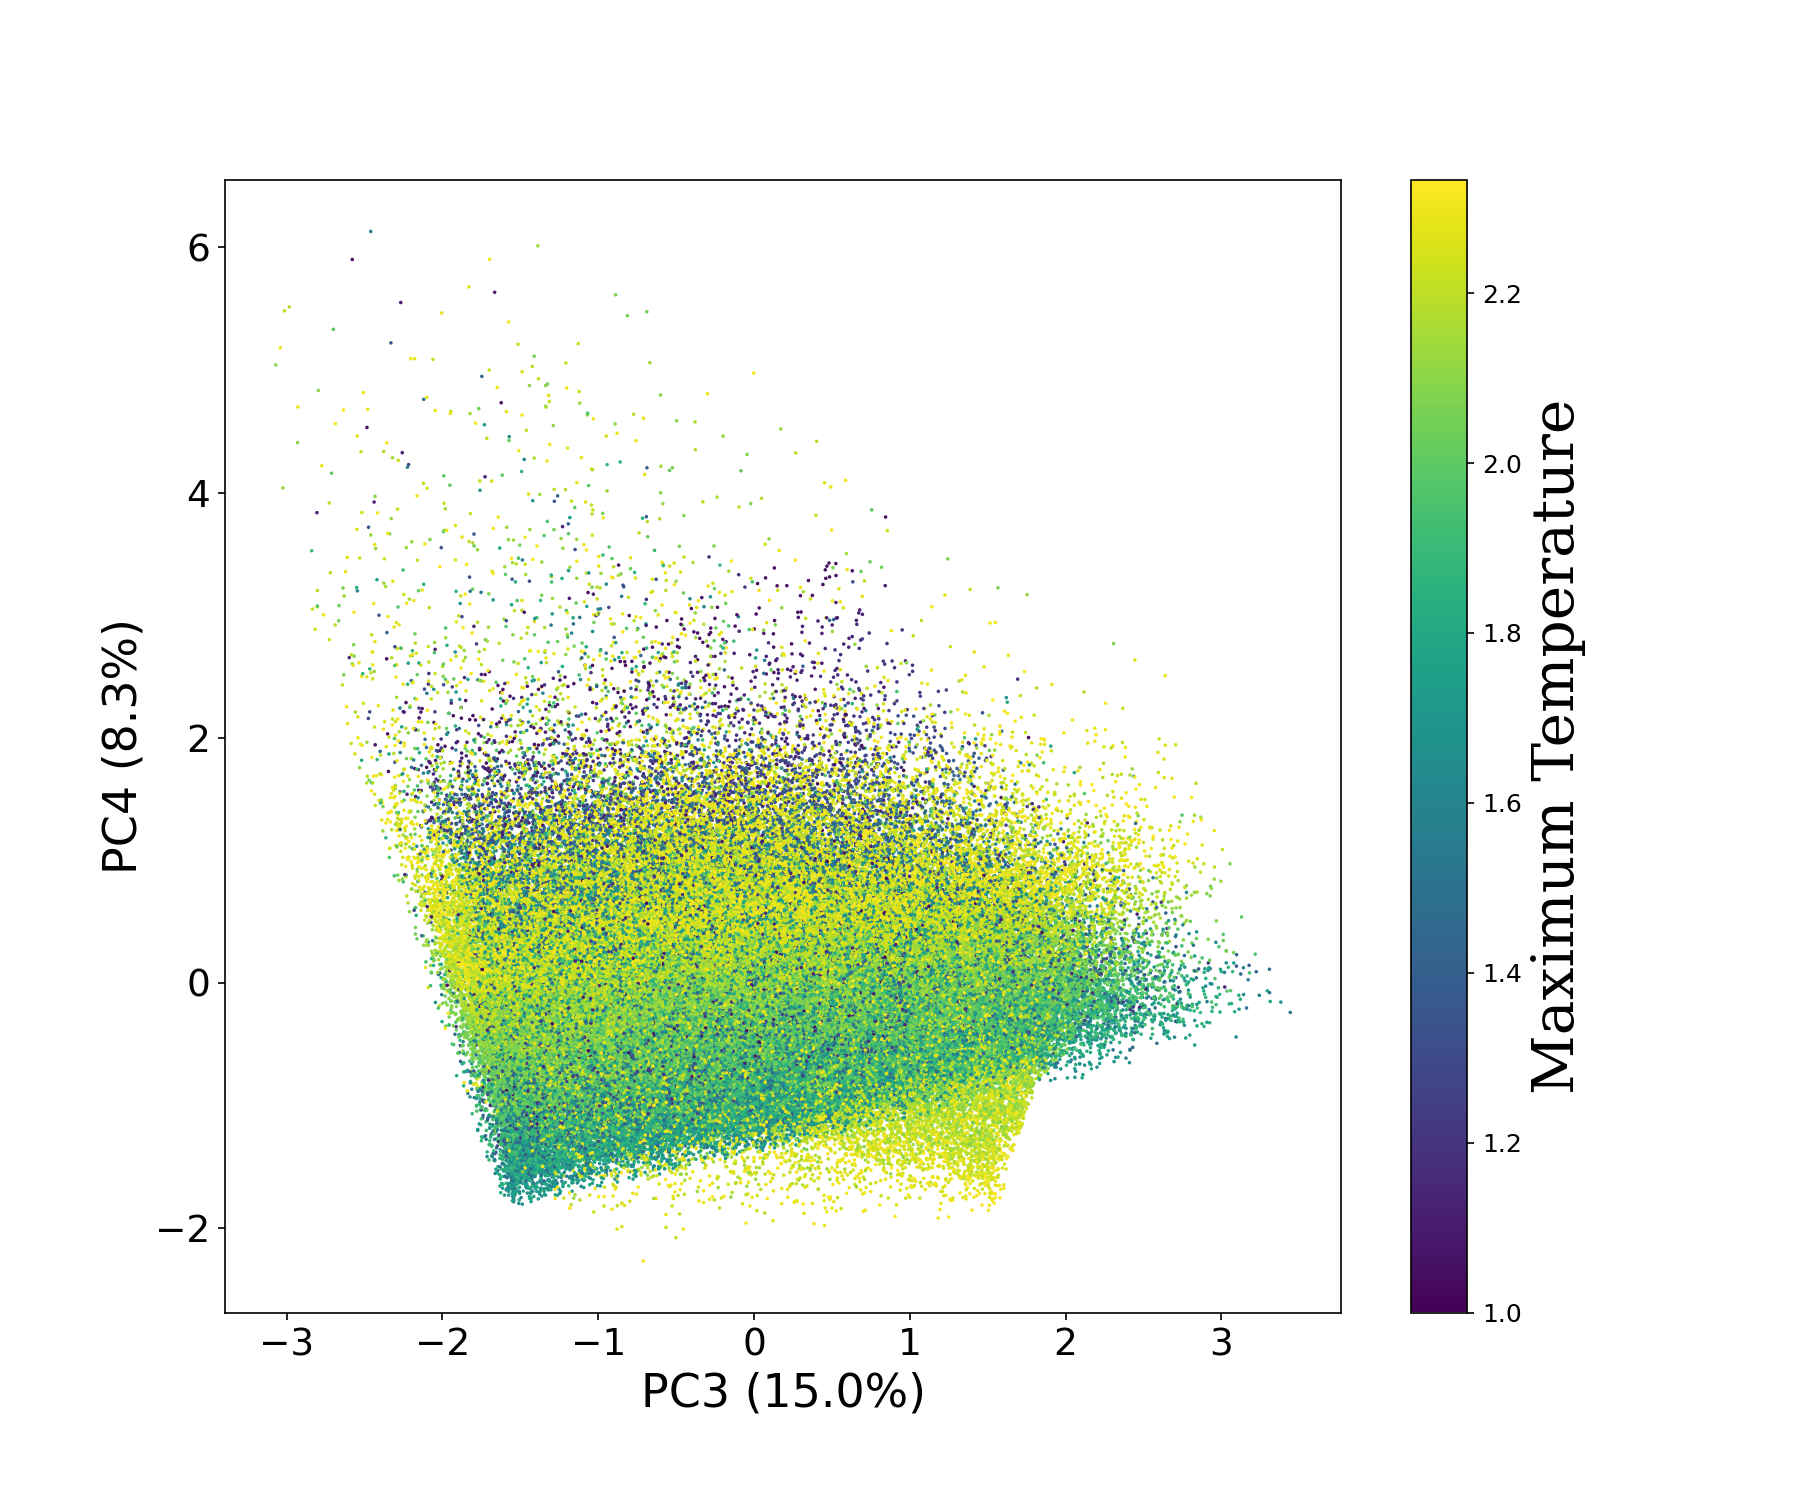
\includegraphics[width=5.9cm]{7/PC3&4_maxTemp.png}
} \\
\subfigure{
\label{C1-34-metallicity}
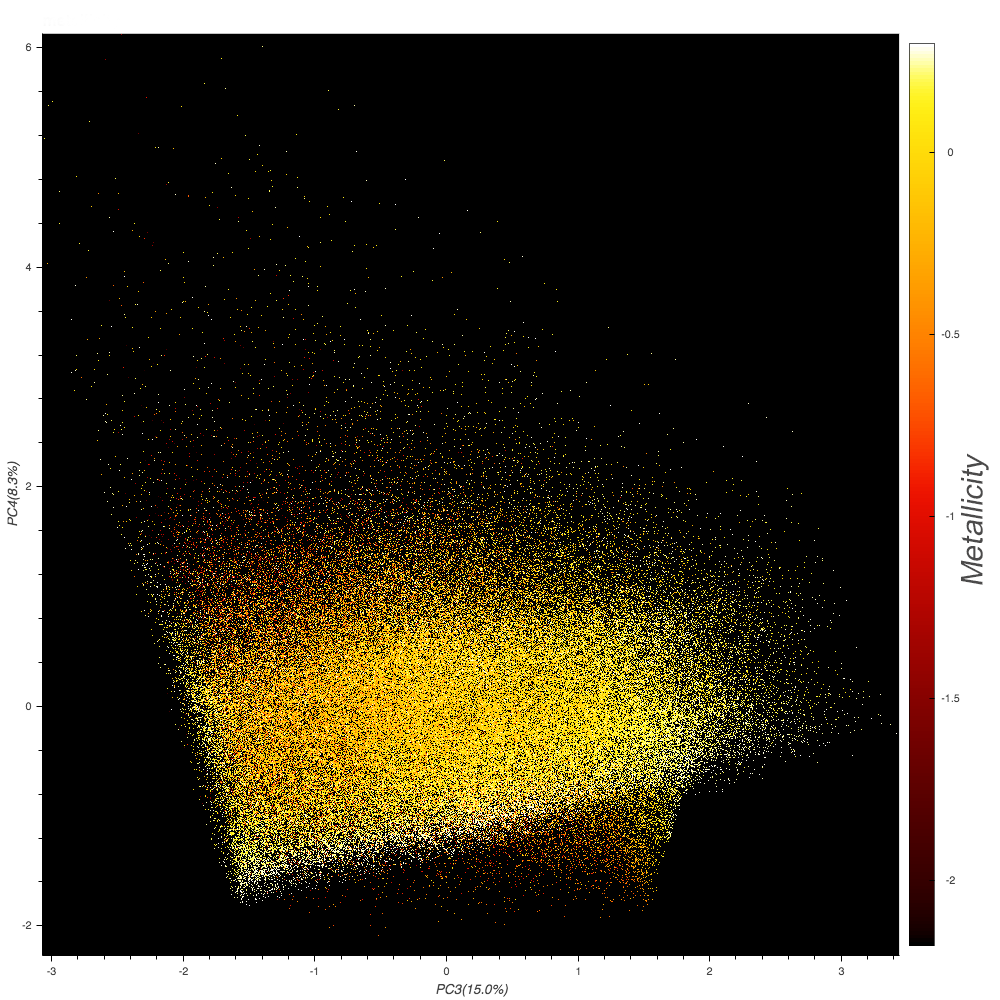
\includegraphics[width=5.9cm]{7/PC3&4_metallicity.png}
}
\subfigure{
\label{C1-34-radfield}
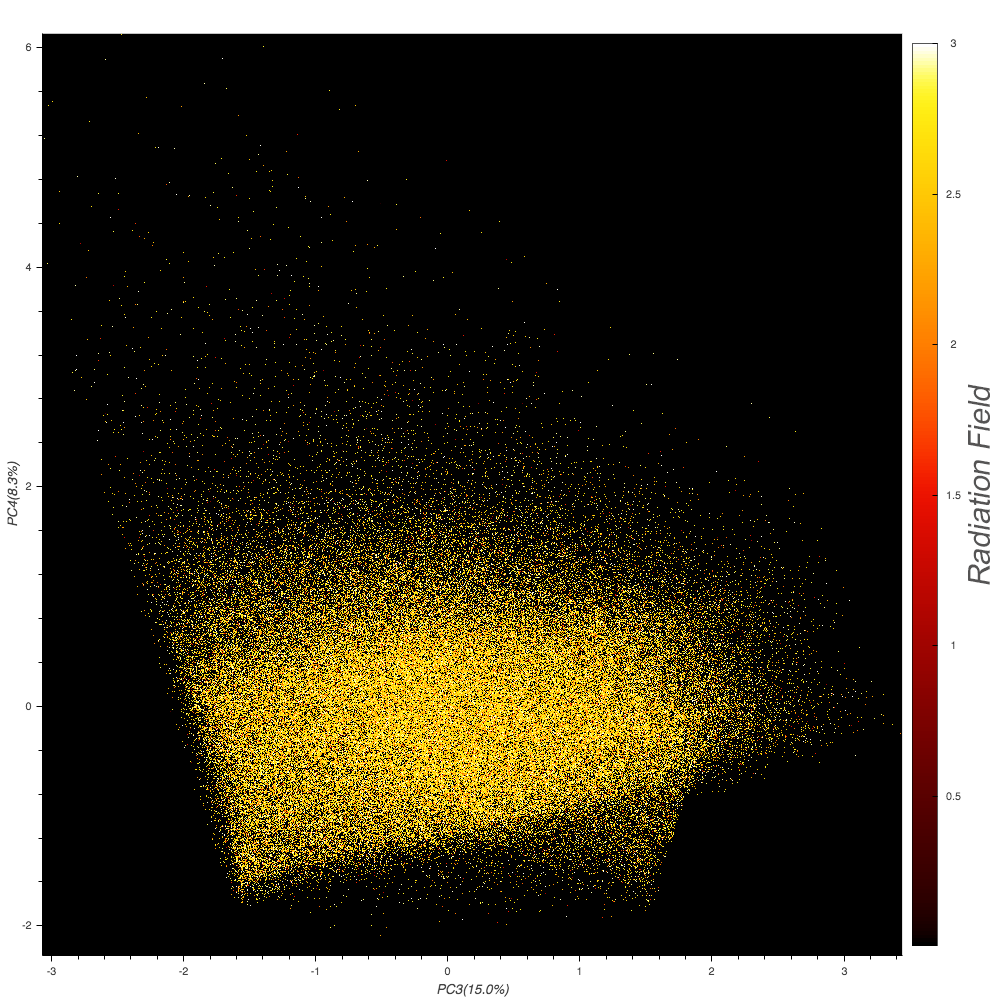
\includegraphics[width=5.9cm]{7/PC3&4_radfield.png}
}
\subfigure{
\label{C1-34-zeta}
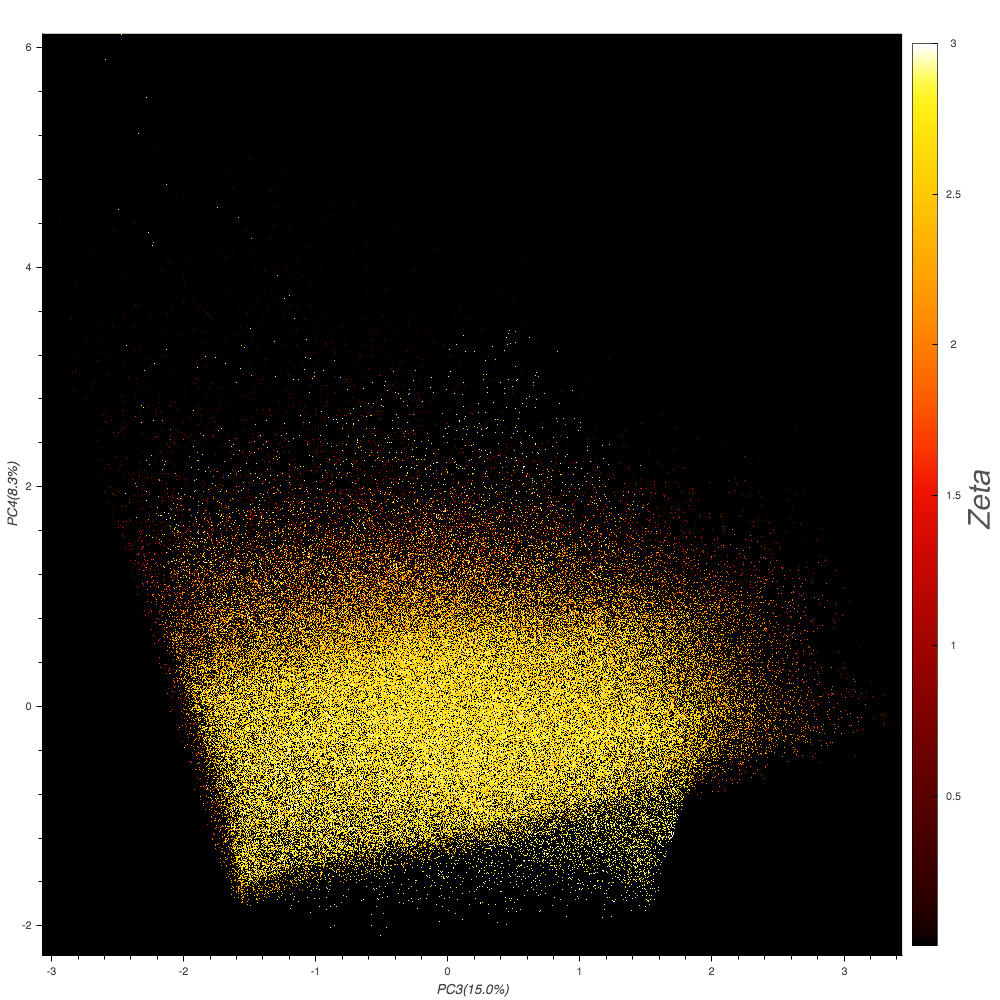
\includegraphics[width=5.9cm]{7/PC3&4_zeta.png}
}
\caption{Projection of Group C1 (CO, HCO$^+$, CS, SiO, HCN, NH$_3$, and HNC) on the plane of PC3 and PC4. Three panels on the top row are A\textsubscript{V}, initial densities and maximum temperature, while the three panels on the bottom row are metallicity, rad field and zeta, respectively. Among them, only the projection of initial densities and A\textsubscript{V} shows a clear trend.}
\label{C1-34}
\end{figure*}

  
  

   
   
   
      %%%%%---------------Table 3------------------------------

\begin{table*}[htbp]
\centering
\begin{tabular}{ccccc}
\hline\hline
\multirow{2}{*}{Principal Components} & \multicolumn{4}{c}{Physical Parameters}  \\ \cline{2-5} 
                                      & \begin{tabular}[c]{@{}c@{}}maximum \\ temperture\end{tabular} & \multicolumn{1}{l}{metallicity} & \multicolumn{1}{l}{A\textsubscript{V}} & \begin{tabular}[c]{@{}c@{}}initial\\ densities\end{tabular} \\ \hline
PC1 &  & -  & &  \\ \hline
PC2 & + & & &  \\ \hline
PC3 &   &   & +   & -   \\ \hline\hline
\end{tabular}
\caption{Changing trend of physical parameters on top three \\PCs among Group C1 (CO, HCO$^+$, CS, SiO, HCN, NH$_3$, and HNC).}
\label{table-7-all}
\end{table*}
  
  
   
   
\subsubsection{Group C2 (CO, HCO$^+$, CS, SiO, HCN, and HNC)}

  In this section, as NH$_3$ has been dropped, the subgroup of six molecules (CO, HCO$^+$, CS, SiO, HCN, and HNC) can be obtained to get to know the influence of NH$_3$ having on the whole group of molecules.
  Same as the procedure executed on the group of 7 molecules, the results of tables and figures are shown as follows. 
  Fig. \ref{Fig13} shows the individual and cumulative explained variance of 6 PCs. 
  Table \ref{table-6-variance} records the data of them. 
  Top three PCs consists of $87.4\%$ of the total variance: PC1 is $47.7\%$, PC2 is $23.3\%$, and PC3 is $16.5\%$. 
  
  
   %%%%%%------------   Figure 13------------------------ 
  \begin{figure}[htbp]
   \centering
   \captionsetup{justification=centering}
   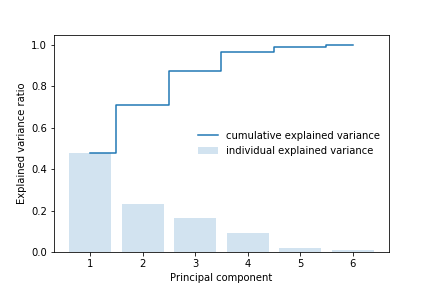
\includegraphics[angle=0,scale = 0.6]{6/explained_variance_ratio.png}
   \caption{Individual and cumulative explained variance of PCs among Group C2 (CO, HCO$^+$, CS, SiO, HCN, and HNC).}
         \label{Fig13}
   \end{figure}
   
   
   %%%%%%%------------- Table 4-----------------

\begin{table*}[htbp]
\centering
\begin{tabular}{ccc}
\hline\hline
\multicolumn{1}{l}{Pincipal Components} & \multicolumn{1}{l}{Explained Ratio} & Cumulative Variance \\ \hline
        PC1 & 0.477  & 0.477\\ 
        PC2 & 0.232  & 0.709\\
        PC3 & 0.165  & 0.874\\
        PC4 & 0.092  & 0.966\\ 
        PC5 & 0.021  & 0.987\\
        PC6 & 0.013  & 1.000\\ \hline\hline
\end{tabular}
\caption{Table of individual and cumulative explained variance of PCs among Group C2 (CO, HCO$^+$, CS, SiO, HCN, and HNC).}
\label{table-6-variance}
\end{table*}

  Fig. \ref{Fig-6-load-12}, Fig. \ref{Fig-6-load-23} and Table \ref{table-6-eigen} indicate the eigenvalues of molecular species having on PCs. On PC1, the molecule CO, HCN, and HNC contribute mostly, but are not that influential on PC2, where the HCO$^+$ and CS are the more significant ones. 
  On PC3, however, the SiO is the most crucial molecule, possessing an eigenvalue of 0.944. 
  Compared with the previous section, the same phenomenon can be also observed among seven molecules without dropping NH$_3$. 
  
 

%%%%%%%%%%---------------Table 5 -----------------
\begin{table*}[htp]
\centering
\begin{tabular}{ccccccc}
\hline\hline
\multirow{2}{*}{Molecular Species} & \multicolumn{6}{c}{Principal Components}                 \\ \cline{2-7} 
                                   & 1       & 2       & 3       & 4       & 5      & 6       \\ \hline
CO                                 & -0.570 & -0.112 & -0.024 & -0.084 & 0.00 & 0.808  \\ \hline
HCO$^+$                               & -0.021 & 0.725  & 0.109  & -0.673 & 0.087  & 0.018  \\ \hline
CS                                 & -0.290 & -0.607 & 0.043  & -0.646 & 0.012 & -0.355 \\ \hline
SiO                                & -0.110 & -0.016 & 0.979  & 0.152  & 0.066  & -0.035 \\ \hline
HCN                                & -0.537 & 0.244  & -0.046 & 0.171  & -0.718 & -0.322 \\ \hline
HNC                                & -0.537 & 0.178  & -0.157 & 0.262  & 0.687 & -0.337 \\ \hline\hline
\end{tabular}
\caption{Eigenvalues of PCA among Group C2 (CO, HCO$^+$, CS, SiO, HCN, and HNC)}
\label{table-6-eigen}
\end{table*}
   

  %%%%-------------Figure ------------------------------------------------
      \begin{figure}[htbp]
\centering  
\subfigure[Plane of PC1 and PC2]{
\label{Fig-6-load-12}
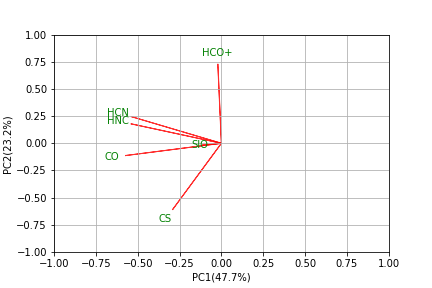
\includegraphics[width=0.5\textwidth]{6/loadingplot_PC1&2.png}}
\subfigure[Plane of PC2 and PC3]{
\label{Fig-6-load-23}
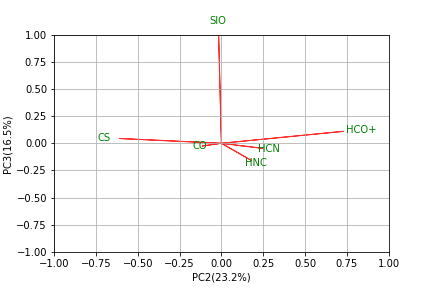
\includegraphics[width=0.5\textwidth]{6/loadingplot_PC2&3.png}}
\caption{Loading plots of Group C2 (CO, HCO$^+$, CS, SiO, HCN, and HNC)}
\label{Fig-6-load}
\end{figure}
   
   On the view of the projections of PCs, Fig. \ref{C2-12-maxtemp} and Fig. \ref{C2-23-maxtemp} indicate that the physical parameter maximum temperature contains an increasing trend along PC2. 
   Similarly, Fig. \ref{C2-23-av} and \ref{C2-34-av} shows that the physical parameter A\textsubscript{V} also has an upward tendency along the direction of PC3. 
   However, the physical parameter metallicity has a downward trend along the PC1, which can be observed in Fig. \ref{C2-12-metallicity}. Besides, the physical parameter initial densities also shows a decreasing trend along the PC3, which can be seen in Fig. \ref{C2-23-initialdens} and Fig. \ref{C2-34-initialdens}. 
   The same correspondence can be also found on Group C1. 
   Table \ref{table-6-all} records all of the obvious trends, where the positive and negative sign demonstrates the increasing and decreasing trend respectively. 
   
 %%%%----------------
\begin{figure*}[htbp]
\centering
\subfigure{
\label{C2-12-maxtemp}
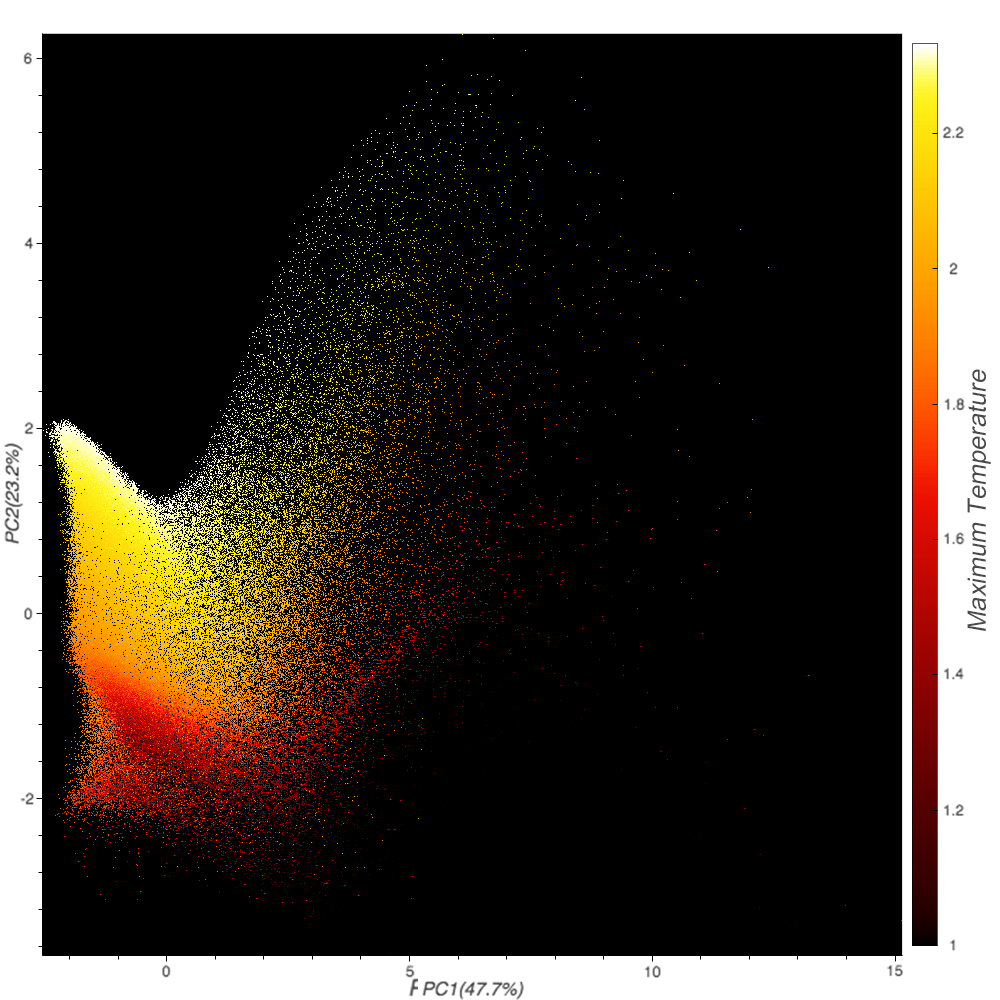
\includegraphics[width=5.9cm]{6/PC1&2_maxTemp.png}
}
\subfigure{
\label{C2-12-metallicity}
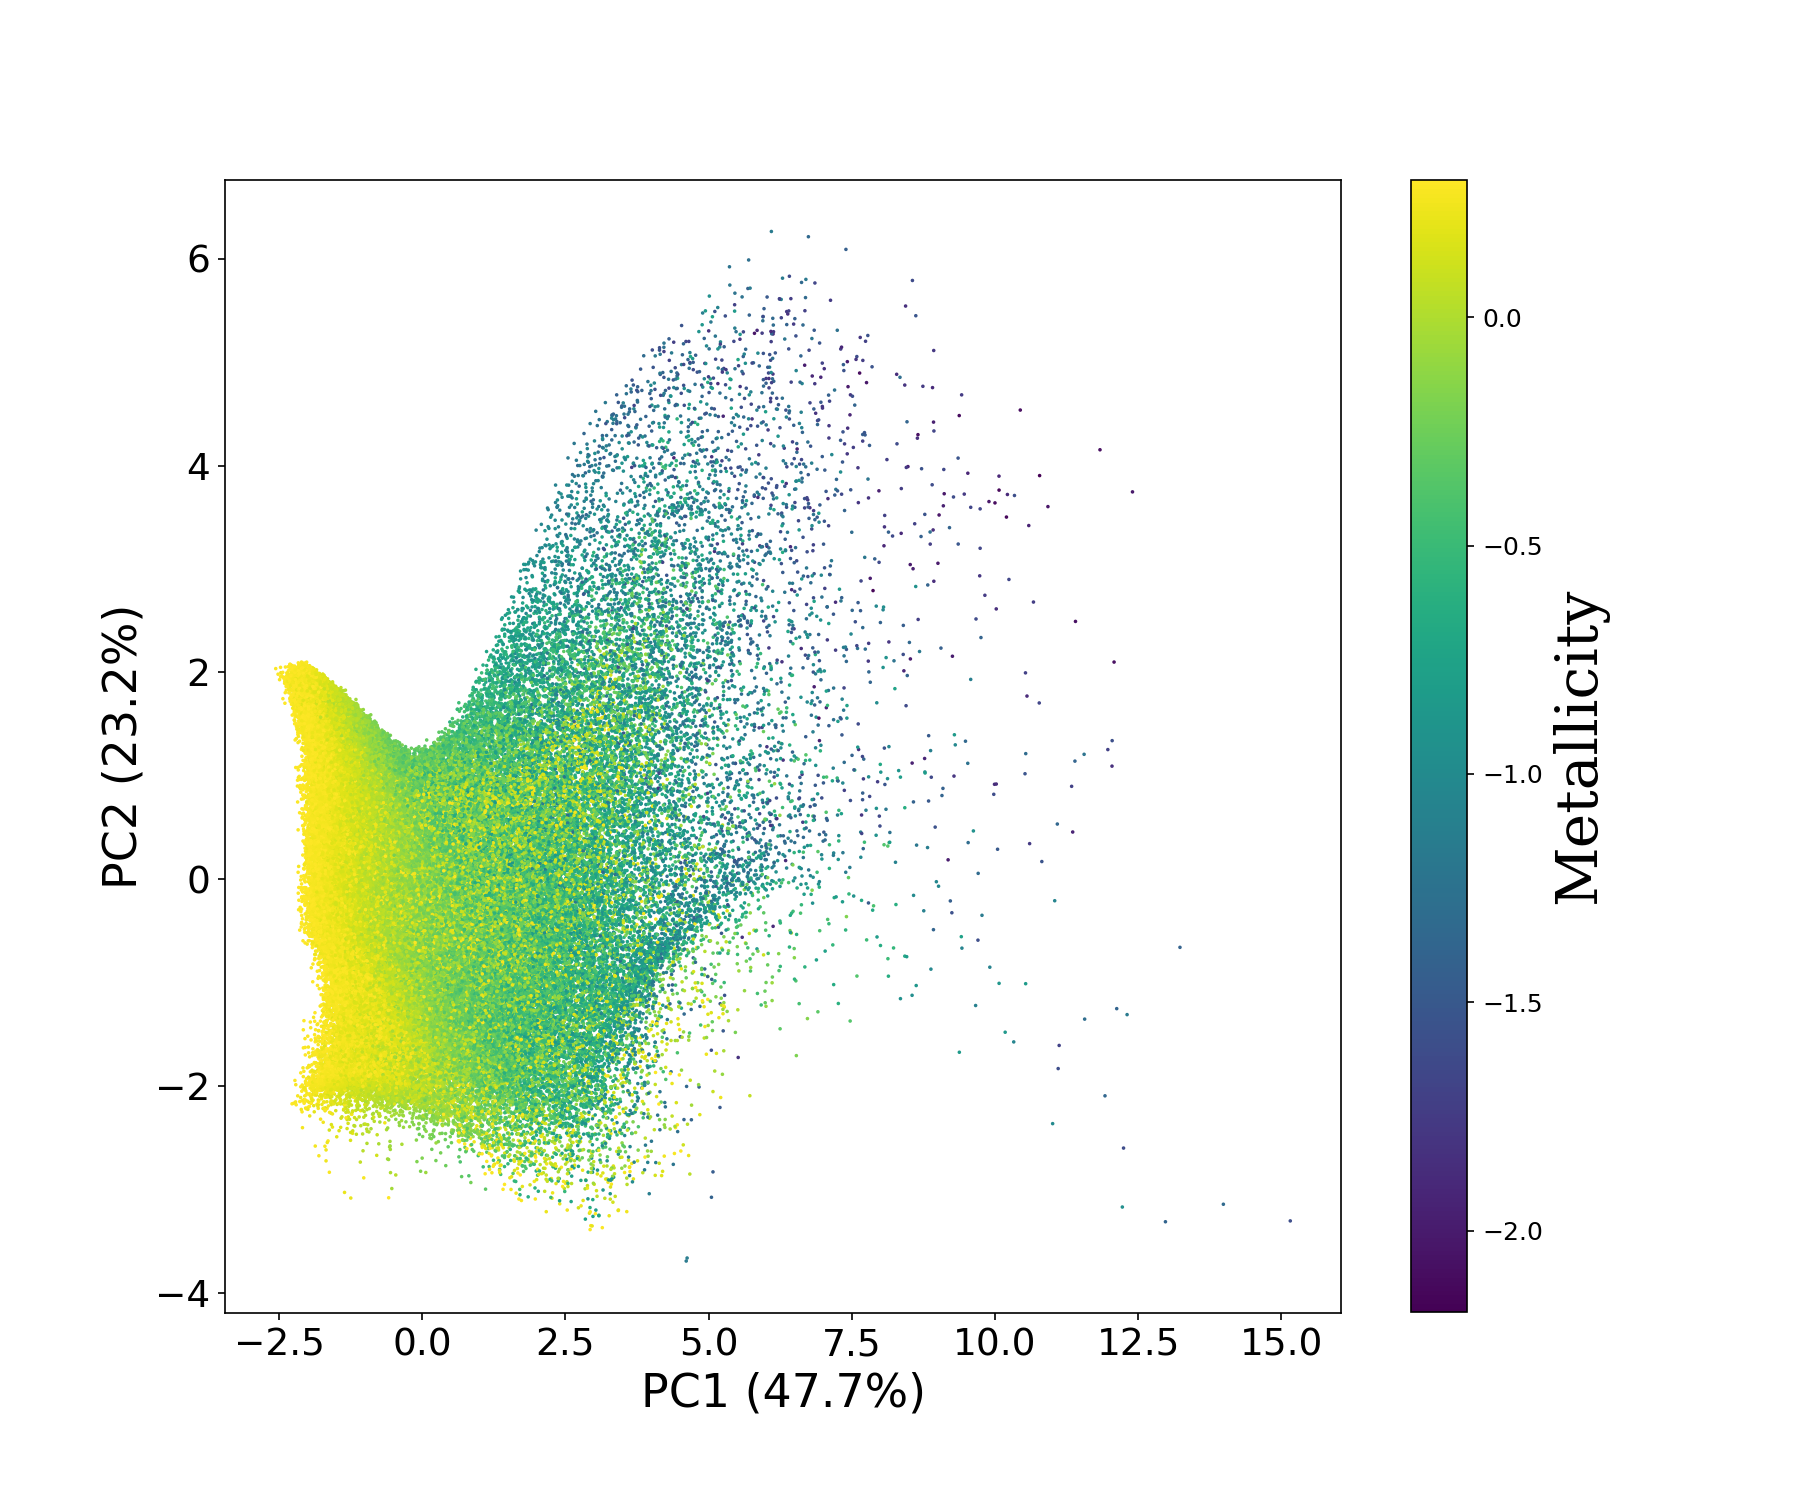
\includegraphics[width=5.9cm]{6/PC1&2_metallicity.png}
}
\caption{Projection of Group C2 (CO, HCO$^+$, CS, SiO, HCN, and HNC) on the plane of PC1 and PC2. The first panel is the maximum temperature, while the second panel demonstrates the metallicity.}
\label{C2-12}
\end{figure*}

 %%%%----------------------------------
\begin{figure*}[htbp]
\centering
\subfigure{
\label{C2-23-maxtemp}
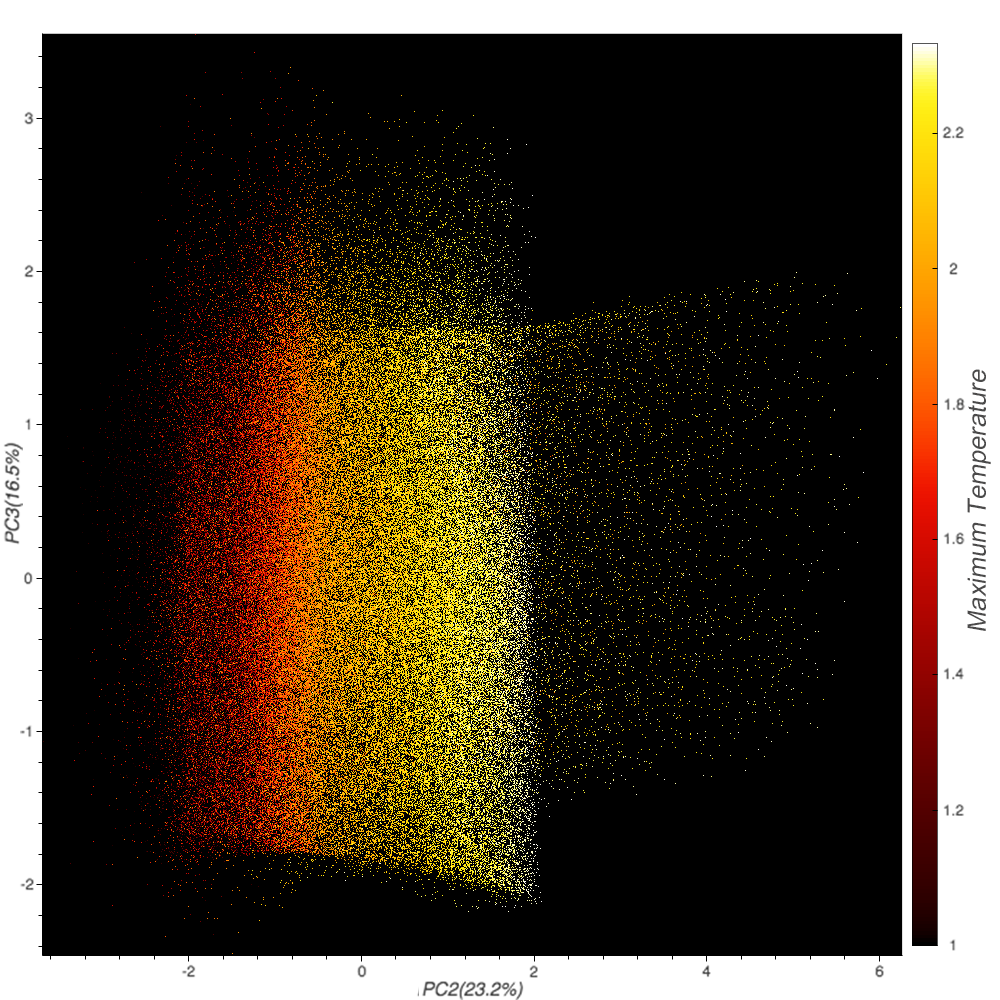
\includegraphics[width=5.9cm]{6/PC2&3_maxTemp.png}
} 
\subfigure{
\label{C2-23-metallicity}
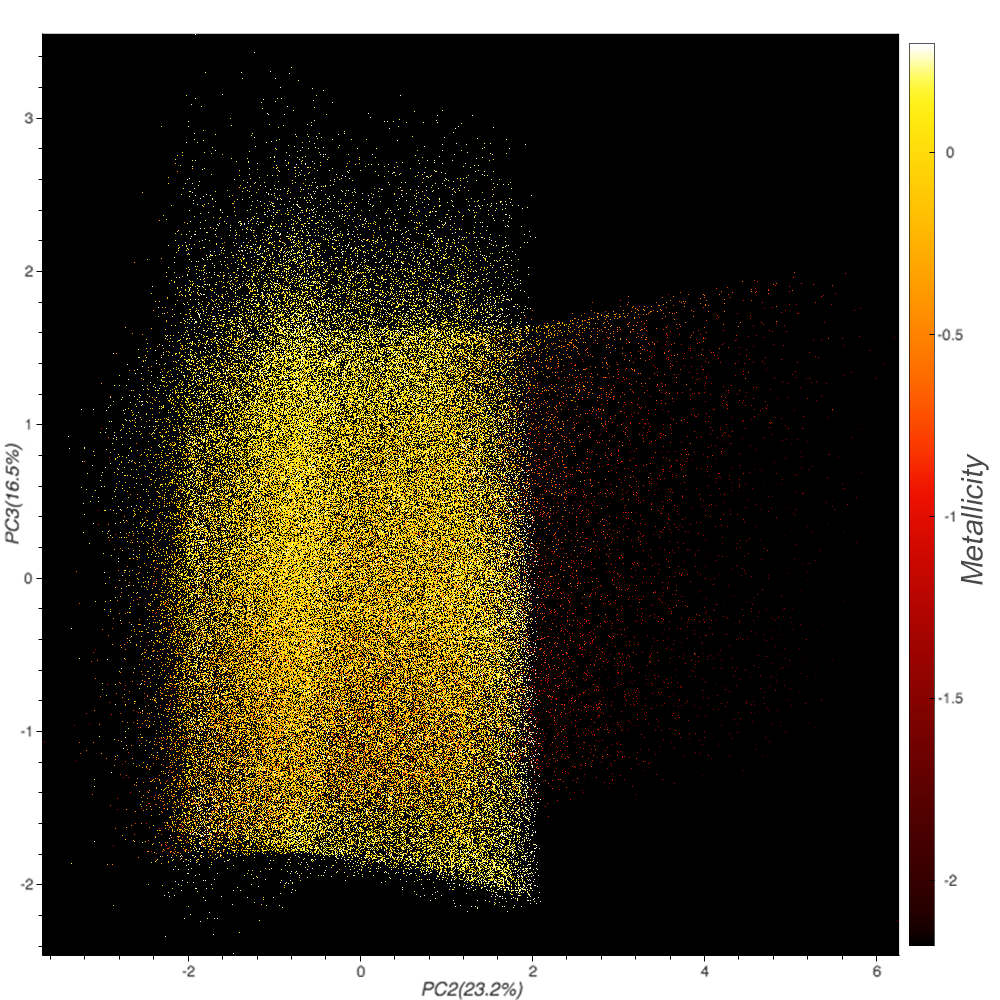
\includegraphics[width=5.9cm]{6/PC2&3_metallicity.png}
}
\\
\subfigure{
\label{C2-23-av}
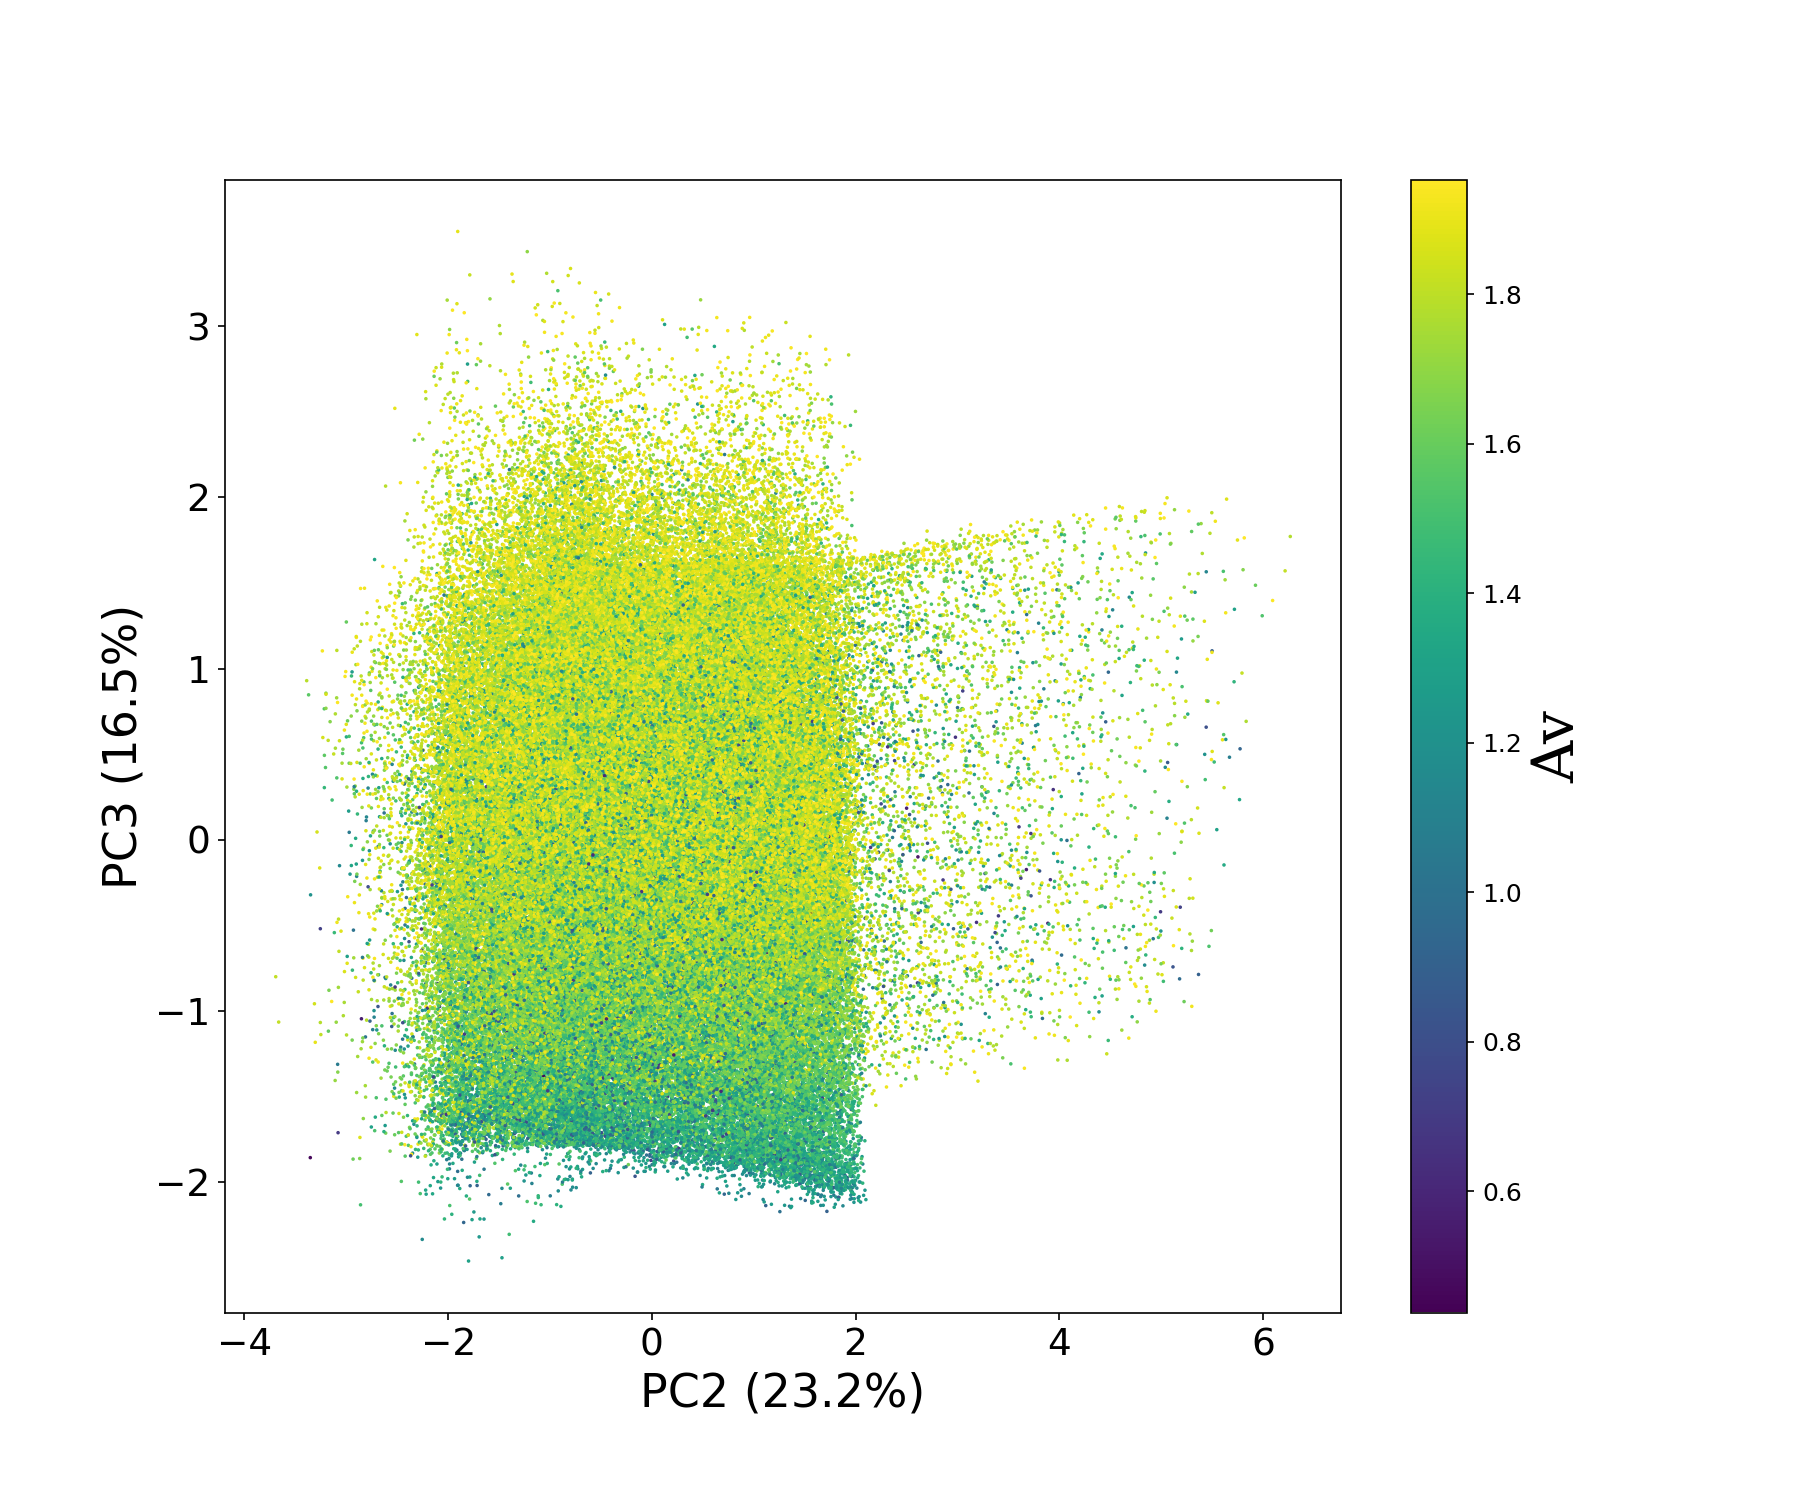
\includegraphics[width=5.9cm]{6/PC2&3_av.png}
}
\subfigure{
\label{C2-23-initialdens}
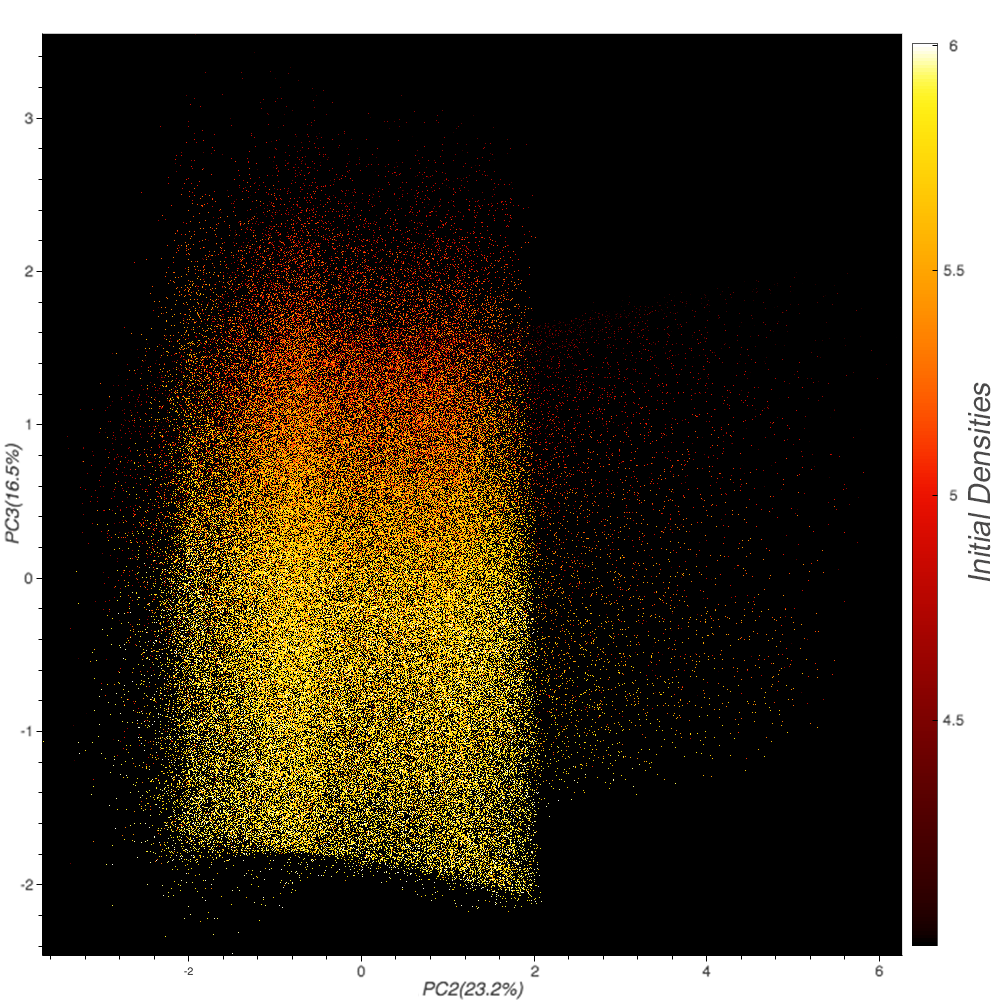
\includegraphics[width=5.9cm]{6/PC2&3_initialDens.png}
}
\caption{Projection of Group C2 (CO, HCO$^+$, CS, SiO, HCN, and HNC) on the plane of PC2 and PC3. The top row: max temperature and metallicity. The bottom row: A\textsubscript{V} and initial densities.}
\label{C2-23}
\end{figure*}
   
 %%%%-----------------------------------
\begin{figure*}[htbp]
\centering
\subfigure{
\label{C2-34-av}
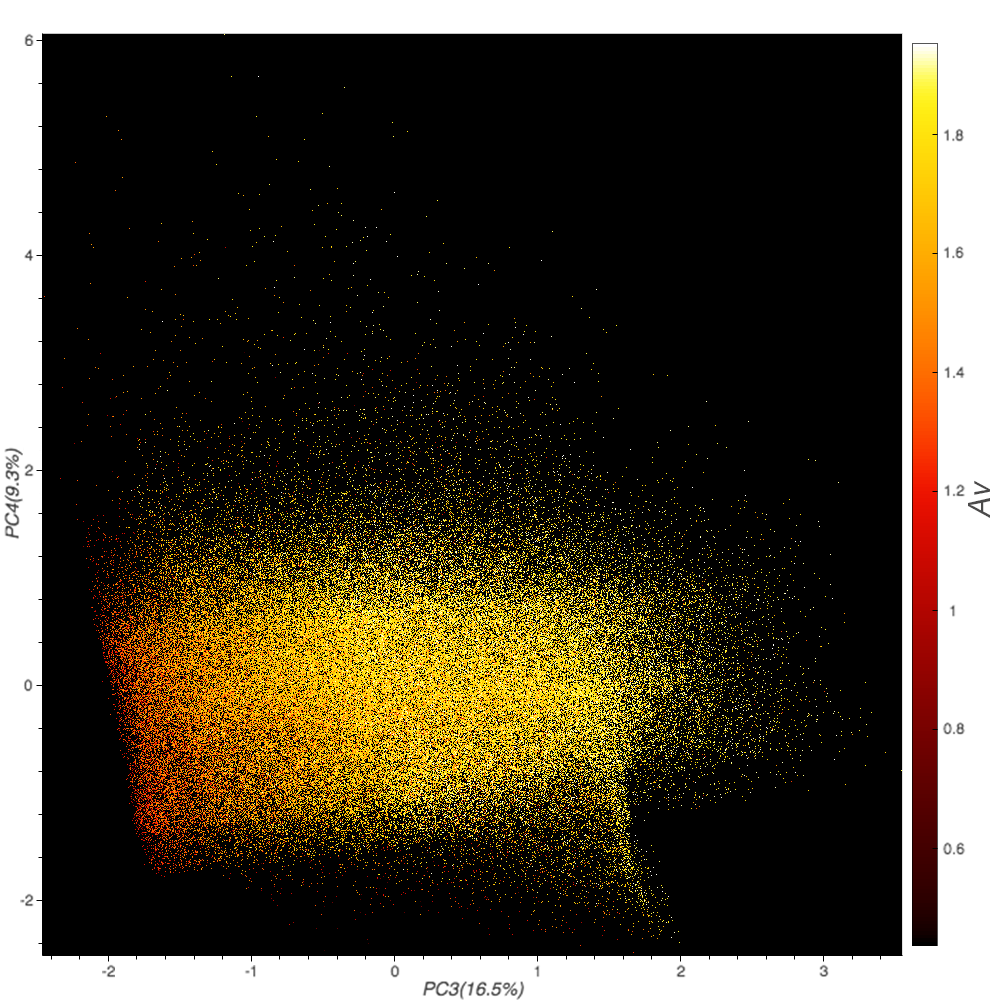
\includegraphics[width=5.9cm]{6/PC3&4_av.png}
}
\subfigure{
\label{C2-34-initialdens}
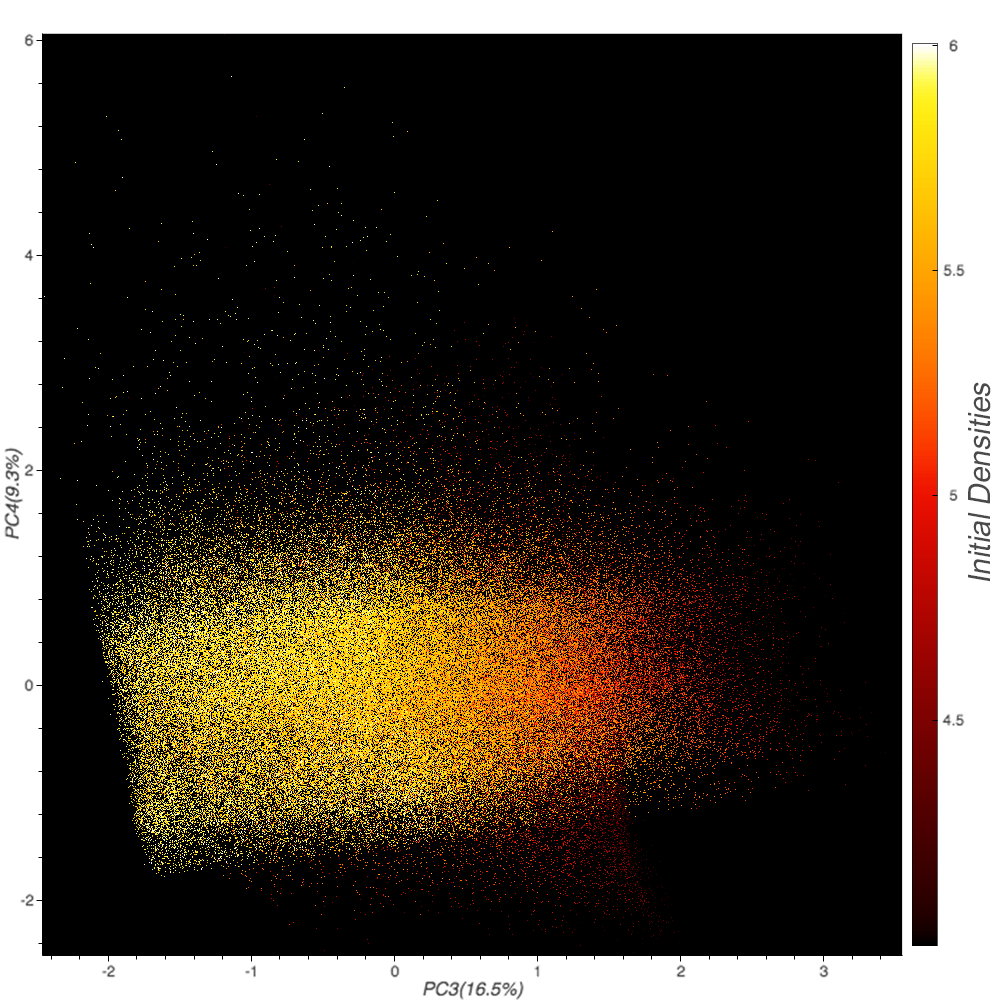
\includegraphics[width=5.9cm]{6/PC3&4_initialDens.png}
}
\caption{Projection of Group C2 (CO, HCO$^+$, CS, SiO, HCN, and HNC) on the plane of PC3 and PC4, demonstrating A\textsubscript{V} and initial densities respectively.}
\label{C2-34}
\end{figure*}

   %%%%%---------------Table 6------------------------------

  \begin{table*}[htbp]
  \centering
  \begin{tabular}{ccccc}
  \hline\hline
  \multirow{2}{*}{Principal Components} & \multicolumn{4}{c}{Physical Parameters}  \\ \cline{2-5} 
                                      & \begin{tabular}[c]{@{}c@{}}maximum \\ temperture\end{tabular} & \multicolumn{1}{l}{metallicity} & \multicolumn{1}{l}{A\textsubscript{V}} & \begin{tabular}[c]{@{}c@{}}initial\\ densities\end{tabular} \\ \hline
PC1 &  & -  & &  \\ \hline
PC2 & + & & &  \\ \hline
PC3 &   &   & +   & -   \\ \hline\hline
  \end{tabular}
  \caption{Changing trend of physical parameters on top three PCs among Group C2 (CO, HCO$^+$, CS, SiO, HCN, and HNC)}
  \label{table-6-all}
  \end{table*}
   
%%%%%%%%%-------------555555555555555555555555555555555555----------------------------------------
   
\subsubsection{Group C3 (CO, HCO$^+$, CS, SiO, and HCN)}

   Considering that the contribution of HCN and HNC are quite similar, we tried to cut down the number of molecules further by dropping one of them. 
   In this section, Group C3 contains only five molecules: CO, HCO$^+$, CS, SiO, and HCN. 
   As shown in Fig. \ref{Fig-5-variance} and Table \ref{table-5-variance}, the top three PCs are more clearly dominant, accounting for more than $95\%$ (PC1: $42.7\%$, PC2: $26.5\%$, PC3: $19.1\%$). 
   The loading plots in Fig. \ref{Fig-5-loading-12} and Fig. \ref{Fig-5-loading-23} as well as Table \ref{table-5-eigen} illustrate the eigenvalues of each molecule on PC1, PC2, and PC3, respectively. 
   On PC1, the molecule CO and HCN are influential. On PC2, the HCO$^+$ is the predominant one, possessing the eigenvalue of -0.772, where the minus indicates the opposite direction of PC2. 
   Fig. \ref{C3-12-maxtemp} and Fig. \ref{C3-23-maxtemp} reveal that the maximum temperature goes down along the direction of PC2. 
   Also for the metallicity, it decreases on the PC1, showing in Fig. \ref{C3-12-metallicity} and Fig. \ref{C3-23-metallicity}. 
   The physical parameter A\textsubscript{V} contains an increasing trend on PC3, as shown in Fig. \ref{C3-23-av} and Fig. \ref{C3-34-av}. 
   On the contrary, the initial densities has an decreasing trend on PC3, which can be observed on and Fig. \ref{C3-23-initialdens} and Fig. \ref{C3-34-initialdens}. 
   These trends are listed in Table \ref{table-5-all}. 
   
   %%%%%%------------   Figure 24------------------------ 
  \begin{figure}[htbp]
   \centering
   \captionsetup{justification=centering}
   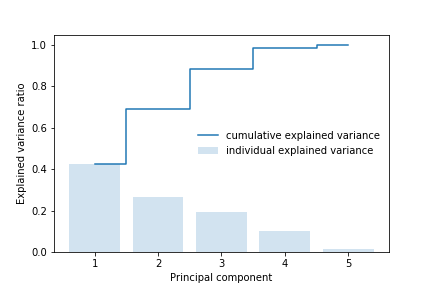
\includegraphics[angle=0,scale = 0.6]{5/explained_variance_ratio.png}
   \caption{Individual and cumulative explained variance of PCs among Group C3 (CO, HCO$^+$, CS, SiO, and HCN)}
         \label{Fig-5-variance}
   \end{figure}
   
%%%%%%%------------- Table 7-----------------

\begin{table*}[htbp]
\centering
\begin{tabular}{ccc}
\hline\hline
\multicolumn{1}{l}{Principal Components} & \multicolumn{1}{l}{Explained Ratio} & Cumulative Variance \\ \hline
        PC1 & 0.427  & 0.427\\ 
        PC2 & 0.265  & 0.692\\
        PC3 & 0.191  & 0.883\\
        PC4 & 0.101  & 0.984\\ 
        PC5 & 0.016  & 1.000\\ \hline\hline
\end{tabular}
\caption{Table of individual and cumulative explained variance of PCs among Group C3 (CO, HCO$^+$, CS, SiO, and HCN)}
\label{table-5-variance}
\end{table*}


   %%%------------Figure -----
   \begin{figure}[htbp]
\centering  
\subfigure[Plane of PC1 and PC2]{
\label{Fig-5-loading-12}
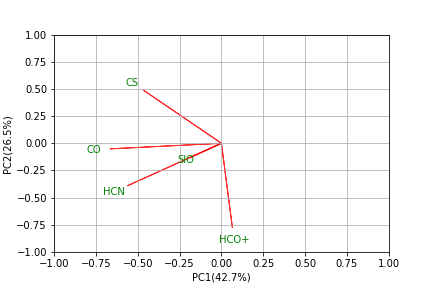
\includegraphics[width=0.5\textwidth]{5/loadingplot_PC1&2.png}}
\subfigure[Plane of PC2 and PC3]{
\label{Fig-5-loading-23}
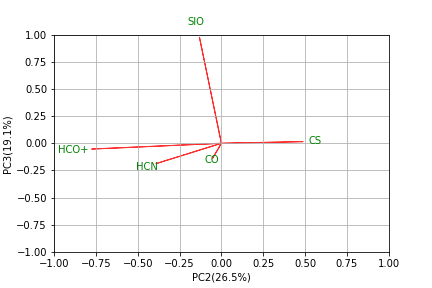
\includegraphics[width=0.5\textwidth]{5/loadingplot_PC2&3.png}}
\caption{Loading plots of Group C3 (CO, HCO$^+$, CS, SiO, and HCN)}
\label{Fig-5-loading}
\end{figure}
   
%%%%%%%%%----------Table 8---------------
\begin{table*}[htbp]
\centering
\begin{tabular}{cccccc}
\hline\hline
\multirow{2}{*}{Molecular Species} & \multicolumn{5}{c}{Principal Components}                 \\ \cline{2-6} 
                                   & 1       & 2       & 3       & 4       & 5 \\ \hline
CO   & -0.661 & -0.051  & -0.133 & 0.059  & 0.734 \\ \hline
HCO$^+$ & 0.065  & -0.771 & -0.052 & -0.629  & 0.046 \\ \hline
CS   & -0.461 & 0.484  & 0.015   & -0.667 & -0.326\\ \hline
SiO  & -0.186 & -0.130 & 0.971  & 0.058  & -0.005\\ \hline
HCN  & -0.556 & -0.387 & -0.185 & 0.389  & -0.594\\ \hline\hline
\end{tabular}
\caption{Eigenvalues of PCA among Group C3 (CO, HCO$^+$, CS, SiO, and HCN)} 
\label{table-5-eigen}
\end{table*}

 %%%%------------------------------------------
\begin{figure*}[htbp]
\centering
\subfigure{
\label{C3-12-maxtemp}
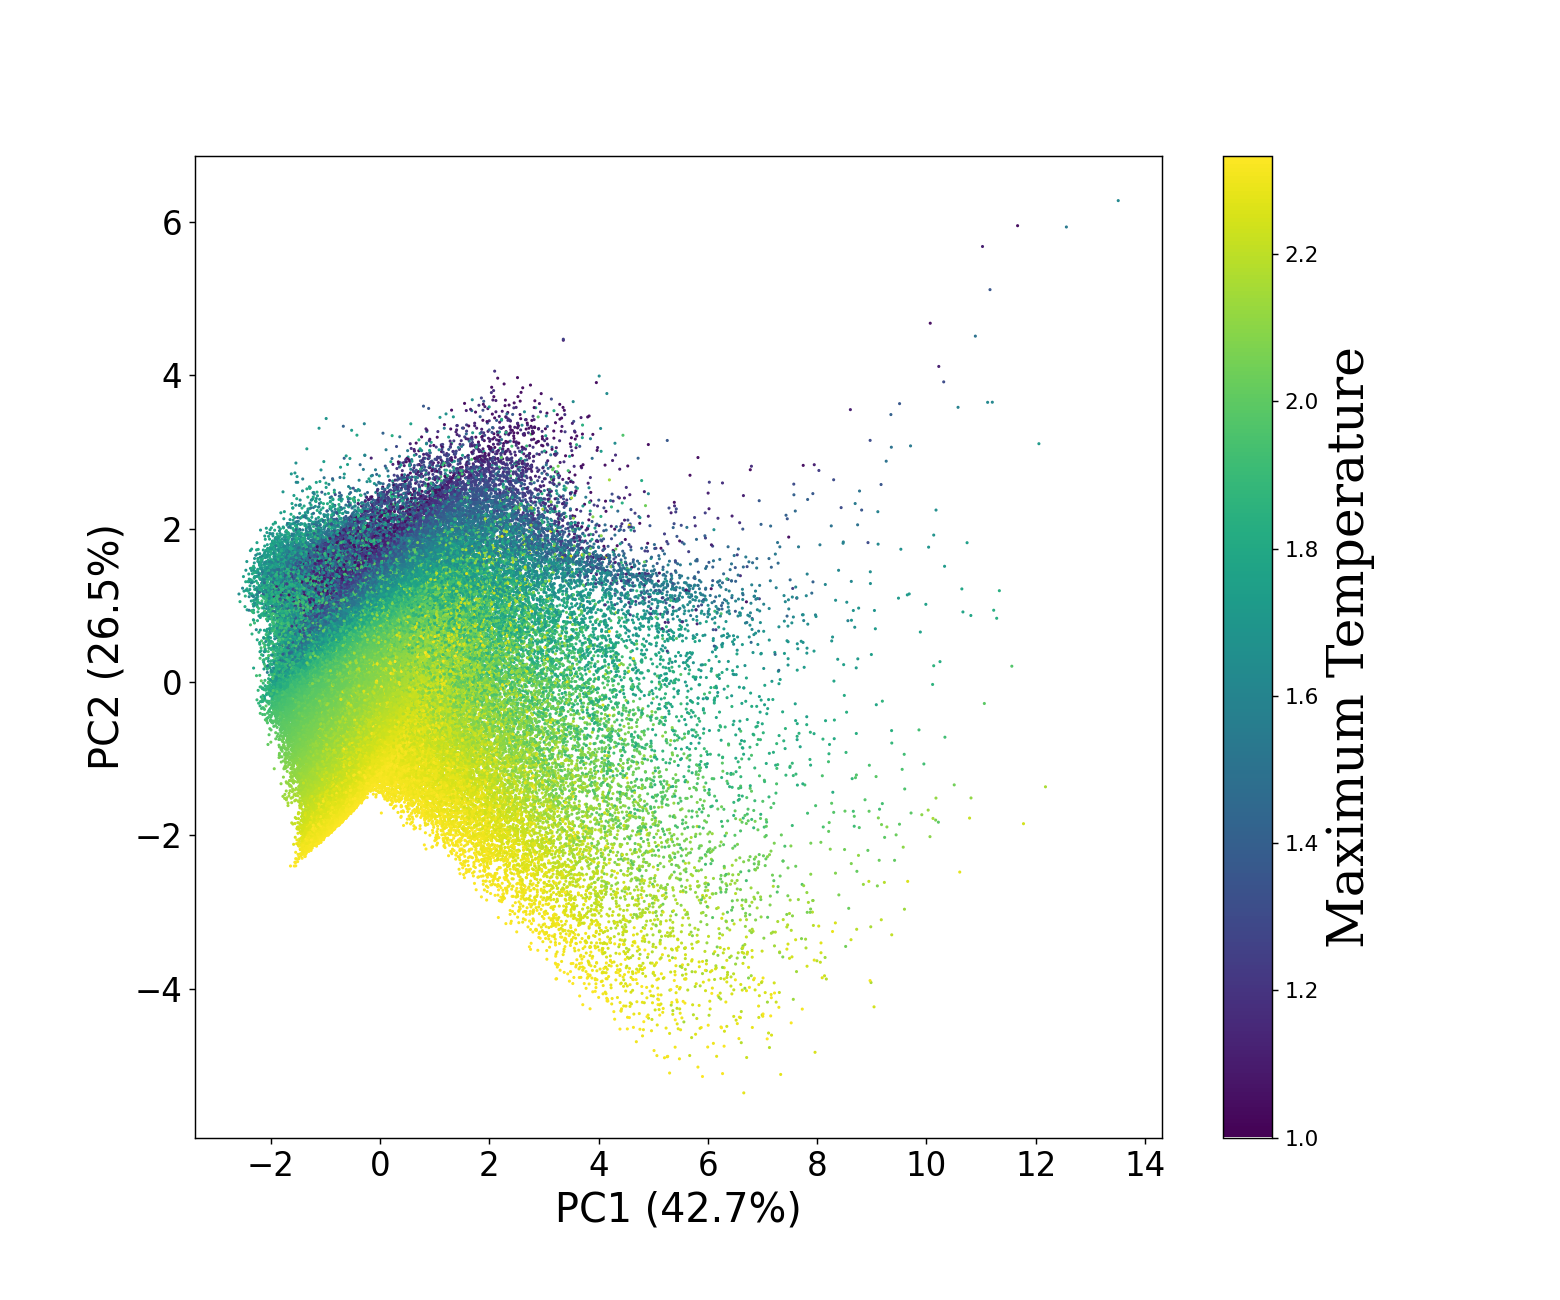
\includegraphics[width=5.9cm]{5/PC1&2_maxTemp.png}
}
\subfigure{
\label{C3-12-metallicity}
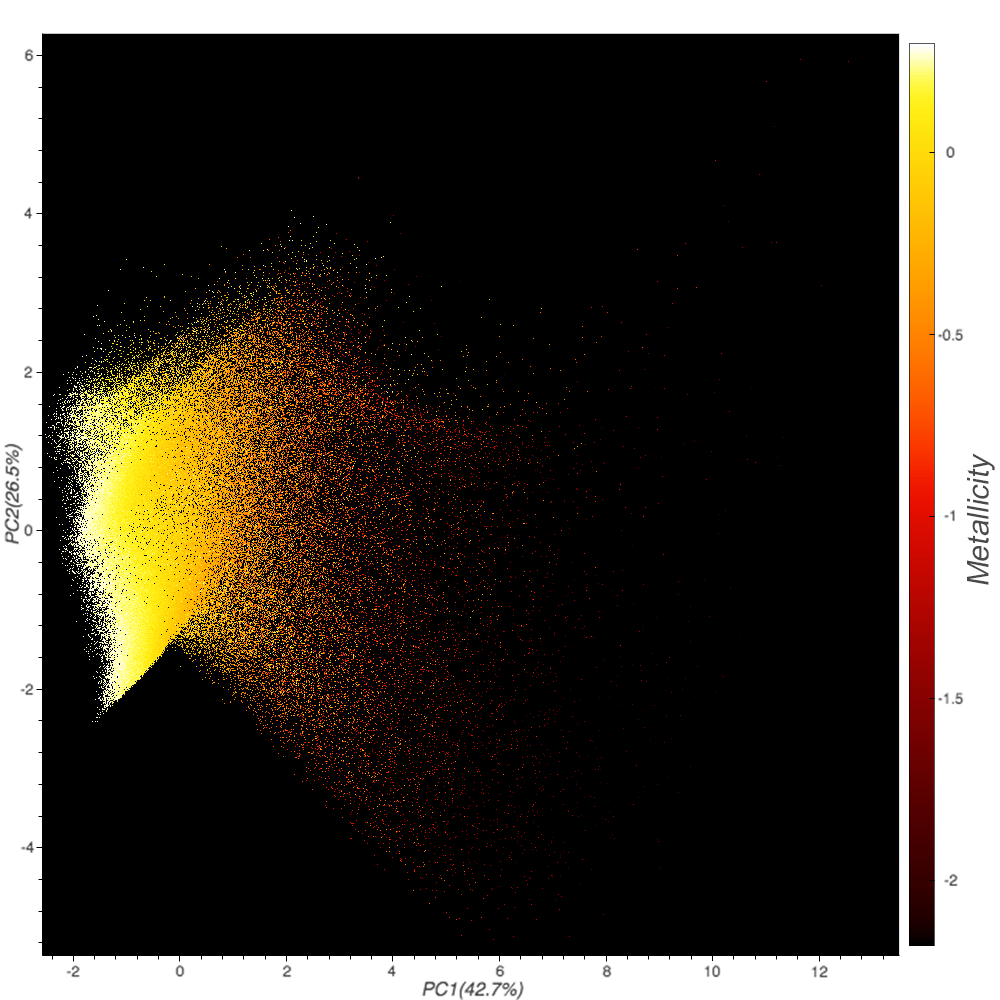
\includegraphics[width=5.9cm]{5/PC1&2_metallicity.png}
}
\caption{Projection of Group C3 (CO, HCO$^+$, CS, SiO, and HCN) on the plane of PC1 and PC2. The first panel is the maximum temperature, while the second panel demonstrates the metallicity.}
\label{C3-12}
\end{figure*}

 %%%%-------------------------------------------
\begin{figure*}[htbp]
\centering
\subfigure{
\label{C3-23-maxtemp}
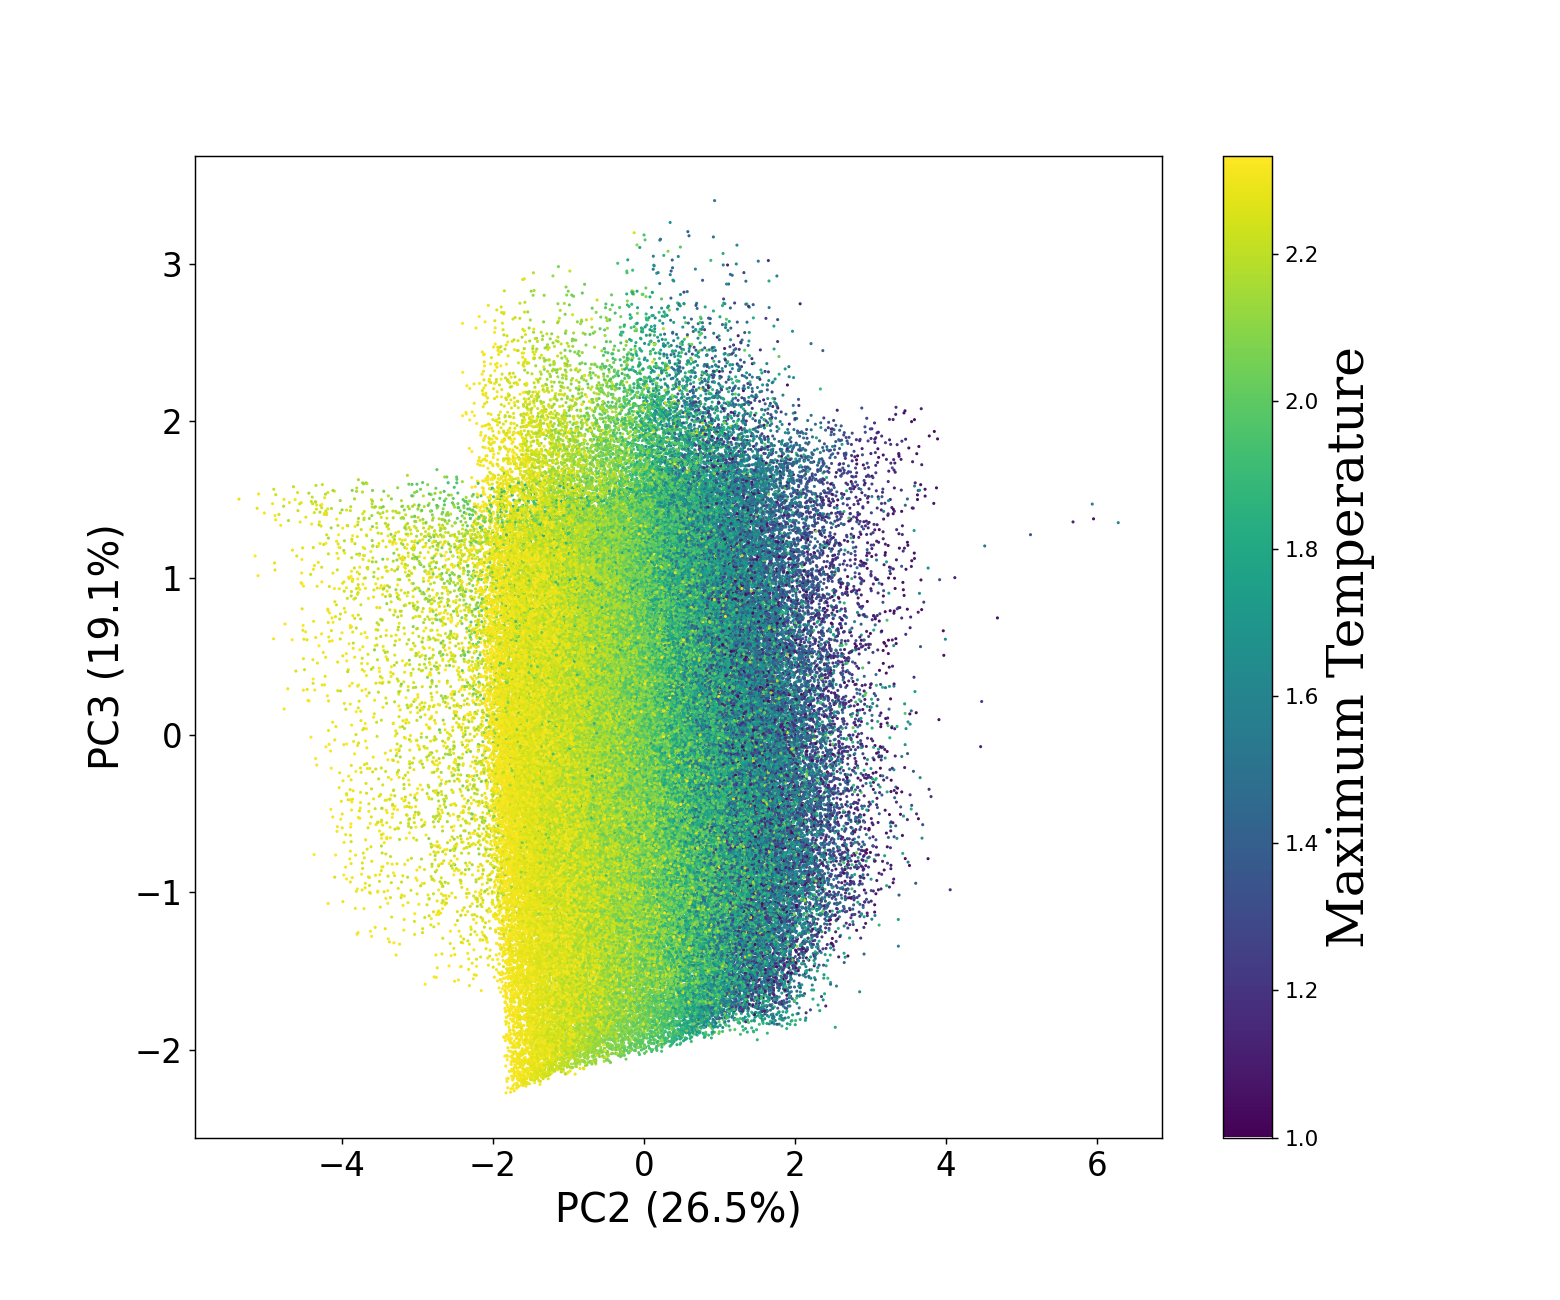
\includegraphics[width=5.9cm]{5/PC2&3_maxTemp.png}
} 
\subfigure{
\label{C3-23-metallicity}
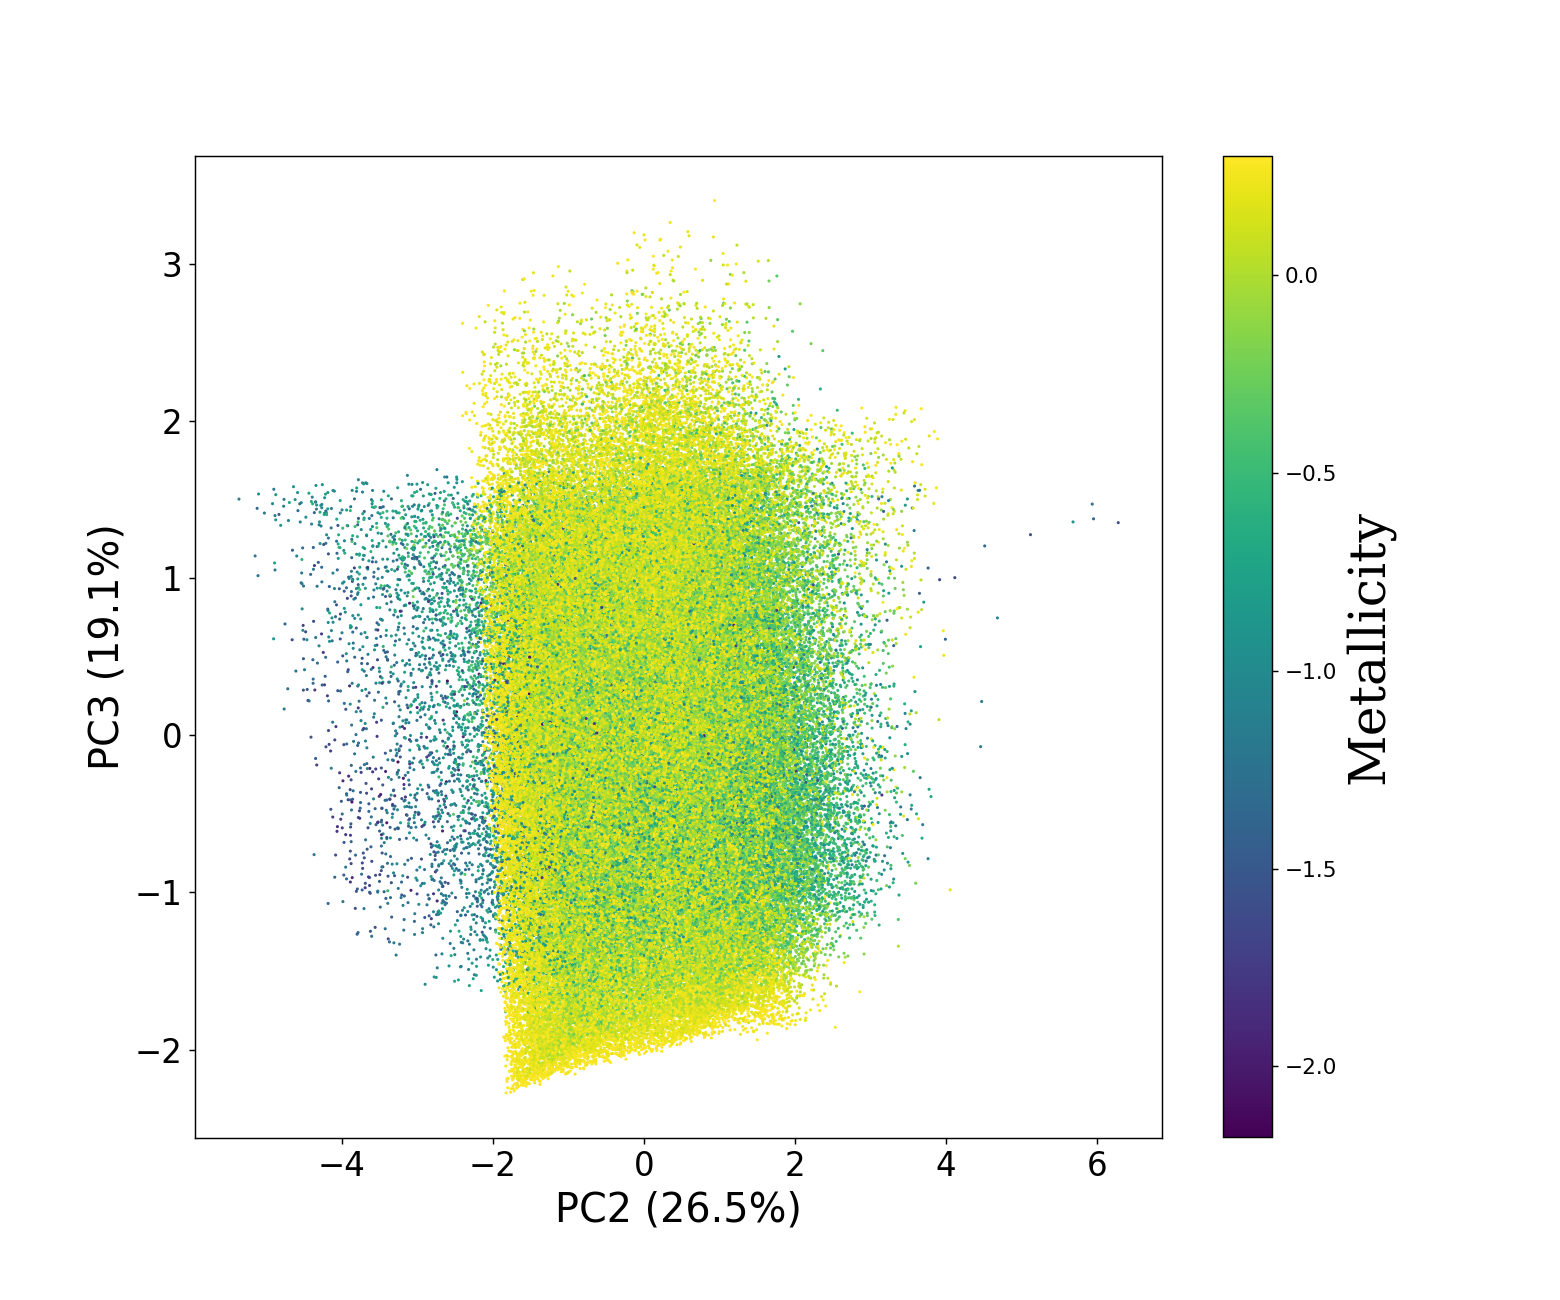
\includegraphics[width=5.9cm]{5/PC2&3_metallicity.png}
}
\\
\subfigure{
\label{C3-23-av}
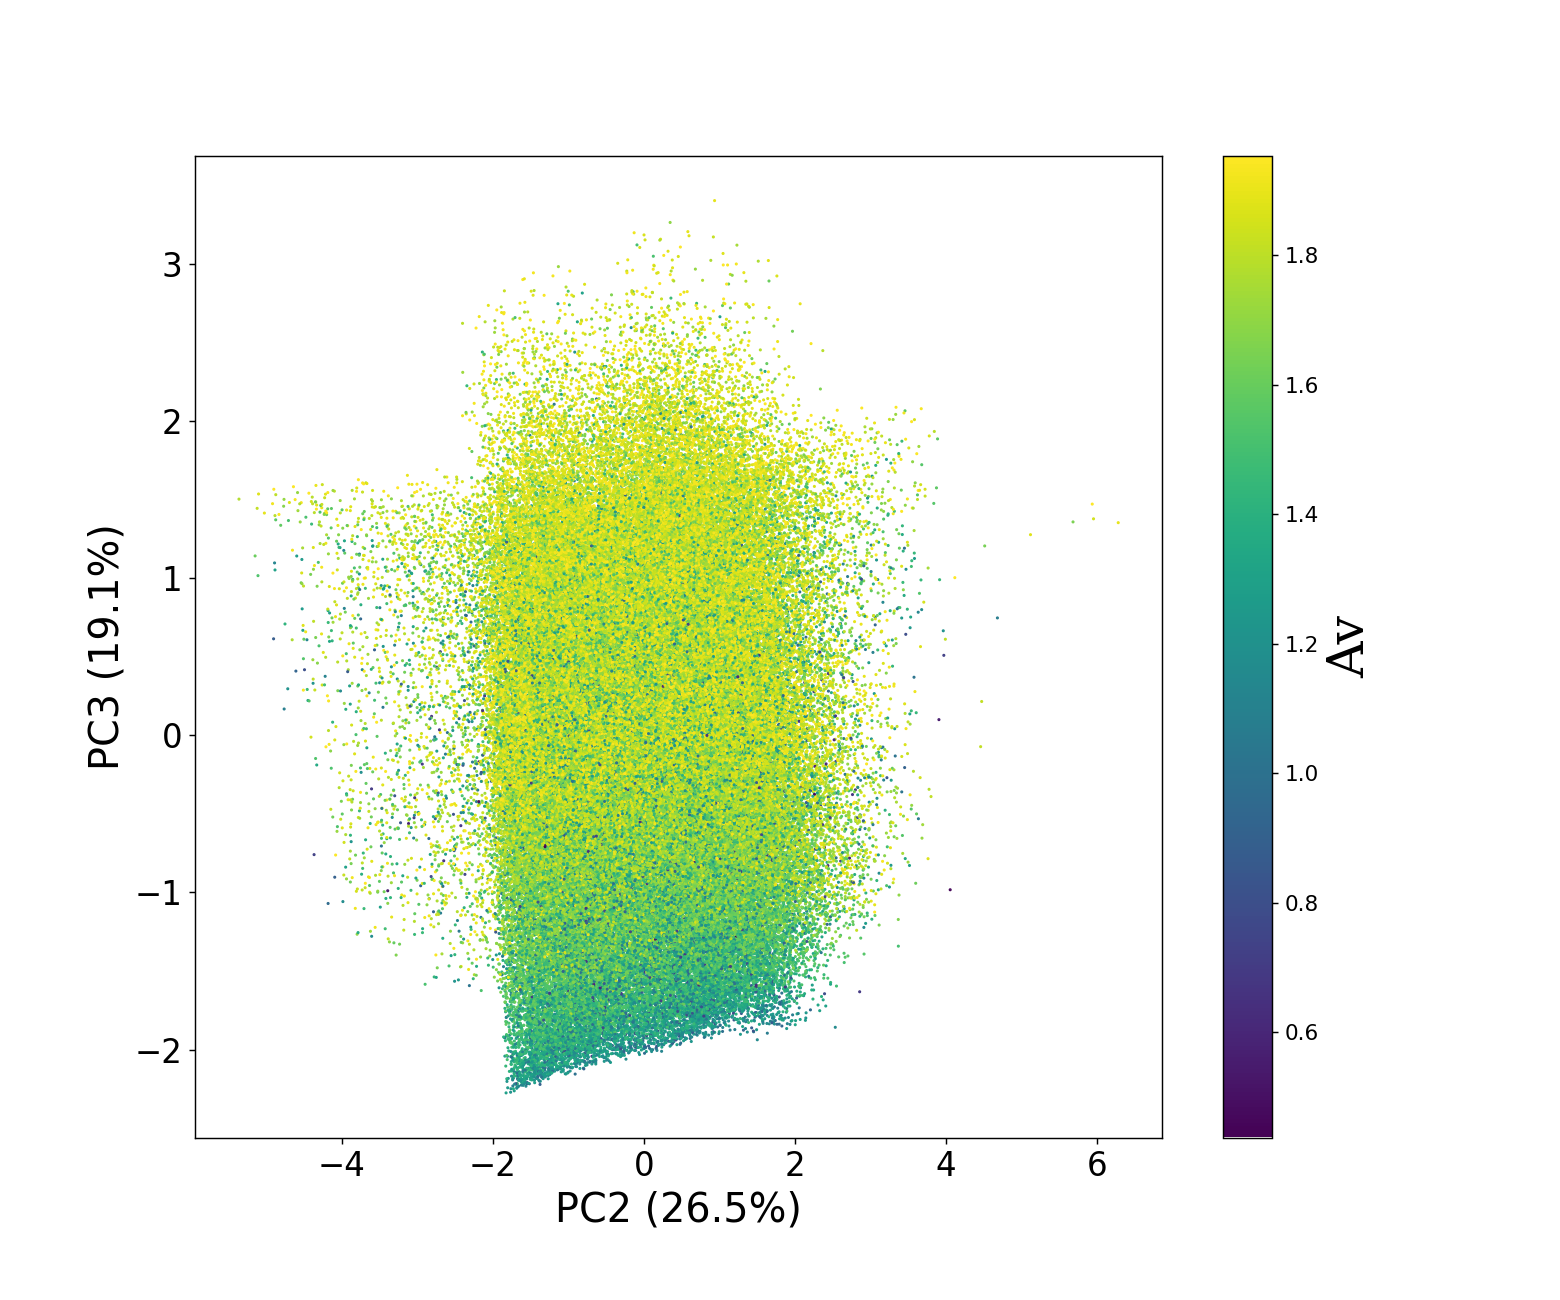
\includegraphics[width=5.9cm]{5/PC2&3_av.png}
}
\subfigure{
\label{C3-23-initialdens}
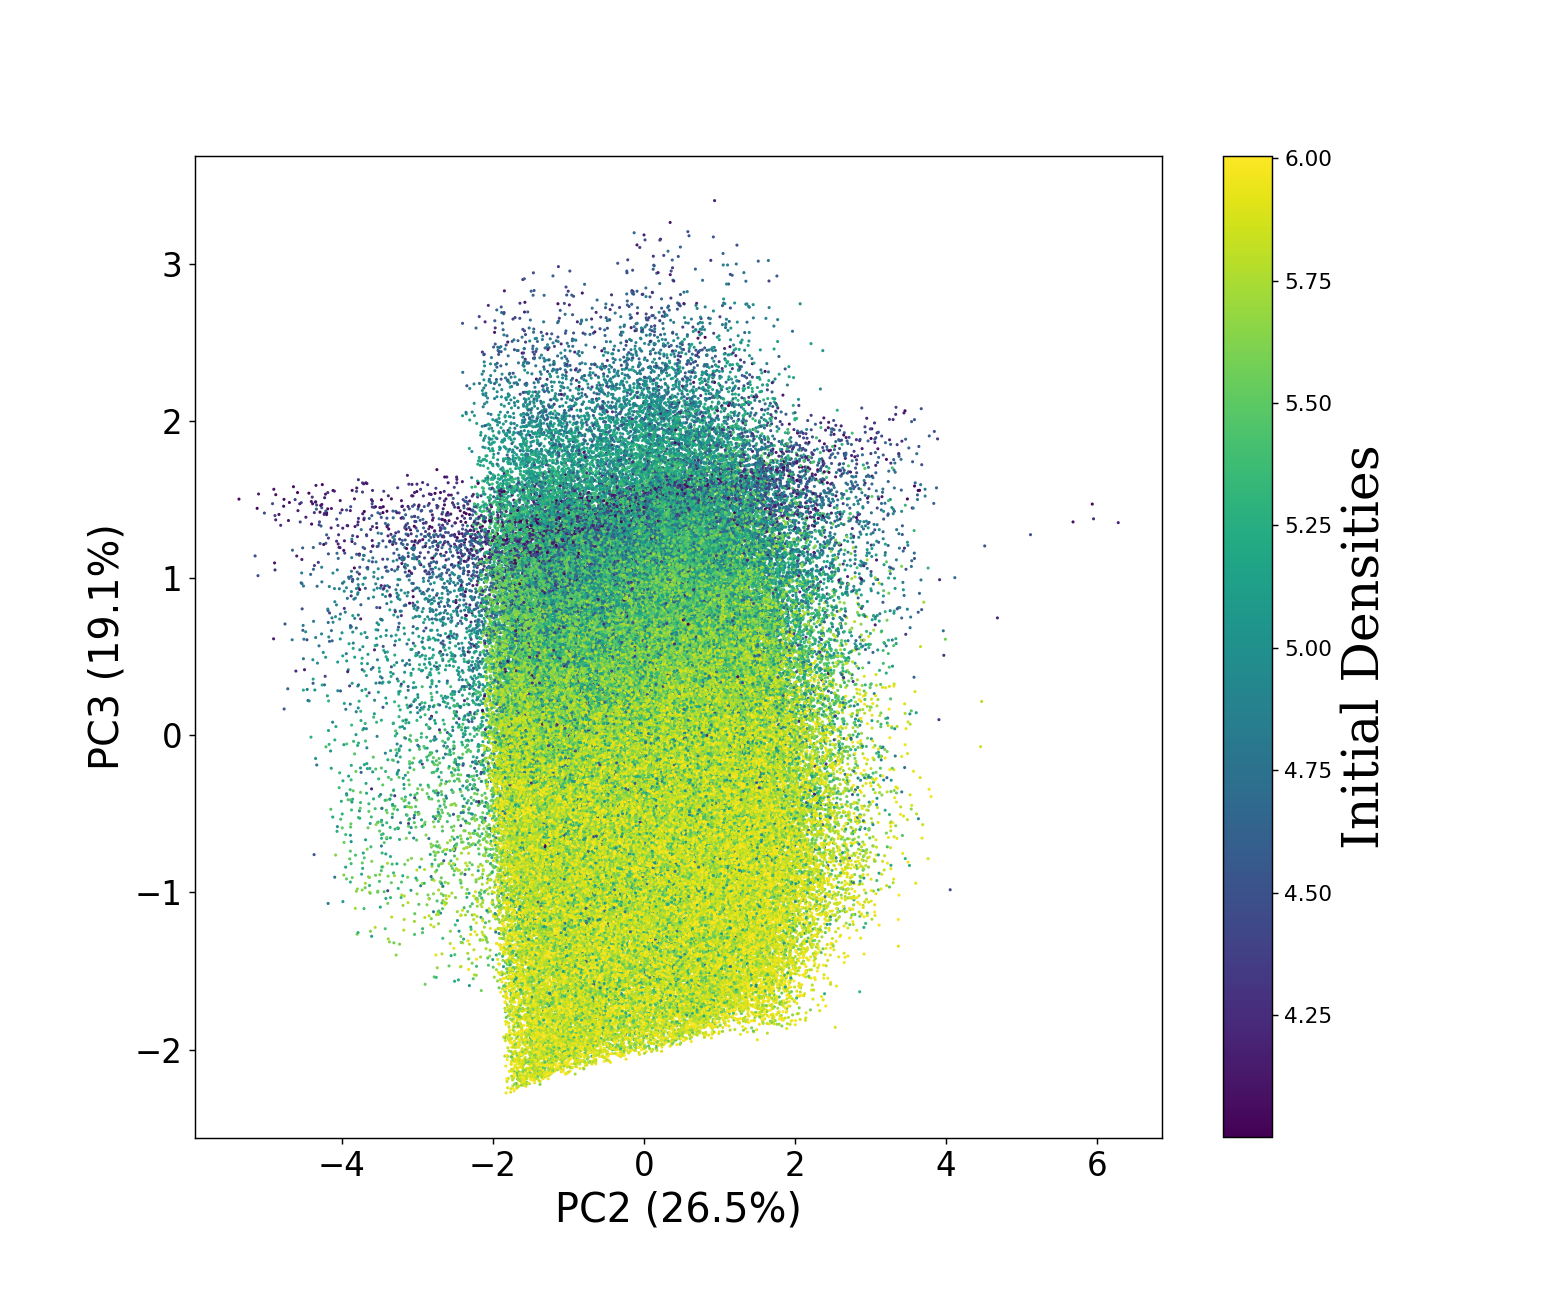
\includegraphics[width=5.9cm]{5/PC2&3_initialDens.png}
}
\caption{Projection of Group C3 (CO, HCO$^+$, CS, SiO, and HCN) on the plane of PC2 and PC3. The top row: max temperature and metallicity. The bottom row: A\textsubscript{V} and initial densities.}
\label{C3-23}
\end{figure*}

 %%%%------------------------------------------
\begin{figure*}[htbp]
\centering
\subfigure{
\label{C3-34-av}
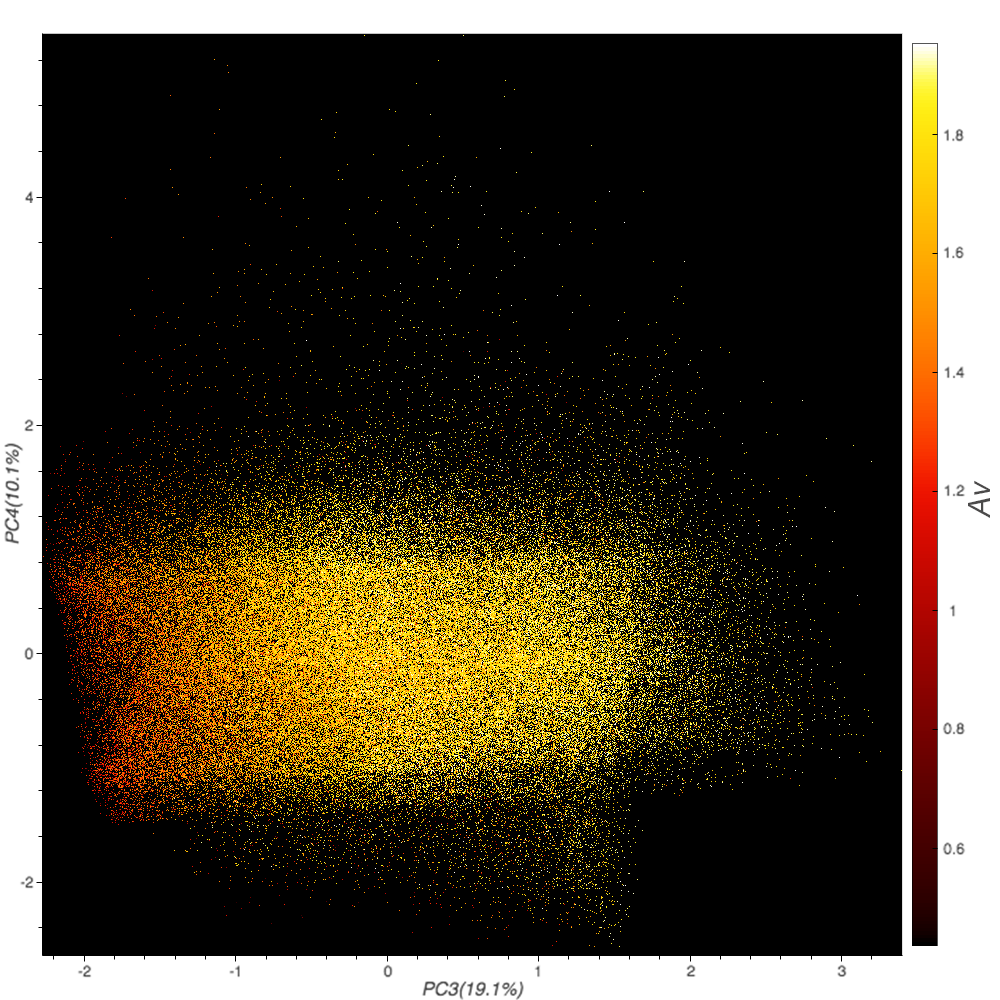
\includegraphics[width=5.9cm]{5/PC3&4_av.png}
}
\subfigure{
\label{C3-34-initialdens}
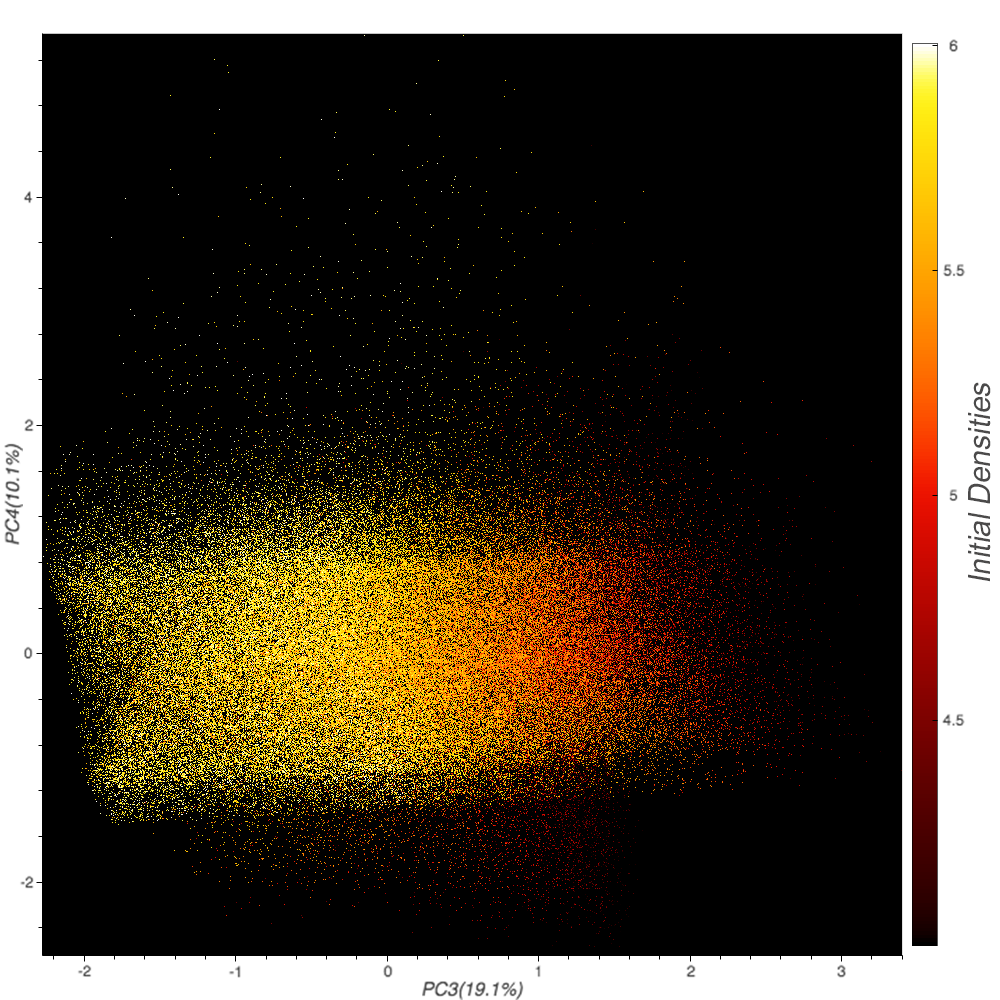
\includegraphics[width=5.9cm]{5/PC3&4_initialDens.png}
}
\caption{Projection of Group C3 (CO, HCO$^+$, CS, SiO, and HCN) on the plane of PC3 and PC4. The first panel is the A\textsubscript{V} and the second panel is the initial densities.}
\label{C3-34}
\end{figure*}

 %%%%%---------------Table 9------------------------------

  \begin{table*}[htbp]
  \centering
  \begin{tabular}{ccccc}
  \hline\hline
  \multirow{2}{*}{Principal Components} & \multicolumn{4}{c}{Physical Parameters}  \\ \cline{2-5} 
                                      & \begin{tabular}[c]{@{}c@{}}maximum \\ temperture\end{tabular} & \multicolumn{1}{l}{metallicity} & \multicolumn{1}{l}{A\textsubscript{V}} & \begin{tabular}[c]{@{}c@{}}initial\\ densities\end{tabular} \\ \hline
PC1 &  & -  & &  \\ \hline
PC2 & - & & &  \\ \hline
PC3 &   &   & +   & -   \\ \hline\hline
  \end{tabular}
  \caption{Changing trend of physical parameters on top three PCs among Group C3 (CO, HCO$^+$, CS, SiO, and HCN)}
  \label{table-5-all}
  \end{table*}
  
  
\subsection{Shock models}

     In this section, the simulation outputs of C-shock model are analyzed by PCA and the corresponding results will be illustrated. 
     A shock-tracer molecular collection: SiO, HCO$^+$, CH$_3$OH, H$_2$CS, HNCO, NH$_3$, OCS, and CO, named as Group S1, is adopted. 
     Besides, the Group S2: CO, HCO$^+$, CS, SiO, HCN, NH$_3$, and HNC, used in Cloud model, is introduced for comparability with previous results. 
     Finally, a combination of the above-mentioned molecules named Group S3 (CO, HCO$^+$, CS, SiO, HCN, HNC, HNCO, CH$_3$OH, and N$_2$H$^+$) is analysed and the results are interpreted in following.
 
 
\subsubsection{Group S1 (SiO, HCO$^+$, CH$_3$OH, H$_2$CS, HNCO, NH$_3$, OCS, and CO)}

    In this section, a group of recognized shock tracers is merged for further analysis. 
    In the outflow of a newborn protostar, shocks heat the gas and trigger a series of reactions such as grain mantle sublimation and sputtering. 
    Molecules such as H$_2$O, NH$_3$, and CH$_3$OH undergo a distinct enhancement of abundance \citep{van1998chemical} and observed at mm-wavelengths \citep{bachiller1997shock,garay1998molecular,jorgensen2007prosac}. 
    Due to the difficulties of being observed on the ground, highly abundant as it is, H$_2$O is less useful as a tracer compared with NH$_3$. 
    CO, SiO, and HNCO are commonly acknowledged shock tracers \citep{martin1997sio,rodriguez2010hnco}, where HNCO is believed to form mainly on the dust grain mantles \citep{lopez2015shedding} or during the gas phase, also viewed as a particularly good tracer of low velocity shocks \citep{kelly2017molecular}. H$_2$CS and OCS are important sulphur carrying molecules in grain mantles \citep{codella2005chemical}. 

    As shown in Fig. \ref{Fig-shock-1-varianve} and Table \ref{table-shock-1-1}, the top three PCs account for more than $80\%$ of total variance (PC1: $49.5\%$, PC2: $18.1\%$, and PC3: $14.9\%$). 
    Loading plots graphically show the influence of molecules having on each of PCs. 
    In the plane of PC1 and PC2, Fig.\ref{Fig-shock-1-loading-12} demonstrates that HCO$^+$ and H$_2$CS are highly correlated, the influence of NH$_3$ having on this plane is trivial. 
    However, Table \ref{table-shock-1-1} shows that NH$_3$ is the most contributive on PC3, owning the eigenvalue of -0.808. 
    Plots of projection on PC1 and PC2 indicate that the density and A\textsubscript{V} are decreasing on the direction of PC1, as shown in Fig. \ref{S1-12-density} and Fig. \ref{S1-12-av}. 
    Fig. \ref{S1-12-velocity} and Fig. \ref{S1-12-temp} reveal that on the PC2, there is a descending trend for velocity and temperature. 
    Table \ref{table-shock-1-3} shows the results in a symbolic way.

%%%%%%------------   Figure ------------------------ 
  \begin{figure}[htbp]
   \centering
   \captionsetup{justification=centering}
   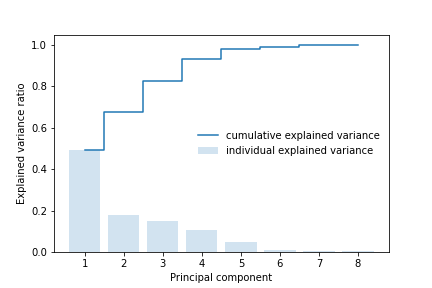
\includegraphics[angle=0,scale =0.6]{shock-1/explained_variance_ratio.png}
   \caption{Individual and cumulative explained variance of PCs among Group S1 (SiO, HCO$^+$, CH$_3$OH, H$_2$CS, HNCO, NH$_3$, OCS, and CO)}
         \label{Fig-shock-1-varianve}
   \end{figure}

\begin{table*}[htbp]
\centering
\begin{tabular}{ccc}
\hline\hline
\multicolumn{1}{l}{Principal Components} & \multicolumn{1}{l}{Explained Ratio} & Cumulative Variance \\ \hline
        PC1 & 0.495  & 0.495\\ 
        PC2 & 0.181  & 0.676\\
        PC3 & 0.149  & 0.825\\
        PC4 & 0.109  & 0.934\\ 
        PC5 & 0.046  & 0.980\\
        PC6 & 0.011  & 0.991\\
        PC7 & 0.006  & 0.997\\
        PC8 & 0.003  & 1.000\\\hline\hline
\end{tabular}
\caption{Table of individual and cumulative explained variance of PCs among Group S1 (SiO, HCO$^+$, CH$_3$OH, H$_2$CS, HNCO, NH$_3$, OCS, and CO)}
\label{table-shock-1-1}
\end{table*}


   
 %%%%%-------------Figure--------
\begin{figure}[htbp]
\centering  
\subfigure[Plane of PC1 and PC2]{
\label{Fig-shock-1-loading-12}
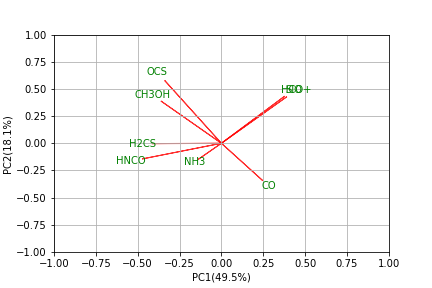
\includegraphics[width=0.5\textwidth]{shock-1/loadingplot_PC1&2.png}}
\subfigure[Plane of PC2 and PC3]{
\label{Fig-shock-1-loading-23}
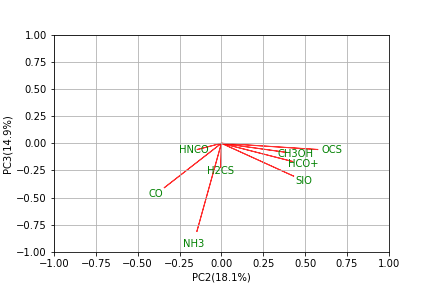
\includegraphics[width=0.5\textwidth]{shock-1/loadingplot_PC2&3.png}}
\caption{Loading plots of Group S1 (SiO, HCO$^+$, CH$_3$OH, H$_2$CS, HNCO, NH$_3$, OCS, and CO)}
\label{Fig-shock-1-loading}
\end{figure}



%%%%%%%%%%---------------Table 5 -----------------
\begin{table*}[htbp]
\centering
\begin{tabular}{ccccccccc}
\hline\hline
\multirow{2}{*}{Molecular Species} & \multicolumn{6}{c}{Principal Components}                 \\ \cline{2-9} 
                                   & 1       & 2       & 3       & 4       & 5      & 6      &7   &8 \\ \hline
SIO   & 0.375  & 0.43   & -0.301 & 0.105  & 0.362  & 0.053  & 0.05   & -0.661  \\ \hline
HCO$^+$   & 0.388  & 0.425  & -0.167 & 0.302  & -0.092 & -0.486 & -0.199 & 0.516  \\ \hline
CH$_3$OH & -0.358 & 0.385  & -0.083 & -0.518 & -0.201 & -0.131 & -0.603 & -0.163 \\ \hline
H$_2$CS  & -0.411 & -0.003 & -0.222 & 0.381  & 0.593  & 0.285  & -0.38  & 0.245 \\ \hline
HNCO  & -0.469 & -0.143 & -0.057 & 0.193  & 0.145  & -0.761 & 0.219  & -0.268 \\ \hline
NH$_3$   & -0.137 & -0.146 & -0.808 & 0.157  & -0.496 & 0.158  & 0.103  & -0.031 \\ \hline
OCS   & -0.336 & 0.574  & -0.057 & -0.225 & 0.104  & 0.144  & 0.624  & 0.288  \\ \hline
CO    & 0.244  & -0.34  & -0.407 & -0.61  & 0.437  & -0.196 & 0.051  & 0.234 \\ \hline\hline
\end{tabular}
\caption{Eigenvalues of PCA among Group S1 (SiO, HCO$^+$, CH$_3$OH, H$_2$CS, HNCO, NH$_3$, OCS, and CO)}
\label{table-shock-1-eigen}
\end{table*}


 %%%%-------------------------------------------
\begin{figure*}[htbp]
\centering
\subfigure{
\label{S1-12-density}
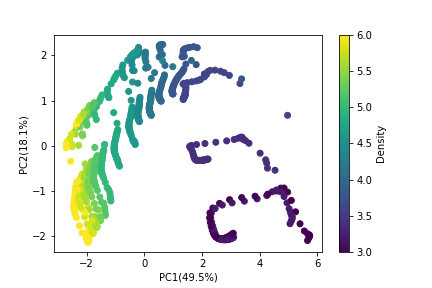
\includegraphics[scale=0.5]{shock-1/PC1&2_Density.png}
} 
\subfigure{
\label{S1-12-av}
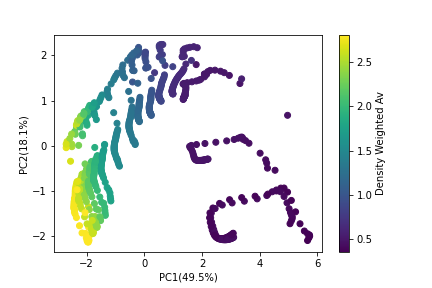
\includegraphics[scale=0.5]{shock-1/PC1&2_av.png}
}
\\
\subfigure{
\label{S1-12-velocity}
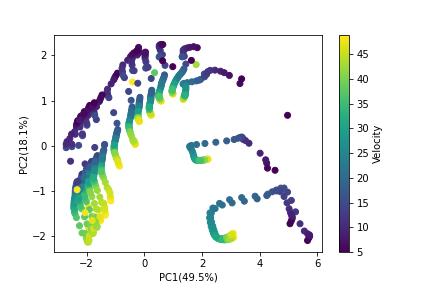
\includegraphics[scale=0.5]{shock-1/PC1&2_Velocity.png}
}
\subfigure{
\label{S1-12-temp}
\includegraphics[scale=0.5]{shock-1/PC1&2_temp.png}
}
\caption{Projection of Group S1 (SiO, HCO$^+$, CH$_3$OH, H$_2$CS, HNCO, NH$_3$, OCS, and CO) on the plane of PC1 and PC2. Two panels on the top row: density and A\textsubscript{V}, two panels on the bottom row: velocity and temperature.}
\label{S1-12}
\end{figure*}

   
   
   
   
   %%%%%---------------Table ------------------------------

  \begin{table*}[htbp]
  \centering
  \begin{tabular}{ccccc}
  \hline\hline
 \multirow{2}{*}{Principal Components} & \multicolumn{4}{c}{Physical Parameters}  \\ \cline{2-5} 
                                      & \begin{tabular}[c]{@{}c@{}}density\end{tabular} & \multicolumn{1}{l}{velocity} & \multicolumn{1}{l}{A\textsubscript{V}} & \begin{tabular}[c]{@{}c@{}}temperature\end{tabular} \\ \hline
PC1 & - &   & - &  \\ \hline
PC2 &  & - & & -  \\ \hline\hline
  \end{tabular}
  \caption{Changing trend of physical parameters on top three PCs among Group S1 (SiO, HCO$^+$, CH$_3$OH, H$_2$CS, HNCO, NH$_3$, OCS, and CO)}
  \label{table-shock-1-3}
  \end{table*}




\subsubsection{Group S2 (CO, HCO$^+$, CS, SiO, HCN, NH$_3$, and HNC)}

    In this section, Group S2 contained seven molecules is introduced and corresponding results are presented in detail. 
    This analysis is expected to create a deliberate contrast between Cloud model and C-shock model. 
    Fig.\ref{Fig-shock-2-varianve} and Table \ref{table-shock-2-1} show the explained variance of seven PCs, where the top three PCs occupy over $90\%$ of cumulative explained variance, accounting for PC1: $53.0\%$, PC2: $20.4\%$, and PC3: $18.1\%$ separately. 
 
 %%%%%%------------   Figure ------------------------ 
  \begin{figure}[htp]
   \centering
   \captionsetup{justification=centering}
   \includegraphics[angle=0,scale =0.6]{shock-2/explained_variance_ratio.png}
   \caption{Individual and cumulative explained variance of PCs among Group S2 (CO, HCO$^+$, CS, SiO, HCN, NH$_3$, and HNC)}
\label{Fig-shock-2-varianve}
   \end{figure}
   
%%--------------    Table  ----------------------

\begin{table*}[htp]
\centering
\begin{tabular}{ccc}
\hline\hline
\multicolumn{1}{l}{Principal Components} & \multicolumn{1}{l}{Explained Ratio} & Cumulative Variance \\ \hline
        PC1 & 0.530  & 0.530\\ 
        PC2 & 0.204  & 0.734\\
        PC3 & 0.181  & 0.915\\
        PC4 & 0.047  & 0.962\\ 
        PC5 & 0.017  & 0.979\\
        PC6 & 0.014  & 0.993\\
        PC7 & 0.007  & 1.000\\\hline\hline
\end{tabular}
\caption{Table of individual and cumulative explained variance of PCs among Group S2 (CO, HCO$^+$, CS, SiO, HCN, NH$_3$, and HNC)}
\label{table-shock-2-1}
\end{table*}

    Fig.\ref{Fig-shock-2-loading-12} and Fig.\ref{Fig-shock-2-loading-23} and Table \ref{table-shock-2-eigen} exhibit the eigenvalues of seven molecules on every PCs. 
    On PC1, the contribution of NH$_3$ is almost negligible, with eigenvalue only 0.04, but the most significant on PC3, where the eigenvalue is -0.809. 
    On PC2, however, CO has the biggest eigenvalue of -0.613. The angle between two molecules on the plane of loading plot (as shown in Fig.\ref{Fig-shock-2-loading-12} and Fig.\ref{Fig-shock-2-loading-23}) reveals that HCO$^+$, SiO and CS are positively correlated and can be taken as a proxy with each other. 
    Same as the correlation between HCN and HNC.


 %%%%-----------
 
\begin{figure}[htp]
\centering  
\subfigure[Plane of PC1 and PC2]{
\label{Fig-shock-2-loading-12}
\includegraphics[width=0.5\textwidth]{shock-2/loadingplot_PC1&2.png}}
\subfigure[Plane of PC2 and PC3]{
\label{Fig-shock-2-loading-23}
\includegraphics[width=0.5\textwidth]{shock-2/loadingplot_PC2&3.png}}
\caption{Loading plots of Group S2 (CO, HCO$^+$, CS, SiO, HCN, NH$_3$, and HNC)}
\label{Fig-shock-2-loading}
\end{figure}


%%------------------TABLE-------------------------------
\begin{table*}[htp]
\centering
\begin{tabular}{cccccccc}
\hline\hline
\multirow{2}{*}{Molecular Species} & \multicolumn{7}{c}{Principal Components}                 \\ \cline{2-8} 
                                   & 1       & 2       & 3       & 4       & 5      & 6    & 7\\ \hline
CO   & -0.293  & -0.613 & -0.052 & -0.634 & -0.138 & -0.103 & 0.319 \\ \hline
HCO+ & -0.424 & 0.423  & -0.117 & 0.139   & -0.515 & 0.237   & 0.534  \\ \hline
CS   & -0.468 & 0.226  & -0.153 & -0.007 & 0.783  & -0.173 & 0.248  \\ \hline
SIO  & -0.452  & 0.312   & -0.163 & -0.340 & -0.224 & -0.202 & -0.681 \\ \hline
HCN  & 0.355  & 0.230  & -0.526  & -0.462 & 0.157  & 0.552   & 0.011  \\ \hline
NH3  & 0.041  & -0.26 & -0.809 & 0.382  & -0.124 & -0.331 & -0.007  \\ \hline
HNC  & 0.425  & 0.413  & 0.022  & -0.319 & -0.104 & -0.669 & 0.294  \\ \hline\hline
\end{tabular}
\caption{Eigenvalues of PCA among Group S2 (CO, HCO$^+$, CS, SiO, HCN, NH$_3$, and HNC)}
\label{table-shock-2-eigen}
\end{table*}

    Figures of projection demonstrate that on PC1, the physical parameter density and A\textsubscript{V} both have an increasing trend, as shown in Fig.\ref{S2-12-density} and Fig.\ref{S2-12-av}. 
    On the PC2, however, velocity and temperature show a decreasing trend, as demonstrated in Fig.\ref{S2-12-velocity} and Fig.\ref{S2-12-temp}. 
    A symbolic record is presented in Table \ref{table-shock-2-3}. 

 %%%%-------------------------------------------
\begin{figure*}[htbp]
\centering
\subfigure{
\label{S2-12-density}
\includegraphics[scale=0.5]{shock-2/PC1&2_Density.png}
} 
\subfigure{
\label{S2-12-av}
\includegraphics[scale=0.5]{shock-2/PC1&2_av.png}
}
\\
\subfigure{
\label{S2-12-velocity}
\includegraphics[scale=0.5]{shock-2/PC1&2_Velocity.png}
}
\subfigure{
\label{S2-12-temp}
\includegraphics[scale=0.5]{shock-2/PC1&2_temp.png}
}
\caption{Projection of Group S2 (CO, HCO$^+$, CS, SiO, HCN, NH$_3$, and HNC) on the plane of PC1 and PC2. Two panels on the top row: density and A\textsubscript{V}, two panels on the bottom row: velocity and temperature.}
\label{S2-12}
\end{figure*}


  %%%%%---------------Table 6------------------------------

  \begin{table*}[htbp]
  \centering
  \begin{tabular}{ccccc}
  \hline\hline
 \multirow{2}{*}{Principal Components} & \multicolumn{4}{c}{Physical Parameters}  \\ \cline{2-5} 
                                      & \begin{tabular}[c]{@{}c@{}}density\end{tabular} & \multicolumn{1}{l}{velocity} & \multicolumn{1}{l}{A\textsubscript{V}} & \begin{tabular}[c]{@{}c@{}}temperature\end{tabular} \\ \hline
PC1 & + &   & + &  \\ \hline
PC2 &  & - & & -  \\ \hline\hline
  \end{tabular}
  \caption{Changing trend of physical parameters on top three PCs among Group S2 (CO, HCO$^+$, CS, SiO, HCN, NH$_3$, and HNC)}
  \label{table-shock-2-3}
  \end{table*}



\subsubsection{Group S3 (CO, HCO$^+$, CS, SiO, HCN, HNC, HNCO, CH$_3$OH, and N$_2$H$^+$)}

    In this section, Group S3 (CO, HCO$^+$, CS, SiO, HCN, HNC, HNCO, CH$_3$OH, and N$_2$H$^+$), a combination of all nine molecules in Group S1 and S2, is analysed to obtain a clear trend on selected orientations. 
    Fig.\ref{Fig-shock3-varianve} provides the individual and cumulative explained variance of nine PCs, Table \ref{table-shock-3-1} records it statistically. The first three PCs count for more than $80\%$ of the total variance (PC1: $60.4\%$, PC2: $19.7\%$, and PC3: $8.8\%$). 

 %%%%%%------------   Figure ------------------------ 
  \begin{figure}[htbp]
   \centering
   \captionsetup{justification=centering}
   \includegraphics[angle=0,scale =0.6]{shock-3/explained_variance_ratio.png}
   \caption{Individual and cumulative explained variance of PCs among Group S3 (CO, HCO$^+$, CS, SiO, HCN, HNC, HNCO, CH$_3$OH, and N$_2$H$^+$)}
         \label{Fig-shock3-varianve}
   \end{figure}
   
%%--------------    Table  ----------------------

\begin{table*}[htbp]
\centering
\begin{tabular}{ccc}
\hline\hline
\multicolumn{1}{l}{Principal Components} & \multicolumn{1}{l}{Explained Ratio} & Cumulative Variance \\ \hline
        PC1 & 0.604  & 0.603\\ 
        PC2 & 0.197  & 0.800\\
        PC3 & 0.088  & 0.888\\
        PC4 & 0.060  & 0.948\\ 
        PC5 & 0.019  & 0.967\\
        PC6 & 0.016  & 0.983\\
        PC7 & 0.011  & 0.994\\
        PC8 & 0.003  & 0.997\\
        PC9 & 0.002  & 0.999\\\hline\hline
\end{tabular}
\caption{Table of individual and cumulative explained variance of PCs among Group S3 (CO, HCO$^+$, CS, SiO, HCN, HNC, HNCO, CH$_3$OH, and N$_2$H$^+$)}
\label{table-shock-3-1}
\end{table*}

    Fig. \ref{Fig-shock-3-loading-12}, Fig. \ref{Fig-shock-3-loading-23} and Table \ref{table-shock-3-eigen} record eigenvalues of nine molecules on each of PCs. CO, HCO$^+$, CS, SiO, and N$_2$H$^+$ have positive performance on the PC1. 
    On the plane of PC1 and PC2, Fig. \ref{Fig-shock-3-loading-12} shows that HCN and HNC are positively correlated, same for HCO$^+$, SiO, CS, and N$_2$H$^+$. Similarly, this correlation is also appearing in the Group S2. 
    For PC2 and PC3, CO is the most significant molecule, having eigenvalue of 0.511 and -0.507 respectively. 

%%%%%%%%%%5---------------FIGUre----------
 \begin{figure}[htbp]
\centering  
\subfigure[Plane of PC1 and PC2]{
\label{Fig-shock-3-loading-12}
\includegraphics[width=0.5\textwidth]{shock-3/loadingplot_PC1&2.png}}
\subfigure[Plane of PC2 and PC3]{
\label{Fig-shock-3-loading-23}
\includegraphics[width=0.5\textwidth]{shock-3/loadingplot_PC2&3.png}}
\caption{Loading plots of Group S3 (CO, HCO$^+$, CS, SiO, HCN, HNC, HNCO, CH$_3$OH, and N$_2$H$^+$)}
\label{Fig-shock-3-loading}
\end{figure}



%%------------------TABLE-------------------------------
\begin{table*}[htbp]
\centering
\begin{tabular}{cccccccccc}
\hline\hline
\multirow{2}{*}{Molecular Species} & \multicolumn{9}{c}{Principal Components}                 \\ \cline{2-10} 
                                   & 1       & 2       & 3       & 4       & 5      & 6    & 7       & 8      & 9   \\ \hline
CO    & 0.200  & 0.511  & -0.507 & 0.370  & -0.414 & -0.190 & -0.135 & -0.276 & 0.022  \\ \hline
HCO$^+$     & 0.374  & -0.342 & 0.043  & -0.027  & 0.081   & -0.280 & -0.300    & -0.314 & -0.682  \\ \hline
CS    & 0.389  & -0.153 & -0.015 & 0.268  & 0.141  & 0.757  & 0.071  & -0.371 & 0.123 \\ \hline
SIO   & 0.380  & -0.264 & -0.206  & 0.113  & -0.388 & 0.137   & 0.176  & 0.704  & -0.180 \\ \hline
HCN   & -0.287 & -0.393 & -0.255 & 0.580  & 0.244  & -0.275 & 0.463  & -0.093 & -0.018 \\ \hline
HNC   & -0.329 & -0.385 & 0.220  & -0.034 & -0.760 & 0.082  & 0.019  & -0.325 & 0.045 \\ \hline
HNCO  & -0.389 & -0.109 & -0.063 & 0.404  & 0.079  & 0.222  & -0.737 & 0.256  & -0.054 \\ \hline
CH$_3$OH & -0.248 & -0.190 & -0.751 & -0.517 & 0.069  & 0.213  & -0.015 & -0.097 & -0.095 \\ \hline
N$_2$H$^+$  & 0.343  & -0.419 & -0.122 & -0.079 & 0.038  & -0.338 & -0.310 & -0.025 & 0.686 \\ \hline\hline
\end{tabular}
\caption{Eigenvalues of PCA among Group S3 (CO, HCO$^+$, CS, SiO, HCN, HNC, HNCO, CH$_3$OH, and N$_2$H$^+$)}
\label{table-shock-3-eigen}
\end{table*}


    As the plot of projection shown in Fig.\ref{S3-12-density} and Fig.\ref{S3-12-av}, the physical parameter density and A\textsubscript{V} have a declining trend in the direction of PC1. 
    Conversely, Fig.\ref{S3-12-velocity} and Fig.\ref{S3-12-temp} indicate that velocity and temperature have an increasing trend on PC2. 
    Table \ref{table-shock-3-3} shows these trend symbolically. 

%%%%%%---------------
\begin{figure*}[htbp]
\centering
\subfigure{
\label{S3-12-density}
\includegraphics[scale=0.5]{shock-3/PC1&2_density.png}
} 
\subfigure{
\label{S3-12-av}
\includegraphics[scale=0.5]{shock-3/PC1&2_av.png}
}
\\
\subfigure{
\label{S3-12-velocity}
\includegraphics[scale=0.5]{shock-3/PC1&2_vel.png}
}
\subfigure{
\label{S3-12-temp}
\includegraphics[scale=0.5]{shock-3/PC1&2_temp.png}
}
\caption{Projection of Group S3 (CO, HCO$^+$, CS, SiO, HCN, HNC, HNCO, CH$_3$OH, and N$_2$H$^+$) on the plane of PC1 and PC2. Two panels on the top row: density and A\textsubscript{V}, two panels on the bottom row: velocity and temperature.}
\label{S3-12}
\end{figure*}

  %%%%%---------------Table-----------------------------

  \begin{table*}[htp]
  \centering
  \begin{tabular}{ccccc}
  \hline\hline
 \multirow{2}{*}{Principal Components} & \multicolumn{4}{c}{Physical Parameters}  \\ \cline{2-5} 
                                      & \begin{tabular}[c]{@{}c@{}}density\end{tabular} & \multicolumn{1}{l}{velocity} & \multicolumn{1}{l}{A\textsubscript{V}} & \begin{tabular}[c]{@{}c@{}}temperature\end{tabular} \\ \hline
PC1 & - &   & - &  \\ \hline
PC2 &  & + & & +  \\ \hline\hline
  \end{tabular}
  \caption{Changing trend of physical parameters on top three PCs among Group S3 (CO, HCO$^+$, CS, SiO, HCN, HNC, HNCO, CH$_3$OH, and N$_2$H$^+$)}
  \label{table-shock-3-3}
  \end{table*}




\section{Conclusions}

   \begin{enumerate}
      \item 
      PC1, PC2, and PC3 are the most significant principal components among both Cloud and C-shock models generated by UCLCHEM simulation after PCA has been applied. 
      For Cloud models, they represent $85.2\%$, $87.4\%$, and $88.3\%$ in the group of 7 molecules, 6 molecules, and 5 molecules respectively.
      As for C-shock models, the cumulative variance is $82.5\%$, $88.8\%$, and $91.5\%$ for group of 8 molecules, 7 molecules, and 9 molecules separately. 
      
      \item 
      For the Cloud models, the molecule CO and NH3, HNC, and HCN are positively correlated on the plane of PC1 and PC2, while the contribution of SiO is almost negligible on this plane. 
      On PC3, the SiO contains overwhelming information, possessing the eigenvalue of 0.944, 0.979, and 0.972 for the group of 7 molecules, 6 molecules, and 5 molecules severally.
      For Cloud models, HNC and HNC have positive correlation with each other.
      Similarly, HCO$^+$, SiO and CS are positively correlated, so they can be viewed as a proxy with each other. 
      This correlation also happens for all C-shock models.
      
      \item 
      For Cloud models, the trend on PCs showing on the projection, as shown in Table \ref{table-7-all}, Table \ref{table-6-all} and Table \ref{table-5-all}, the metallicity and initial densities has a decreasing trend along the direction of PC1 and PC3 respectively, while the A\textsubscript{V} increases on PC3.
      These trends are identical among three different sets of molecules. 
      For C-shock model, Table \ref{table-shock-1-3}, Table \ref{table-shock-2-3} and Table \ref{table-shock-3-3} demonstrate that density and A\textsubscript{V} share the same trend, however, velocity and temperature have consistent changes. 
      
      \item 
      For Cloud models, the physical parameter maximum temperature is too special to be ignored.
      In the group of 7 molecules and 6 molecules, the maximum temperature shows an increasing trend on PC2, where HCO$^+$, the most influential molecule, possesses the eigenvalue of 0.728 and 0.725 separately. 
      However, the maximum temperature has a decreasing trend in the group of 5 molecules, where the eigenvalue of HCO$^+$ is -0.772. 
      It can be concluded that the molecule HCO$^+$, the physical parameter maximum temperature, and the PC2, are highly correlated. 
      When the eigenvalue of HCO$^+$ on PC2 is positive, the maximum temperature shows an increasing trend. 
      While the HCO$^+$ has a negative eigenvalue on PC2, the maximum temperature will have a decreasing tendency on this PC. 
      
      
      \item 
      For C-shock models, the projection of three different molecular groups indicate that the mixed combination, signed as Group S3 (CO, HCO$^+$, CS, SiO, HCN, HNC, HNCO, CH$_3$OH, and N$_2$H$^+$), shows a more obvious trend on the selected PCs, compared with that of shock tracers and seven molecules used in Cloud model. 
      It can postulate that this molecular combination contains a constructive purpose for the further research and observation associated.
      
      \item 
      For C-shock models, HCO$^+$, SiO, and CS are positively correlated, which could be seen in both Gourp S2 and Gourp S3. 
      In Group S2 and S3, the molecule CO is quite important in PC2. 
      When the Group contains NH$_3$, this molecule is the most vital one in PC3. 
      For both Cloud and C-shock models, HCN and HNC are consistently positively-associated. 
      
      
   \end{enumerate}
   
  


% WARNING
%-------------------------------------------------------------------
% Please note that we have included the references to the file aa.dem in
% order to compile it, but we ask you to:
%
% - use BibTeX with the regular commands:
%   \bibliographystyle{aa} % style aa.bst
%   \bibliography{Yourfile} % your references Yourfile.bib
%
% - join the .bib files when you upload your source files
%-------------------------------------------------------------------
\bibliographystyle{aa}
%\thebibliography{plainnat}
\bibliography{reference}


\end{CJK*}
\end{document}
